\documentclass[12pt]{extarticle}
\usepackage[paperwidth=15in,paperheight=8.5in]{geometry}
\usepackage{amsmath}
\usepackage{hyperref}
\usepackage{multirow}
\usepackage{pdfpages}
\usepackage[utf8]{inputenc}
\title{Kaon mixing: chiral and continuum extrapolations}
\author{R Mukherjee}
\date{\today}
\begin{document}
\maketitle
\tableofcontents
\clearpage
\begin{figure}
\centering
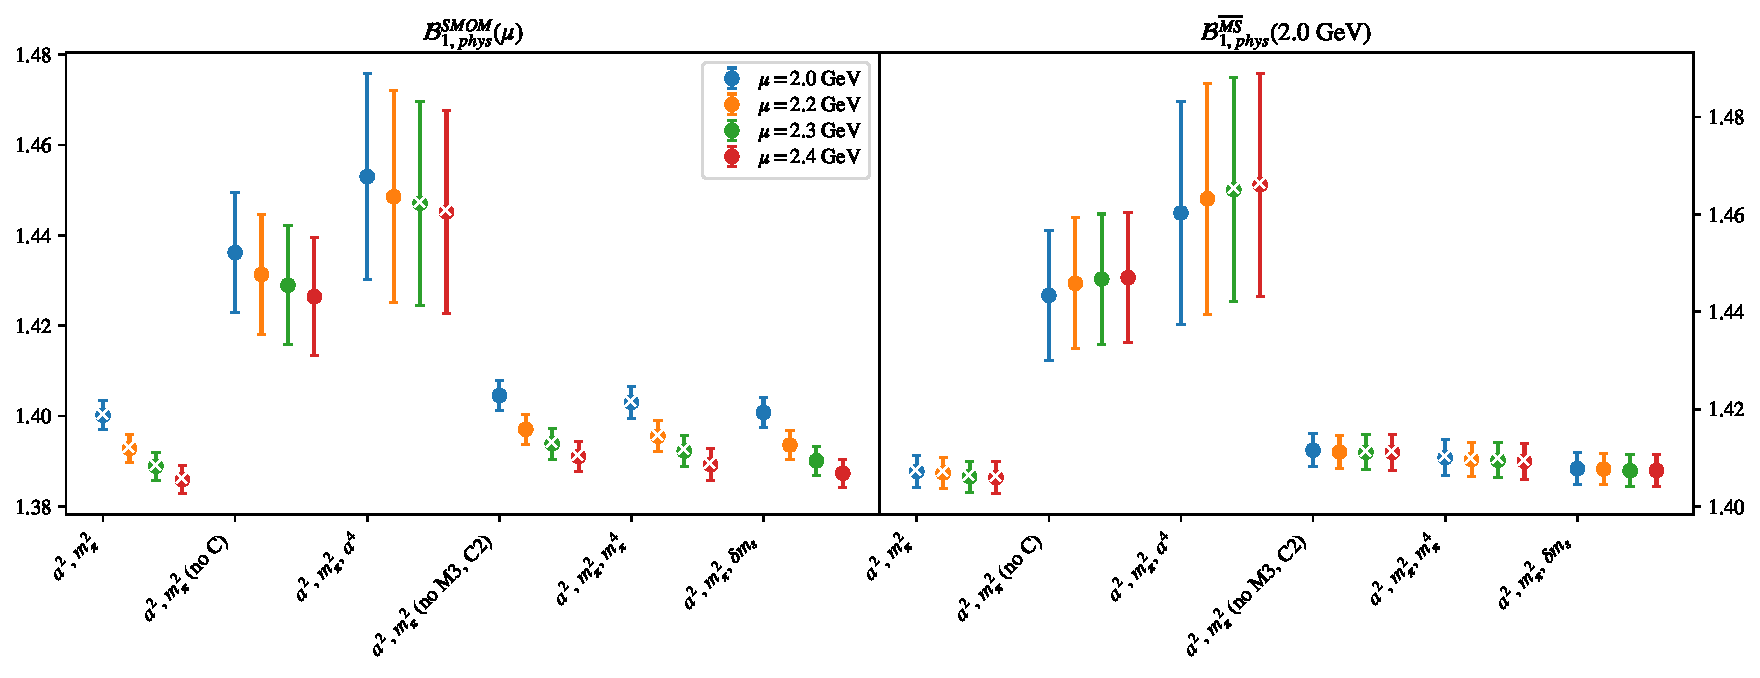
\includegraphics[page=1, width=1.1\textwidth]{VVpAA/NPR/fit_summary_bag.pdf}
\caption{$\mathcal{B}_{1}$\\(left) $\mathcal{B}_{phys}$ in RI/SMOM scheme from fit variations (fits with $p$-value $<0.05$ marked with ``$\times$"). \\(right) $\mathcal{B}_{phys}$ in $\overline{MS}$ computed using $\mathcal{B}^{\overline{MS}} = R^{\overline{MS}\leftarrow SMOM}(2.0)\sigma_{npt}(2.0,\mu) \mathcal{B}^{SMOM}(\mu)$.}
\end{figure}
\clearpage
\begin{figure}
\centering
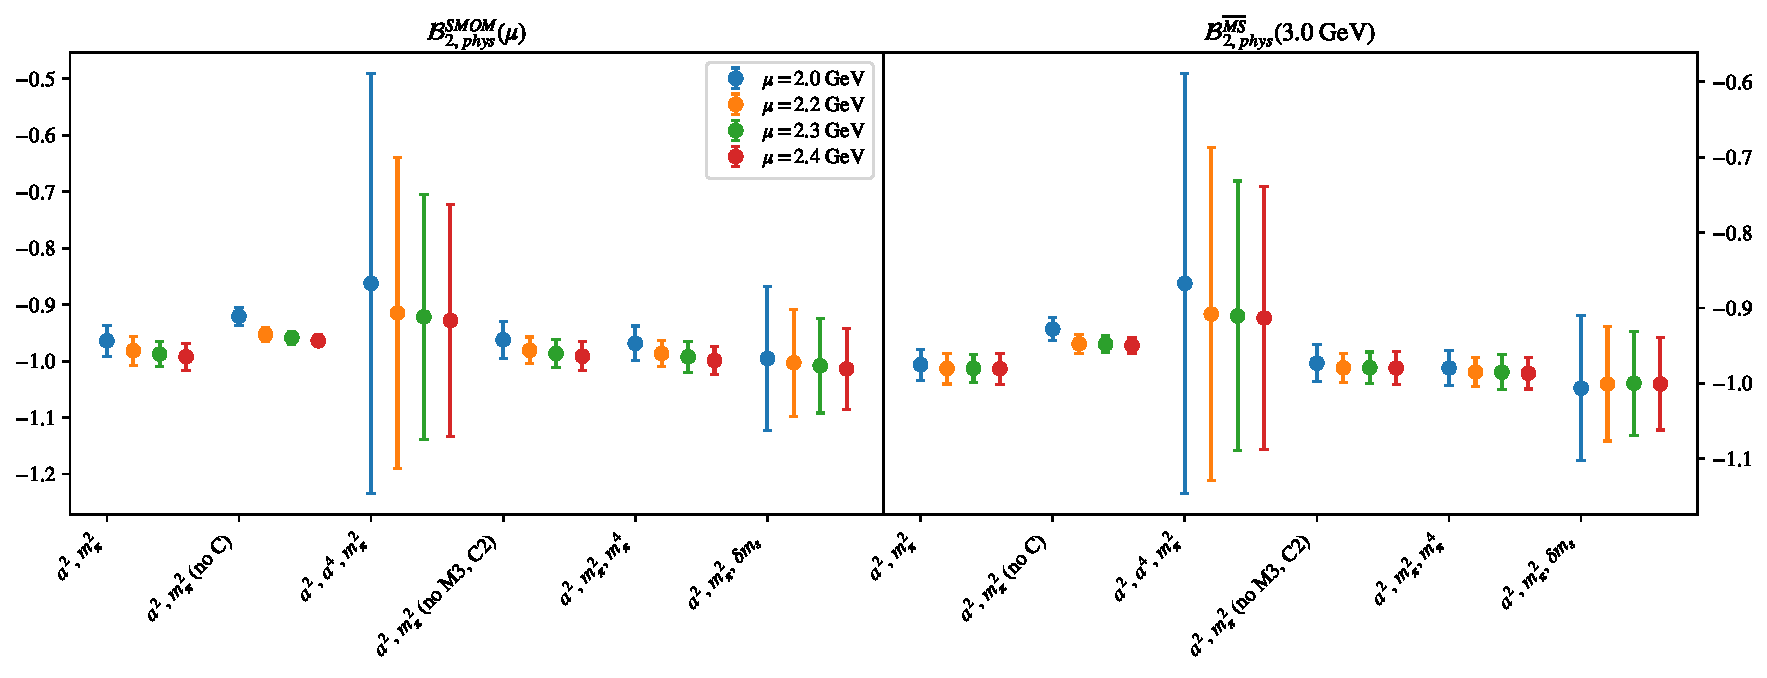
\includegraphics[page=1, width=1.1\textwidth]{VVmAA/NPR/fit_summary_bag.pdf}
\caption{$\mathcal{B}_{2}$\\(left) $\mathcal{B}_{phys}$ in RI/SMOM scheme from fit variations (fits with $p$-value $<0.05$ marked with ``$\times$"). \\(right) $\mathcal{B}_{phys}$ in $\overline{MS}$ computed using $\mathcal{B}^{\overline{MS}} = R^{\overline{MS}\leftarrow SMOM}(3.0)\sigma_{npt}(3.0,\mu) \mathcal{B}^{SMOM}(\mu)$.}
\end{figure}
\clearpage
\begin{figure}
\centering
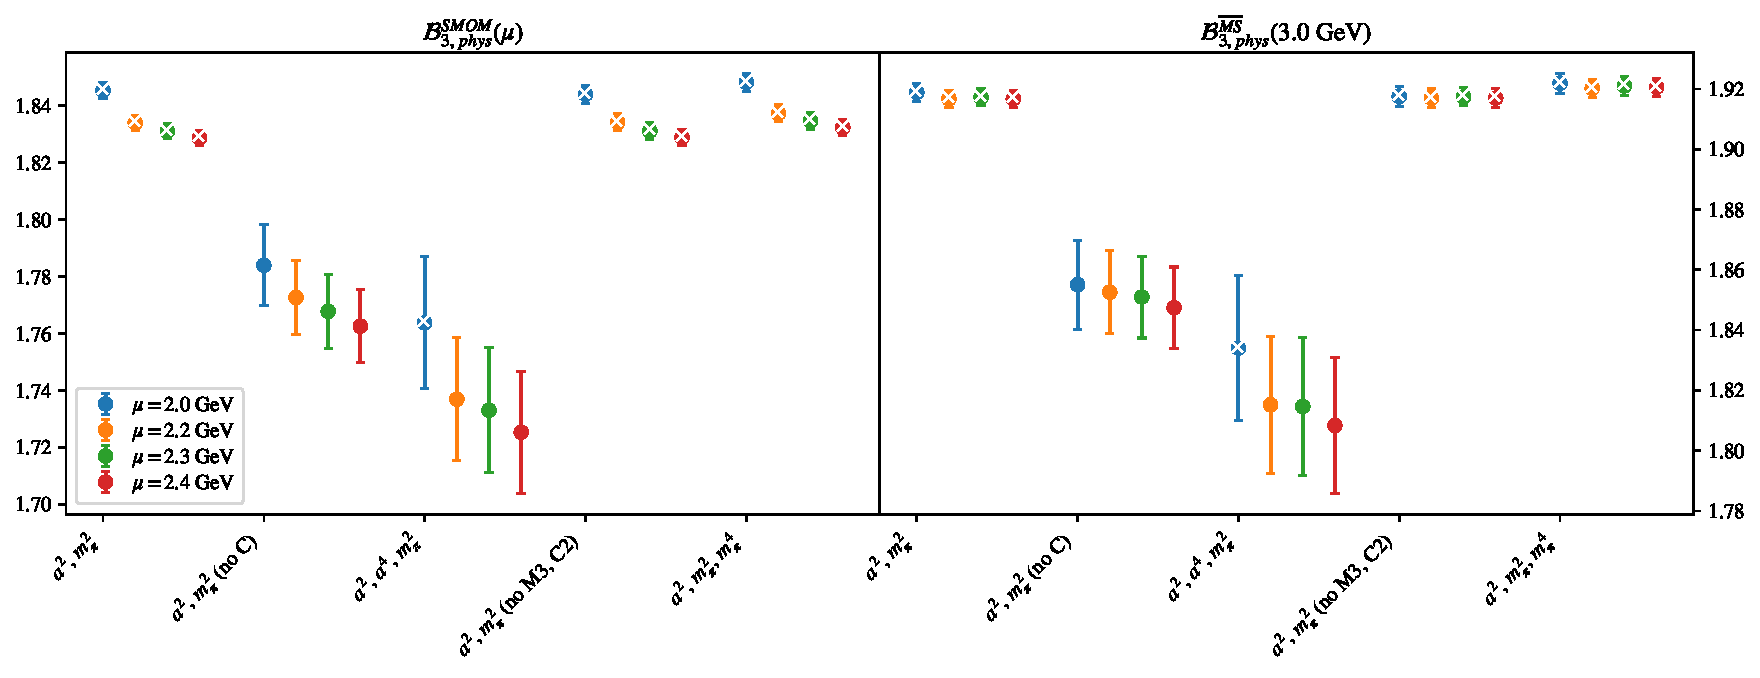
\includegraphics[page=1, width=1.1\textwidth]{SSmPP/NPR/fit_summary_bag.pdf}
\caption{$\mathcal{B}_{3}$\\(left) $\mathcal{B}_{phys}$ in RI/SMOM scheme from fit variations (fits with $p$-value $<0.05$ marked with ``$\times$"). \\(right) $\mathcal{B}_{phys}$ in $\overline{MS}$ computed using $\mathcal{B}^{\overline{MS}} = R^{\overline{MS}\leftarrow SMOM}(3.0)\sigma_{npt}(3.0,\mu) \mathcal{B}^{SMOM}(\mu)$.}
\end{figure}
\clearpage
\begin{figure}
\centering
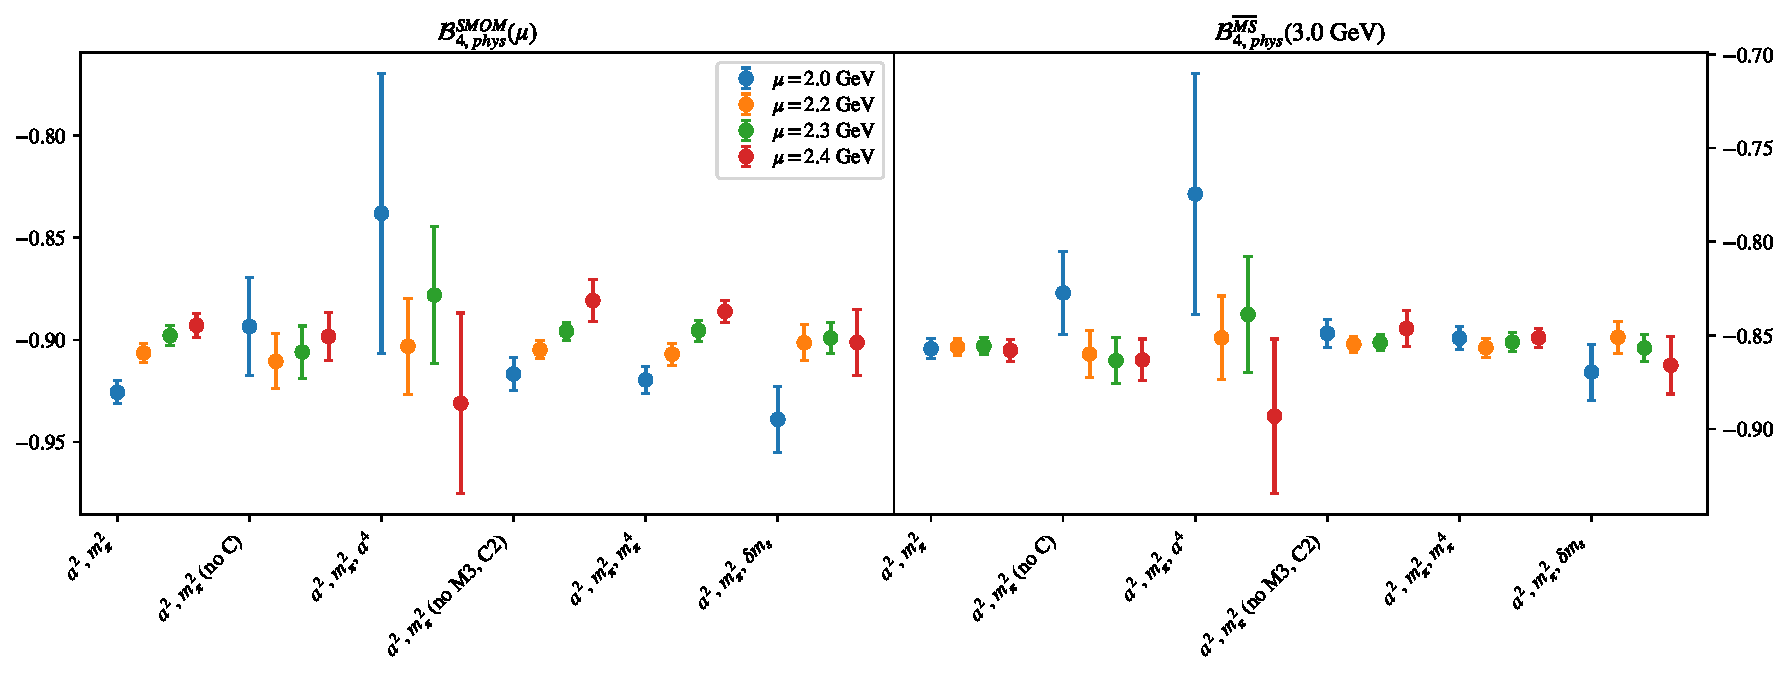
\includegraphics[page=1, width=1.1\textwidth]{SSpPP/NPR/fit_summary_bag.pdf}
\caption{$\mathcal{B}_{4}$\\(left) $\mathcal{B}_{phys}$ in RI/SMOM scheme from fit variations (fits with $p$-value $<0.05$ marked with ``$\times$"). \\(right) $\mathcal{B}_{phys}$ in $\overline{MS}$ computed using $\mathcal{B}^{\overline{MS}} = R^{\overline{MS}\leftarrow SMOM}(3.0)\sigma_{npt}(3.0,\mu) \mathcal{B}^{SMOM}(\mu)$.}
\end{figure}
\clearpage
\begin{figure}
\centering
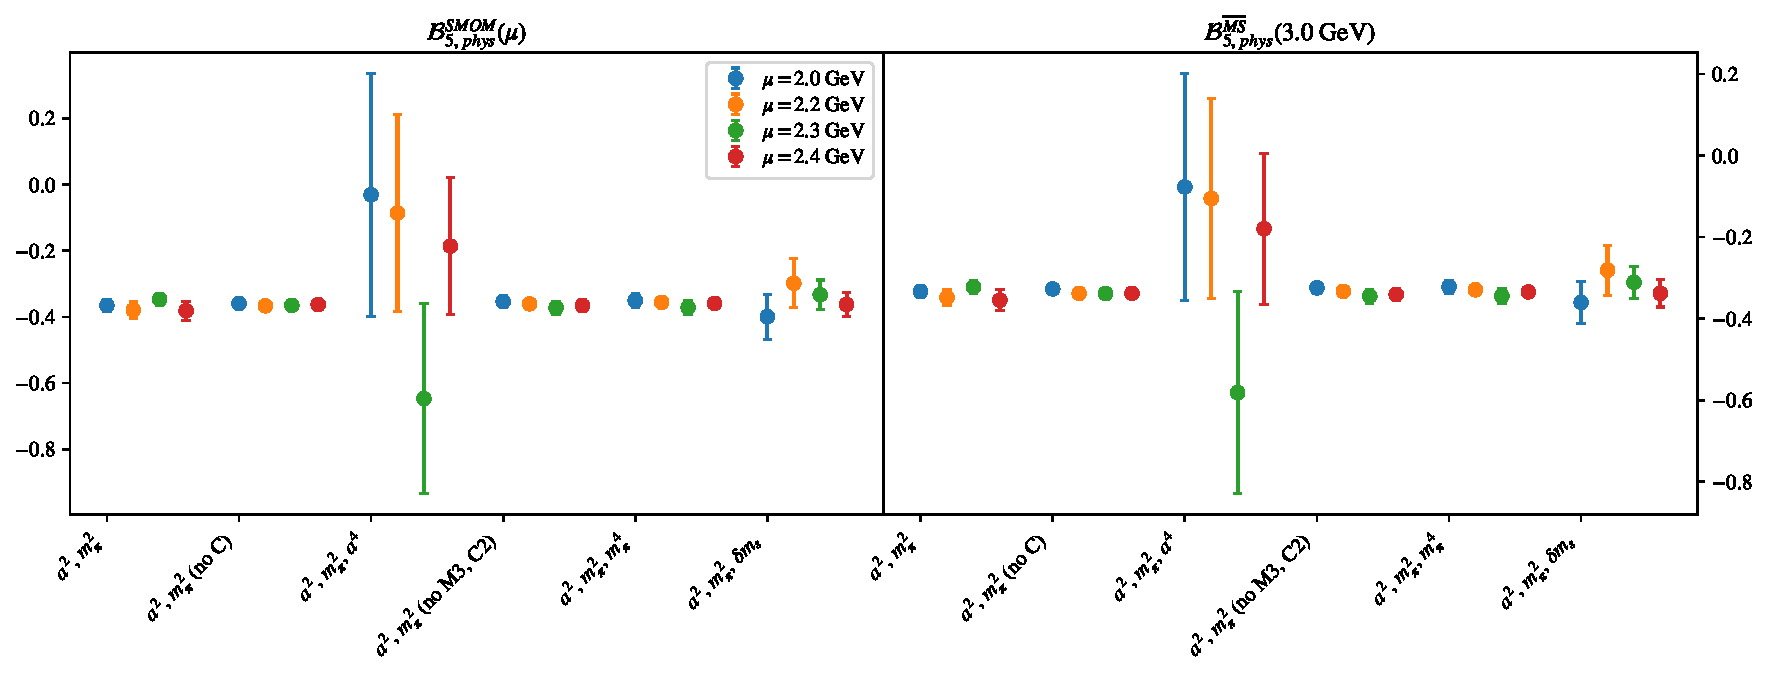
\includegraphics[page=1, width=1.1\textwidth]{TT/NPR/fit_summary_bag.pdf}
\caption{$\mathcal{B}_{5}$\\(left) $\mathcal{B}_{phys}$ in RI/SMOM scheme from fit variations (fits with $p$-value $<0.05$ marked with ``$\times$"). \\(right) $\mathcal{B}_{phys}$ in $\overline{MS}$ computed using $\mathcal{B}^{\overline{MS}} = R^{\overline{MS}\leftarrow SMOM}(3.0)\sigma_{npt}(3.0,\mu) \mathcal{B}^{SMOM}(\mu)$.}
\end{figure}
\clearpage
\section{$\mathcal{B}_1$}
\begin{table}[h!]
\begin{center}
\begin{tabular}{|c|c|c|c|c|c|}
\hline
$\mu$ (GeV) & $a^2$, $m_\pi^2$& $a^2$, $m_\pi^2$ (no C)& $a^2$, $m_\pi^2$, $a^4$& $a^2$, $m_\pi^2$ (no M3, C2)& $a^2$, $m_\pi^2$, $\delta m_s$\\
\hline
2.0& \hyperlink{VVpAA/NPR/bag_a2m2_20.pdf.1}{\textbf{1.4010(30)}: 2.679 (0.02)} & \hyperlink{VVpAA/NPR/bag_a2m2noC_20.pdf.1}{\textbf{1.435(13)}: 0.271 (0.763)} & \hyperlink{VVpAA/NPR/bag_a2a4m2_20.pdf.1}{\textbf{1.451(23)}: 2.068 (0.082)} & \hyperlink{VVpAA/NPR/bag_a2m2mcut_20.pdf.1}{\textbf{1.4051(34)}: 2.153 (0.091)} & \hyperlink{VVpAA/NPR/bag_a2m2delm_20.pdf.1}{\textbf{1.4011(32)}: 1.373 (0.24)}\\
2.2& \hyperlink{VVpAA/NPR/bag_a2m2_22.pdf.1}{\textbf{1.3936(30)}: 3.117 (0.008)} & \hyperlink{VVpAA/NPR/bag_a2m2noC_22.pdf.1}{\textbf{1.431(13)}: 0.3 (0.741)} & \hyperlink{VVpAA/NPR/bag_a2a4m2_22.pdf.1}{\textbf{1.450(23)}: 2.286 (0.058)} & \hyperlink{VVpAA/NPR/bag_a2m2mcut_22.pdf.1}{\textbf{1.3980(33)}: 2.553 (0.054)} & \hyperlink{VVpAA/NPR/bag_a2m2delm_22.pdf.1}{\textbf{1.3939(32)}: 1.389 (0.235)}\\
2.3& \hyperlink{VVpAA/NPR/bag_a2m2_23.pdf.1}{\textbf{1.3900(30)}: 3.511 (0.004)} & \hyperlink{VVpAA/NPR/bag_a2m2noC_23.pdf.1}{\textbf{1.429(13)}: 0.319 (0.727)} & \hyperlink{VVpAA/NPR/bag_a2a4m2_23.pdf.1}{\textbf{1.449(23)}: 2.465 (0.043)} & \hyperlink{VVpAA/NPR/bag_a2m2mcut_23.pdf.1}{\textbf{1.3946(33)}: 2.865 (0.035)} & \hyperlink{VVpAA/NPR/bag_a2m2delm_23.pdf.1}{\textbf{1.3903(32)}: 1.561 (0.182)}\\
2.4& \hyperlink{VVpAA/NPR/bag_a2m2_24.pdf.1}{\textbf{1.3870(30)}: 3.487 (0.004)} & \hyperlink{VVpAA/NPR/bag_a2m2noC_24.pdf.1}{\textbf{1.426(13)}: 0.335 (0.716)} & \hyperlink{VVpAA/NPR/bag_a2a4m2_24.pdf.1}{\textbf{1.446(23)}: 2.546 (0.037)} & \hyperlink{VVpAA/NPR/bag_a2m2mcut_24.pdf.1}{\textbf{1.3917(33)}: 2.887 (0.034)} & \hyperlink{VVpAA/NPR/bag_a2m2delm_24.pdf.1}{\textbf{1.3874(31)}: 1.62 (0.166)}\\
\hline
\end{tabular}
\caption{Physical point value from chiral and continuum extrapolation at renormalisation scale $\mu$. Entries are \textbf{value(error)}: $\chi^2/\text{DOF}$ ($p$-value).}
\end{center}
\end{table}
\begin{table}[h!]
\begin{center}
\begin{tabular}{|c c|c|c|c|c|c|}
\hline
$\mu$ (GeV) &  & $a^2$, $m_\pi^2$& $a^2$, $m_\pi^2$ (no C)& $a^2$, $m_\pi^2$, $a^4$& $a^2$, $m_\pi^2$ (no M3, C2)& $a^2$, $m_\pi^2$, $\delta m_s$\\
\hline
\multirow{3}{0.5in}{2.0} & $\alpha$ & 0.143(11)& -0.048(81)& -0.32(21)& 0.131(12)& 0.147(11)\\
 & $\beta$ & 0.00412(22)& 0.00347(41)& 0.00438(26)& 0.00344(36)& 0.00539(51)\\
 & $\gamma$ &  &  & 0.95(43)&  & -0.049(18)\\
\hline
\multirow{3}{0.5in}{2.2} & $\alpha$ & 0.149(11)& -0.062(81)& -0.38(21)& 0.135(11)& 0.153(11)\\
 & $\beta$ & 0.00399(22)& 0.00334(41)& 0.00429(25)& 0.00328(35)& 0.00539(50)\\
 & $\gamma$ &  &  & 1.07(43)&  & -0.054(18)\\
\hline
\multirow{3}{0.5in}{2.3} & $\alpha$ & 0.152(10)& -0.067(80)& -0.39(21)& 0.137(11)& 0.156(11)\\
 & $\beta$ & 0.00395(22)& 0.00329(41)& 0.00426(25)& 0.00322(35)& 0.00542(49)\\
 & $\gamma$ &  &  & 1.11(43)&  & -0.057(17)\\
\hline
\multirow{3}{0.5in}{2.4} & $\alpha$ & 0.153(10)& -0.068(81)& -0.39(21)& 0.138(12)& 0.156(11)\\
 & $\beta$ & 0.00393(22)& 0.00325(41)& 0.00425(25)& 0.00319(35)& 0.00541(49)\\
 & $\gamma$ &  &  & 1.11(42)&  & -0.057(17)\\
\hline
\end{tabular}
\caption{Fit values of coefficients in $Q = Q_{phys} + \mathbf{\alpha} a^2 + \mathbf{\beta}\left(\frac{m_\pi^2}{f_\pi^2}-\frac{m_{\pi,PDG}^2}{f_\pi^2}\right) + \gamma(\ldots)$}
\end{center}
\end{table}
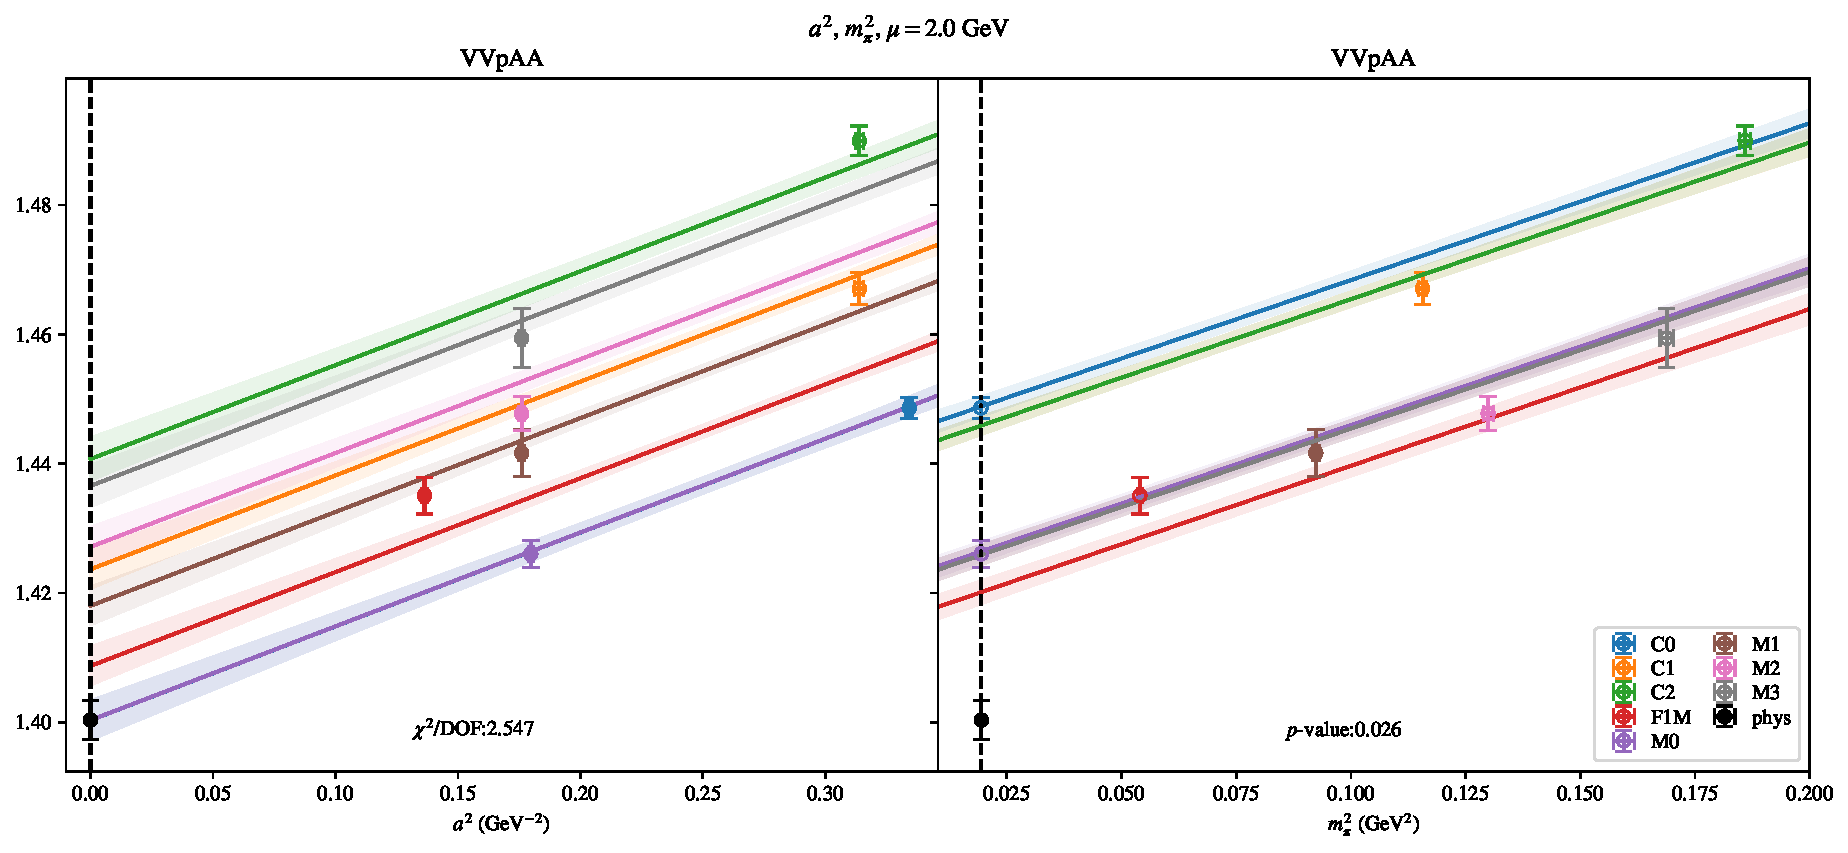
\includepdf[link, pages=-]{VVpAA/NPR/bag_a2m2_20.pdf}
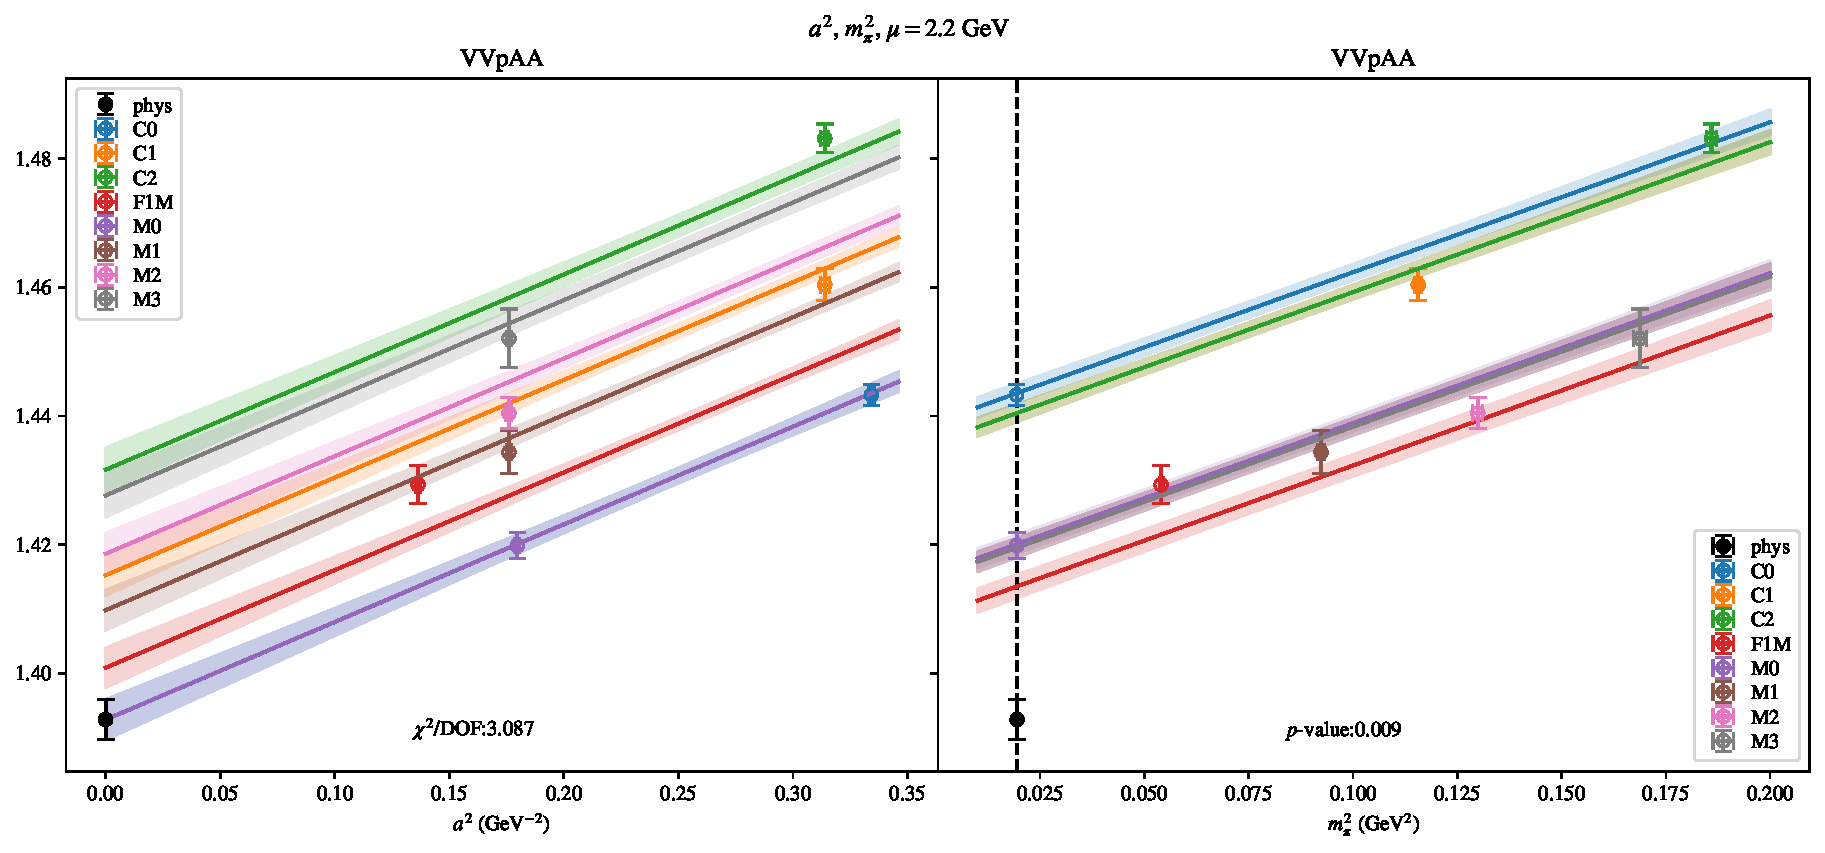
\includepdf[link, pages=-]{VVpAA/NPR/bag_a2m2_22.pdf}
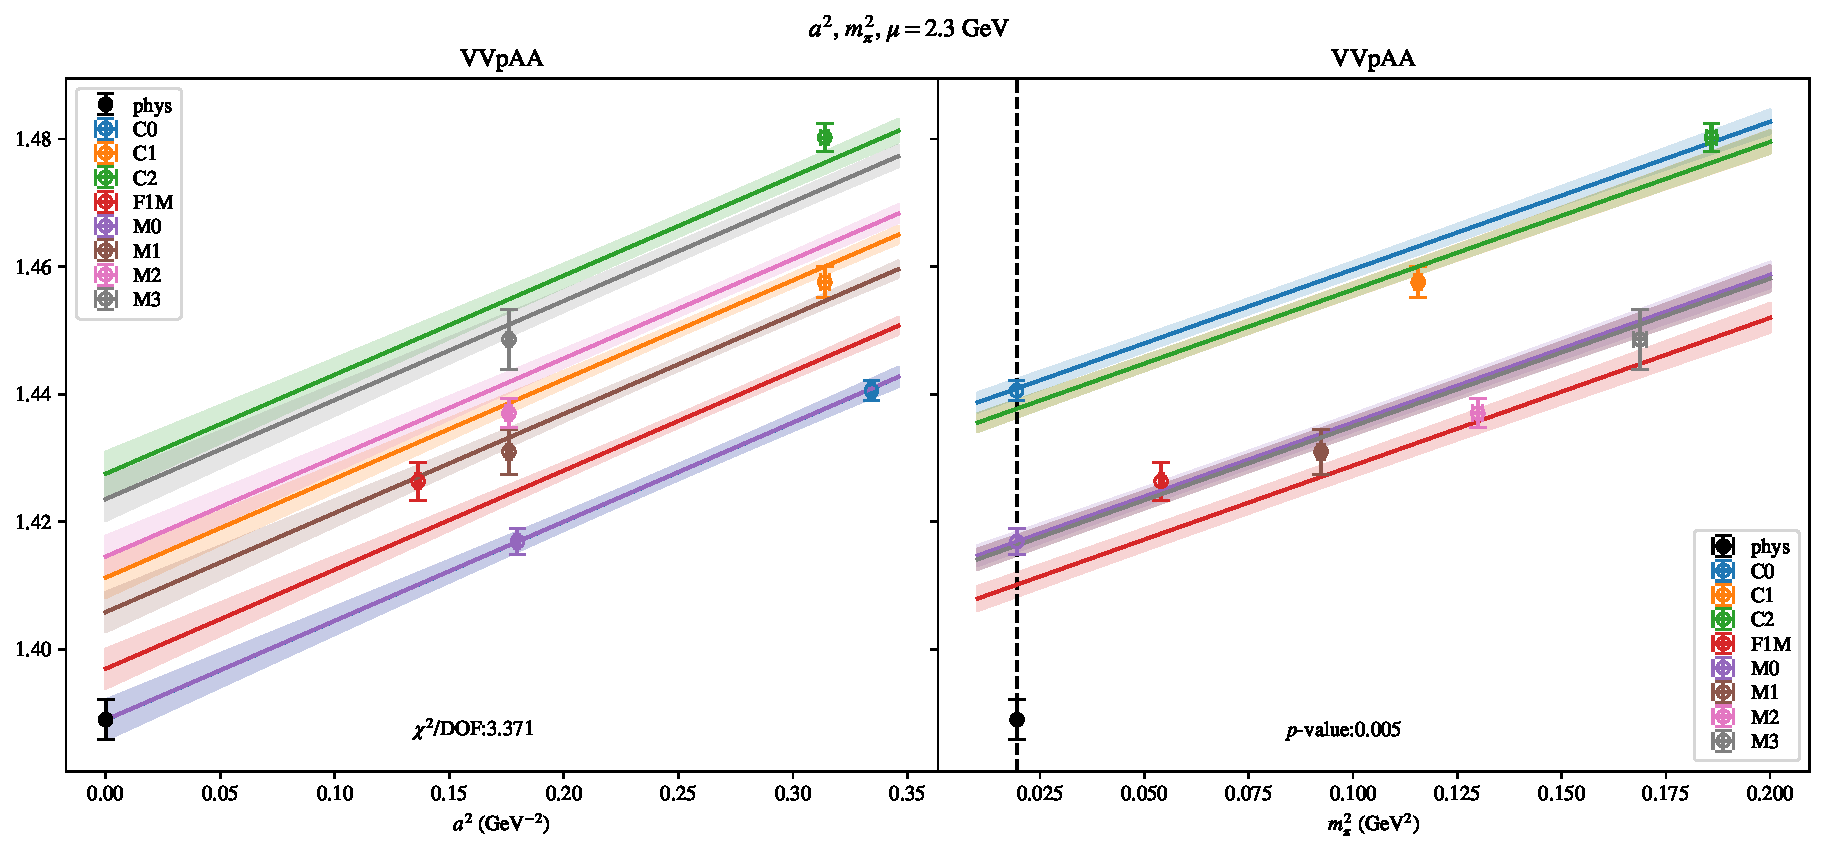
\includepdf[link, pages=-]{VVpAA/NPR/bag_a2m2_23.pdf}
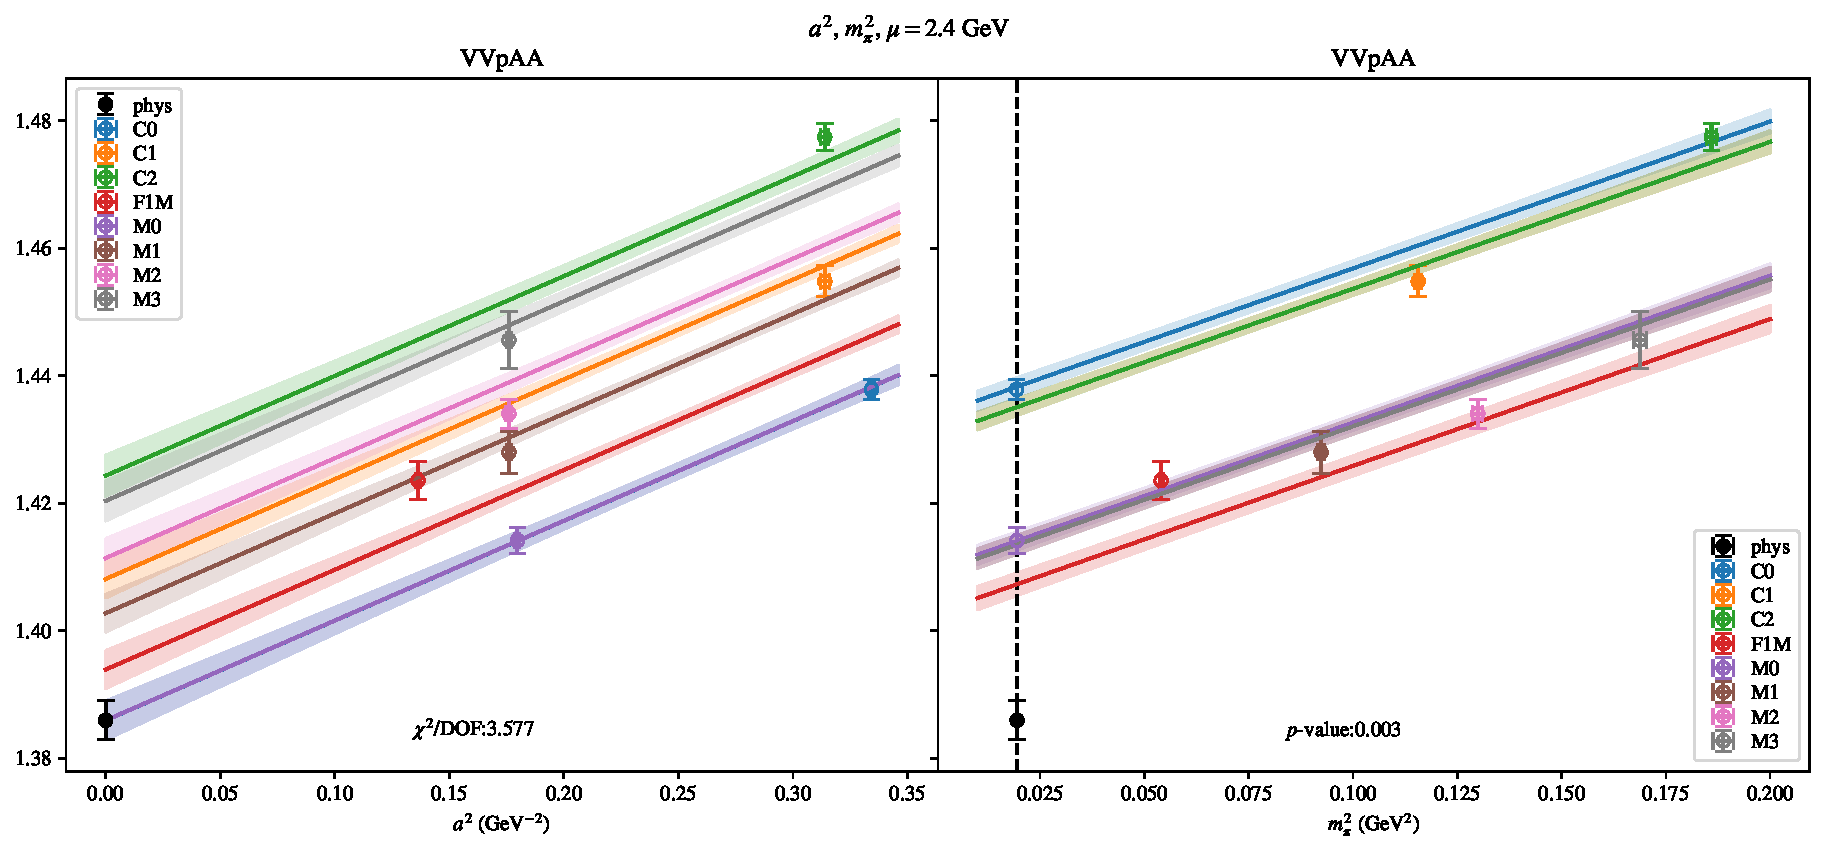
\includepdf[link, pages=-]{VVpAA/NPR/bag_a2m2_24.pdf}
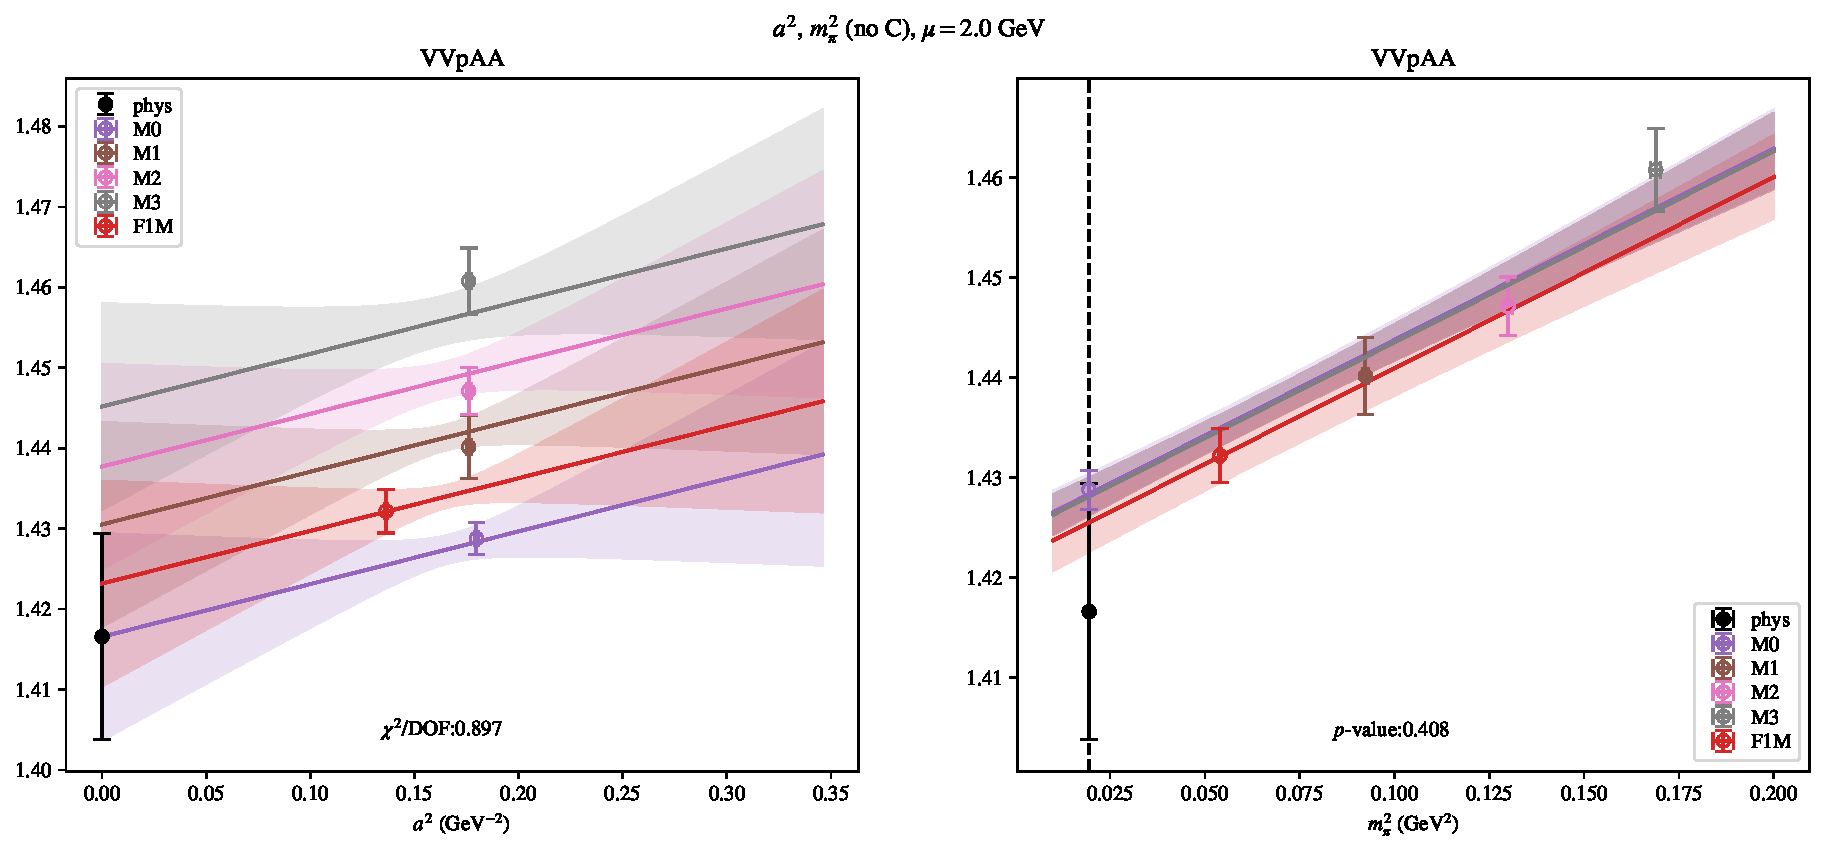
\includepdf[link, pages=-]{VVpAA/NPR/bag_a2m2noC_20.pdf}
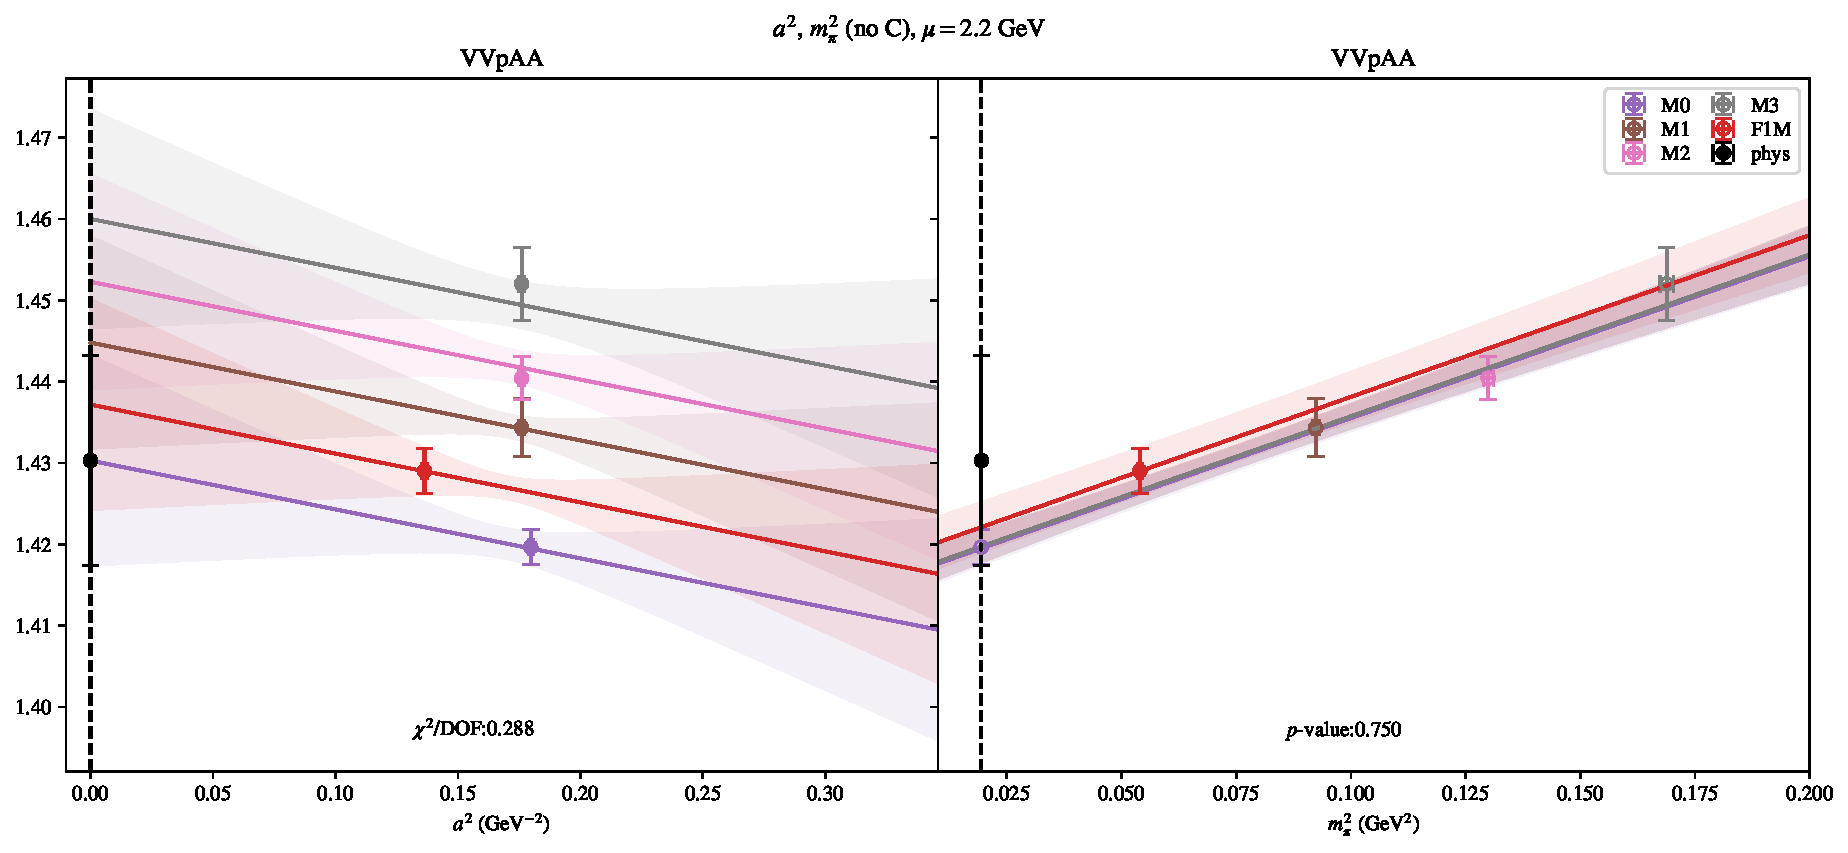
\includepdf[link, pages=-]{VVpAA/NPR/bag_a2m2noC_22.pdf}
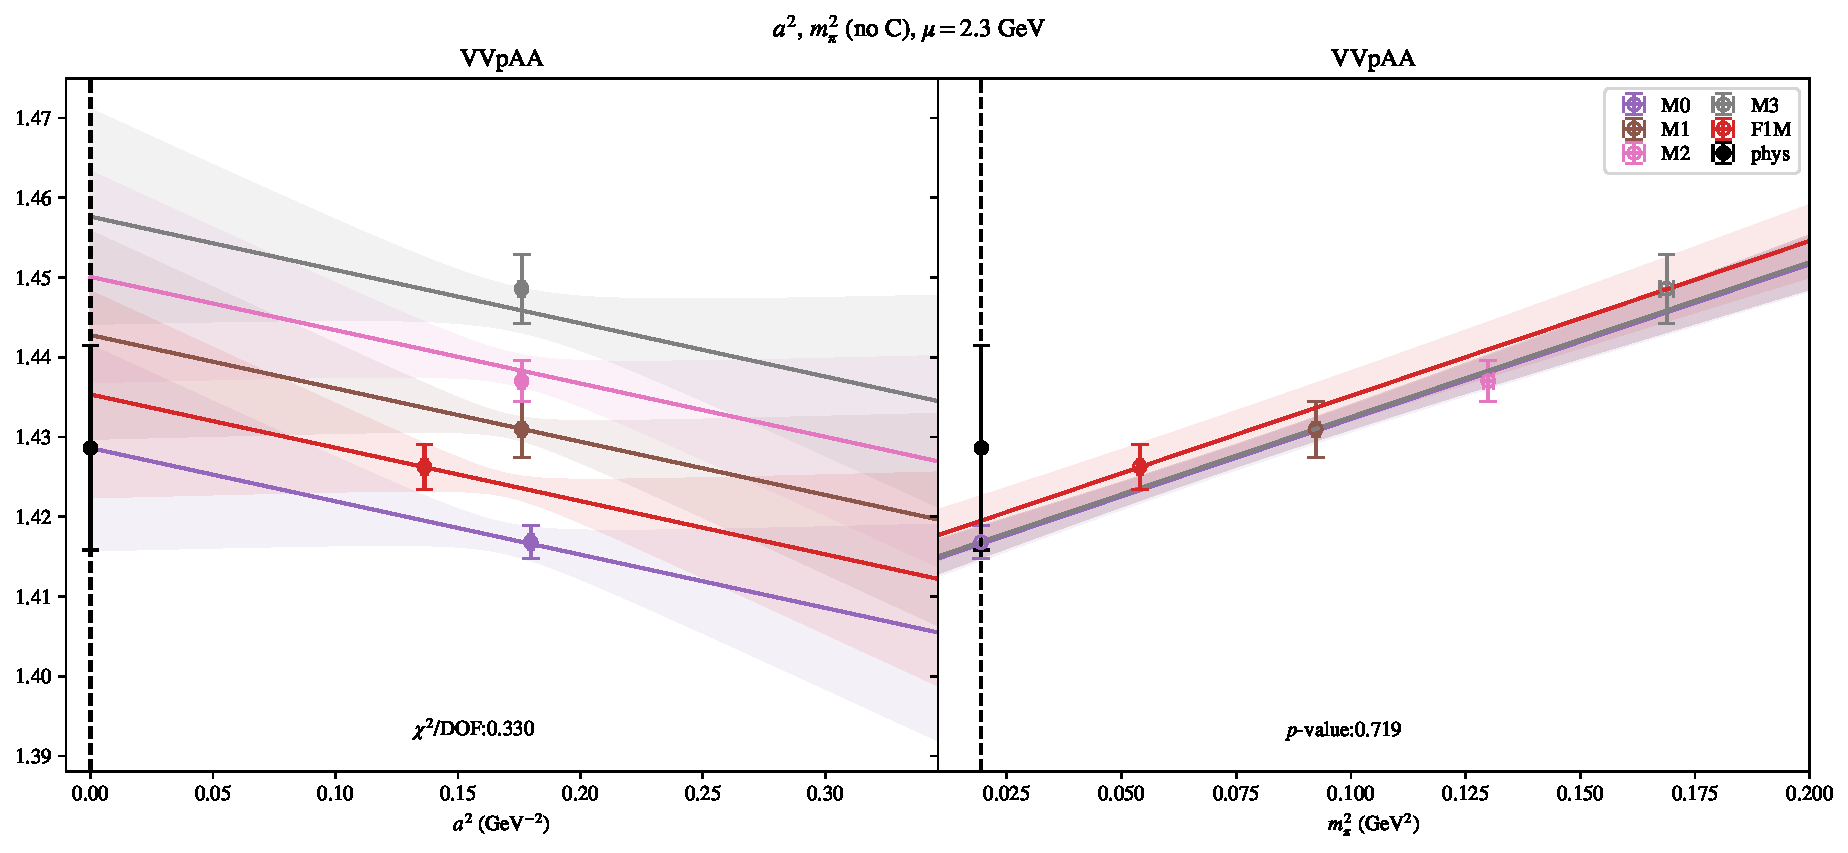
\includepdf[link, pages=-]{VVpAA/NPR/bag_a2m2noC_23.pdf}
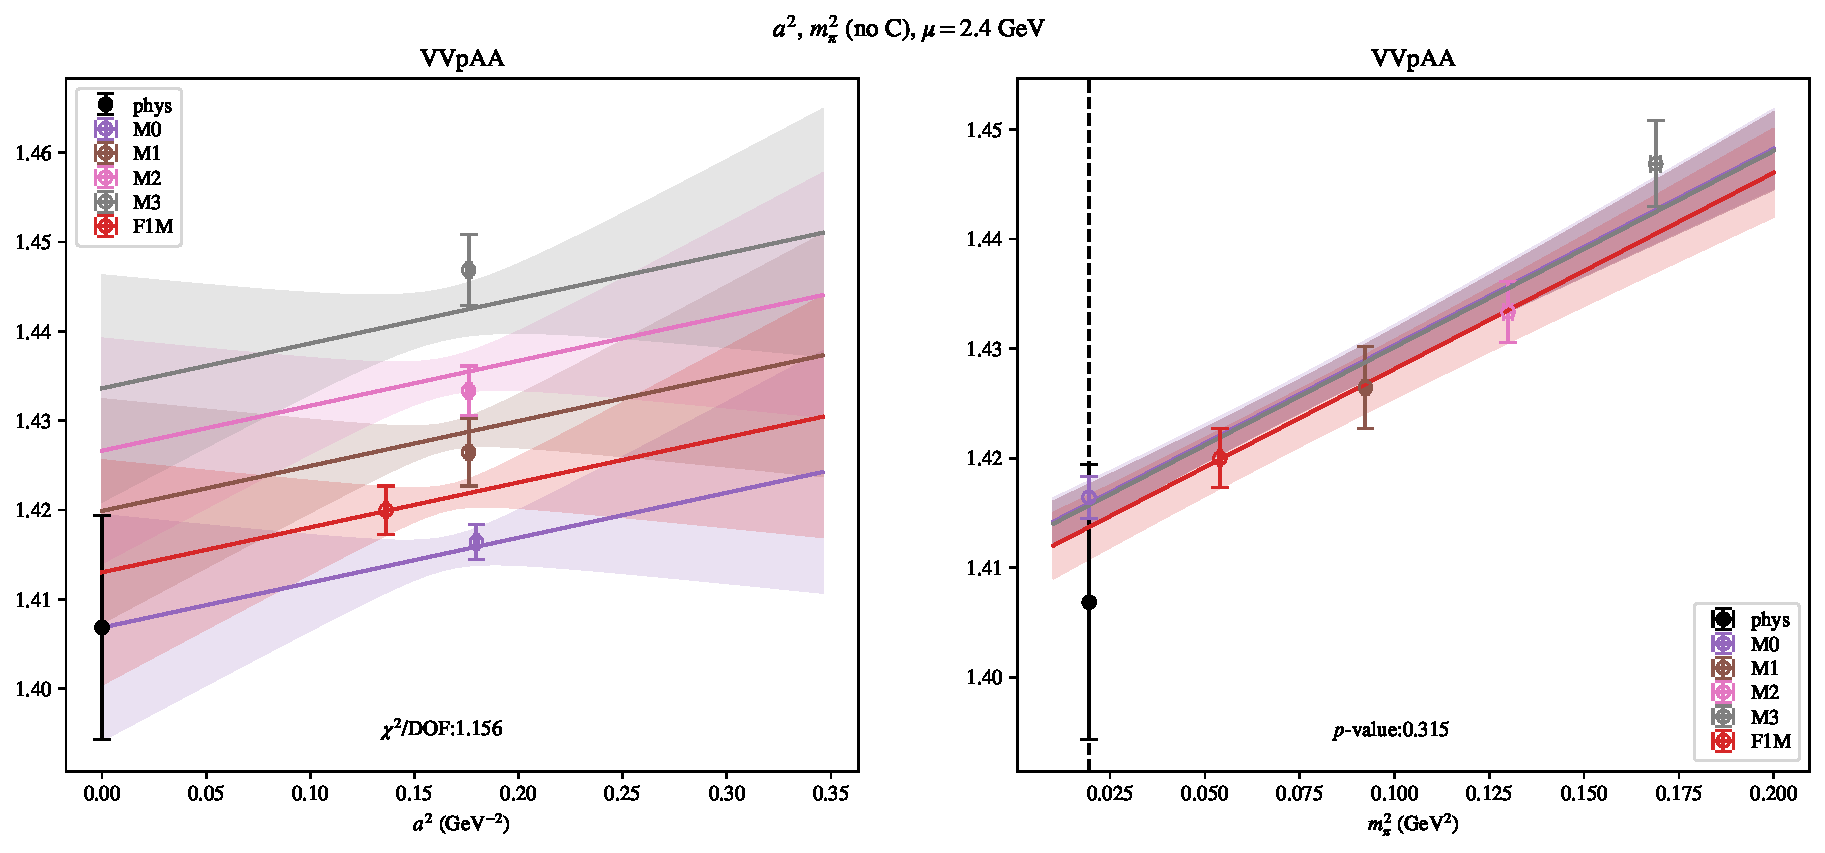
\includepdf[link, pages=-]{VVpAA/NPR/bag_a2m2noC_24.pdf}
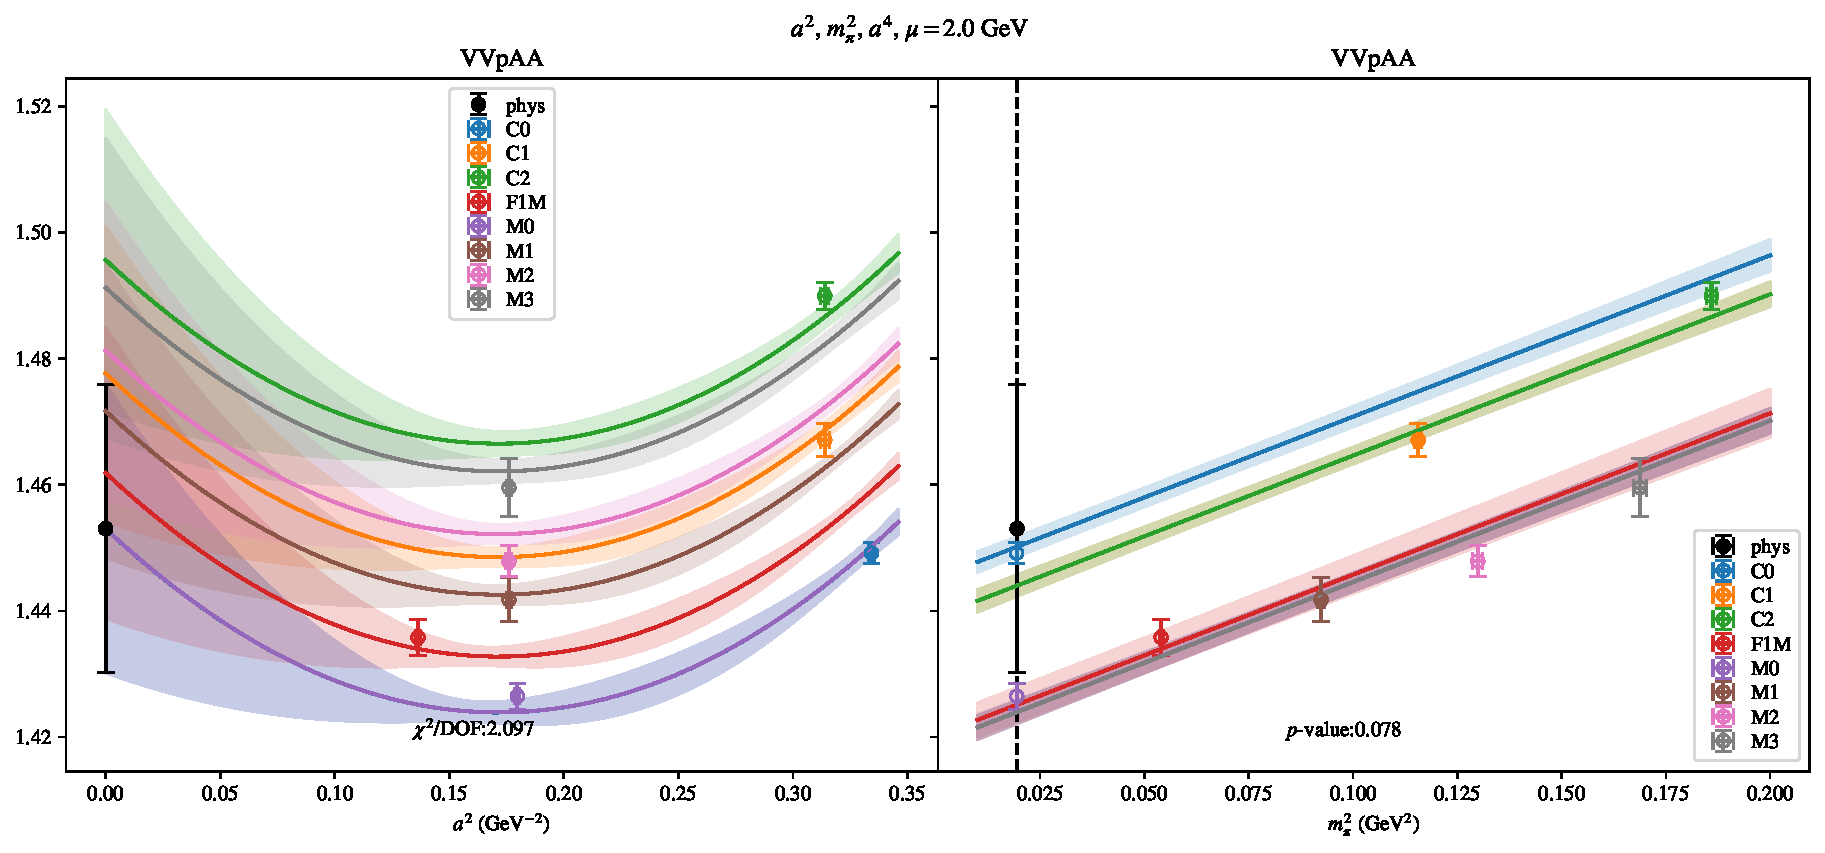
\includepdf[link, pages=-]{VVpAA/NPR/bag_a2a4m2_20.pdf}
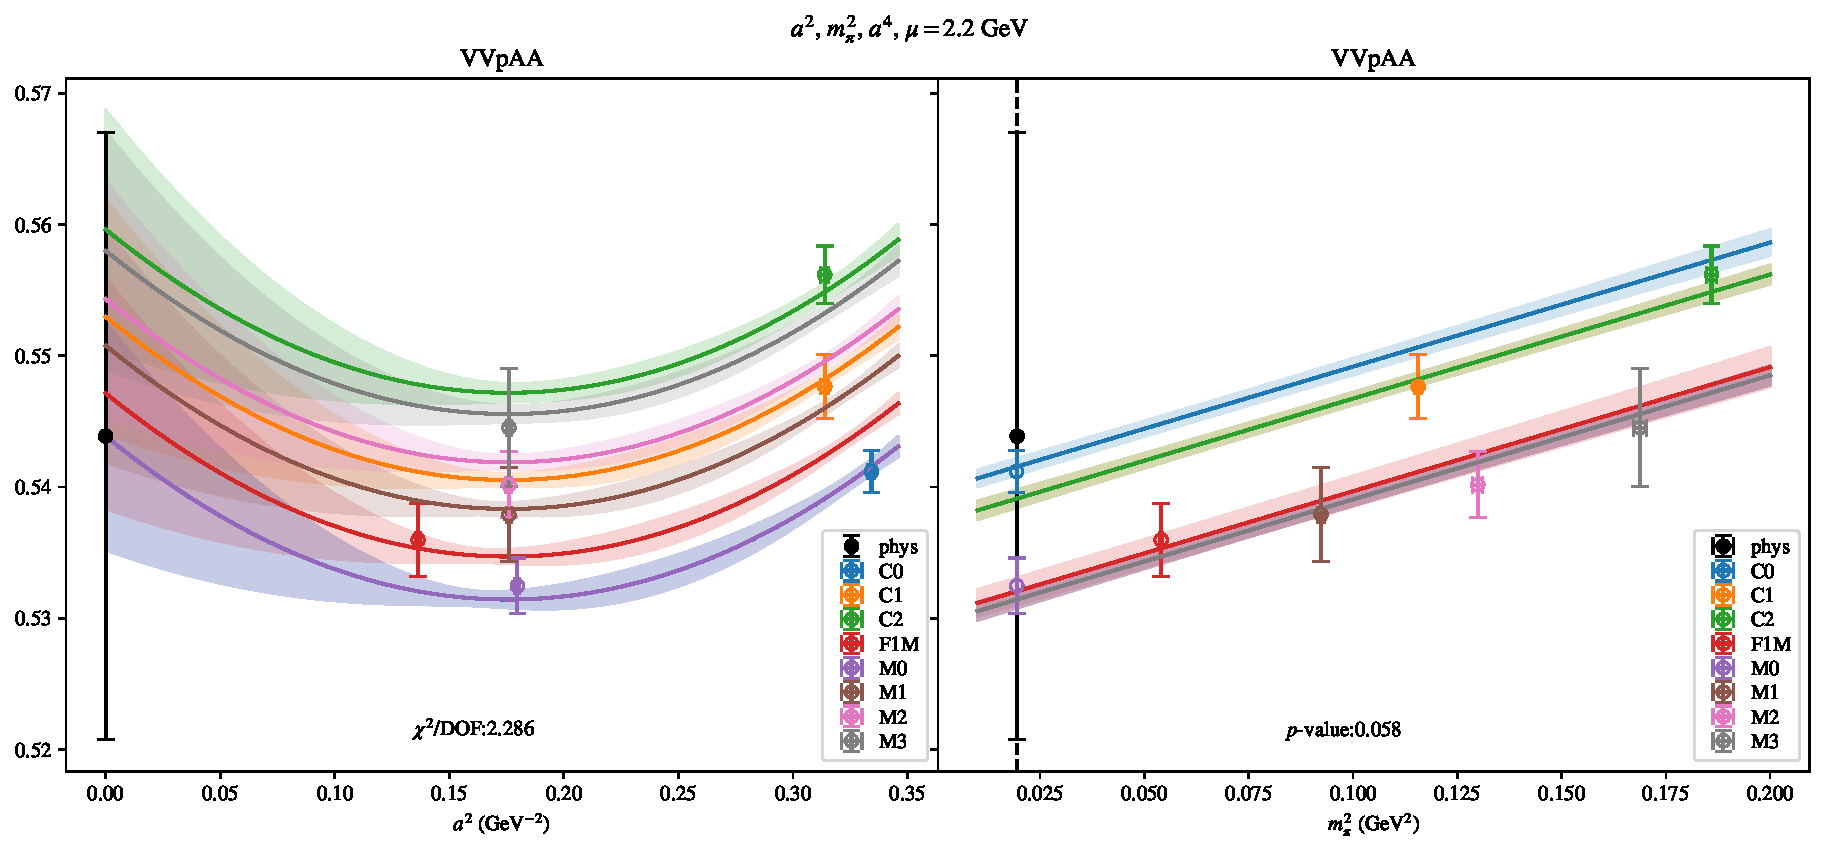
\includepdf[link, pages=-]{VVpAA/NPR/bag_a2a4m2_22.pdf}
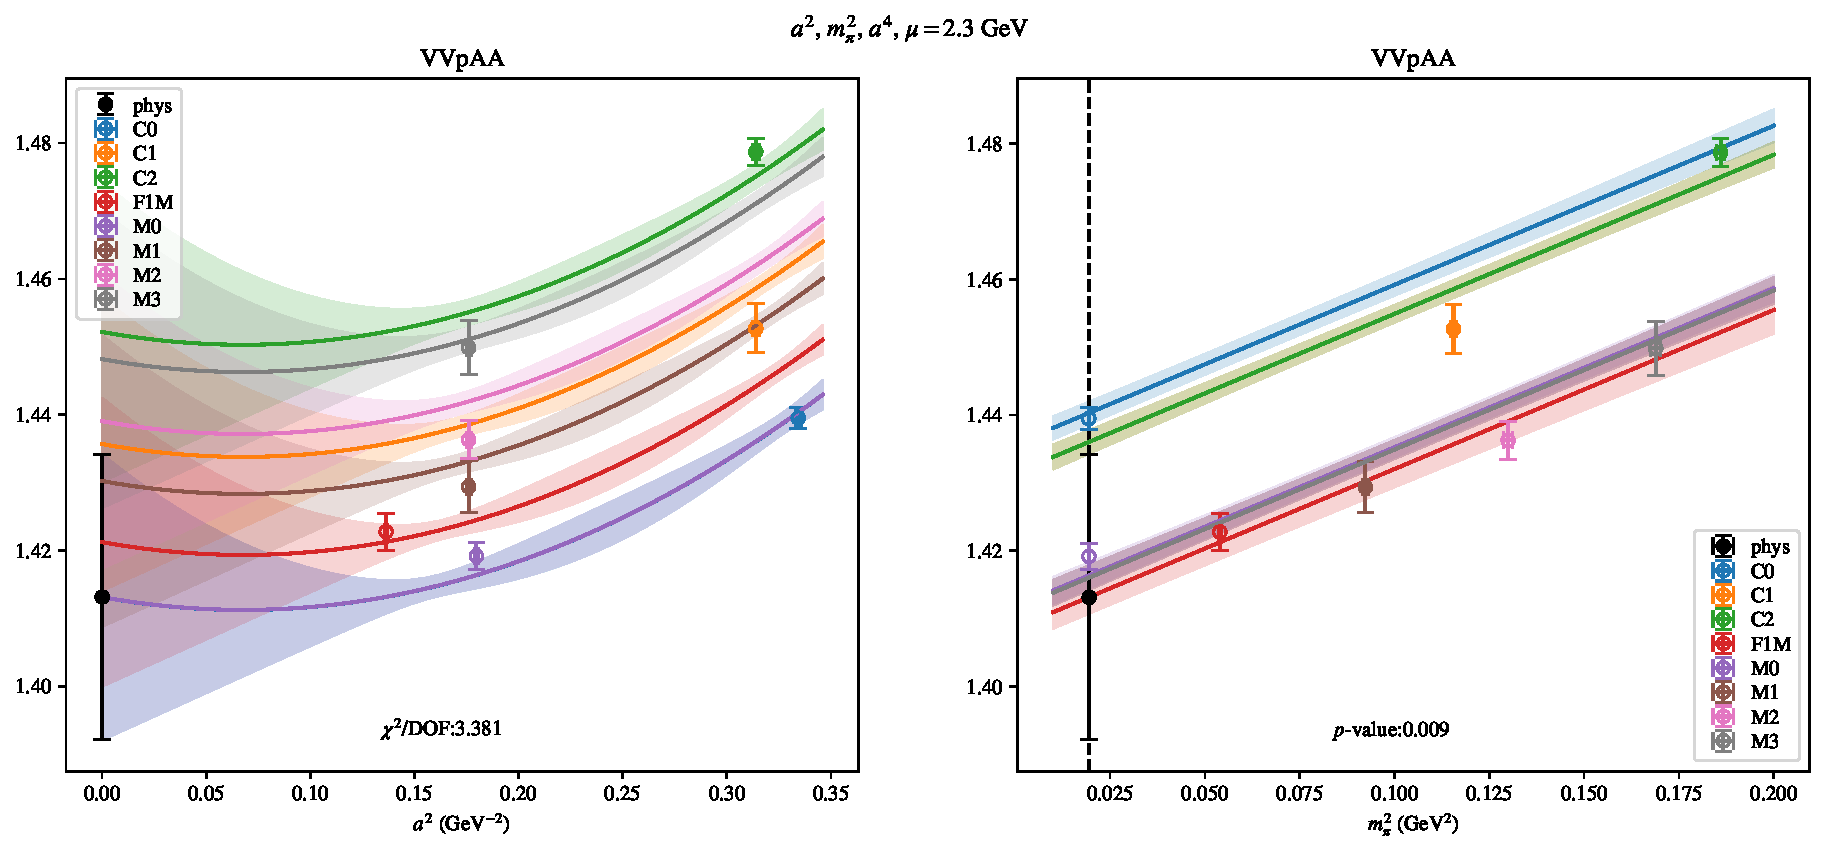
\includepdf[link, pages=-]{VVpAA/NPR/bag_a2a4m2_23.pdf}
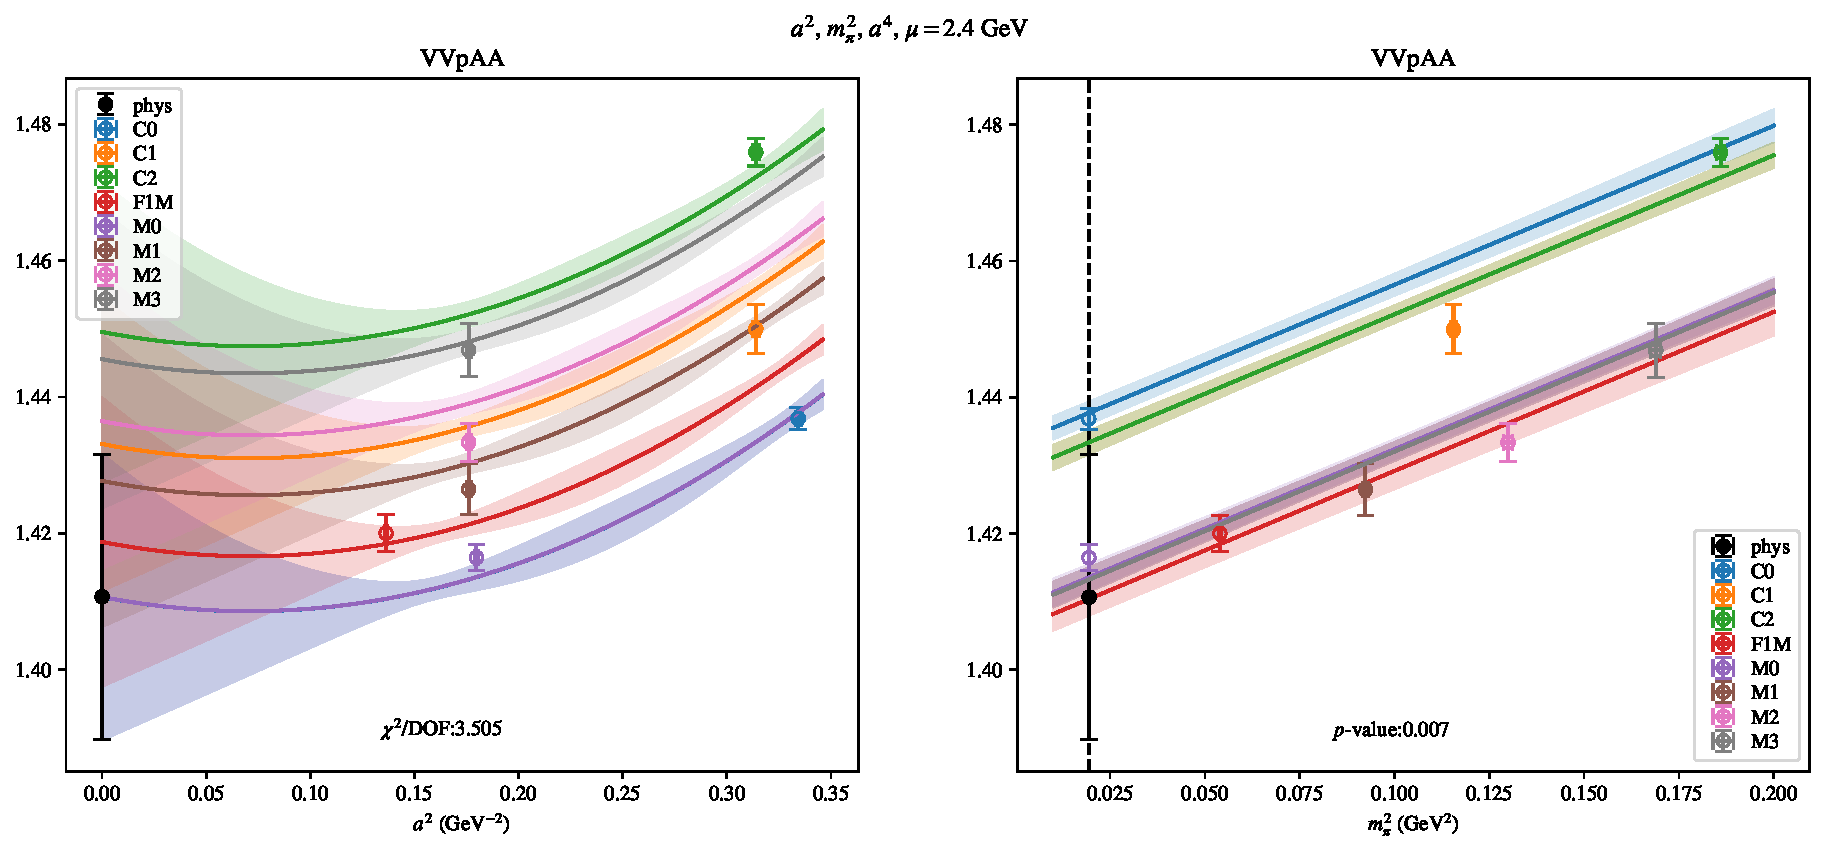
\includepdf[link, pages=-]{VVpAA/NPR/bag_a2a4m2_24.pdf}
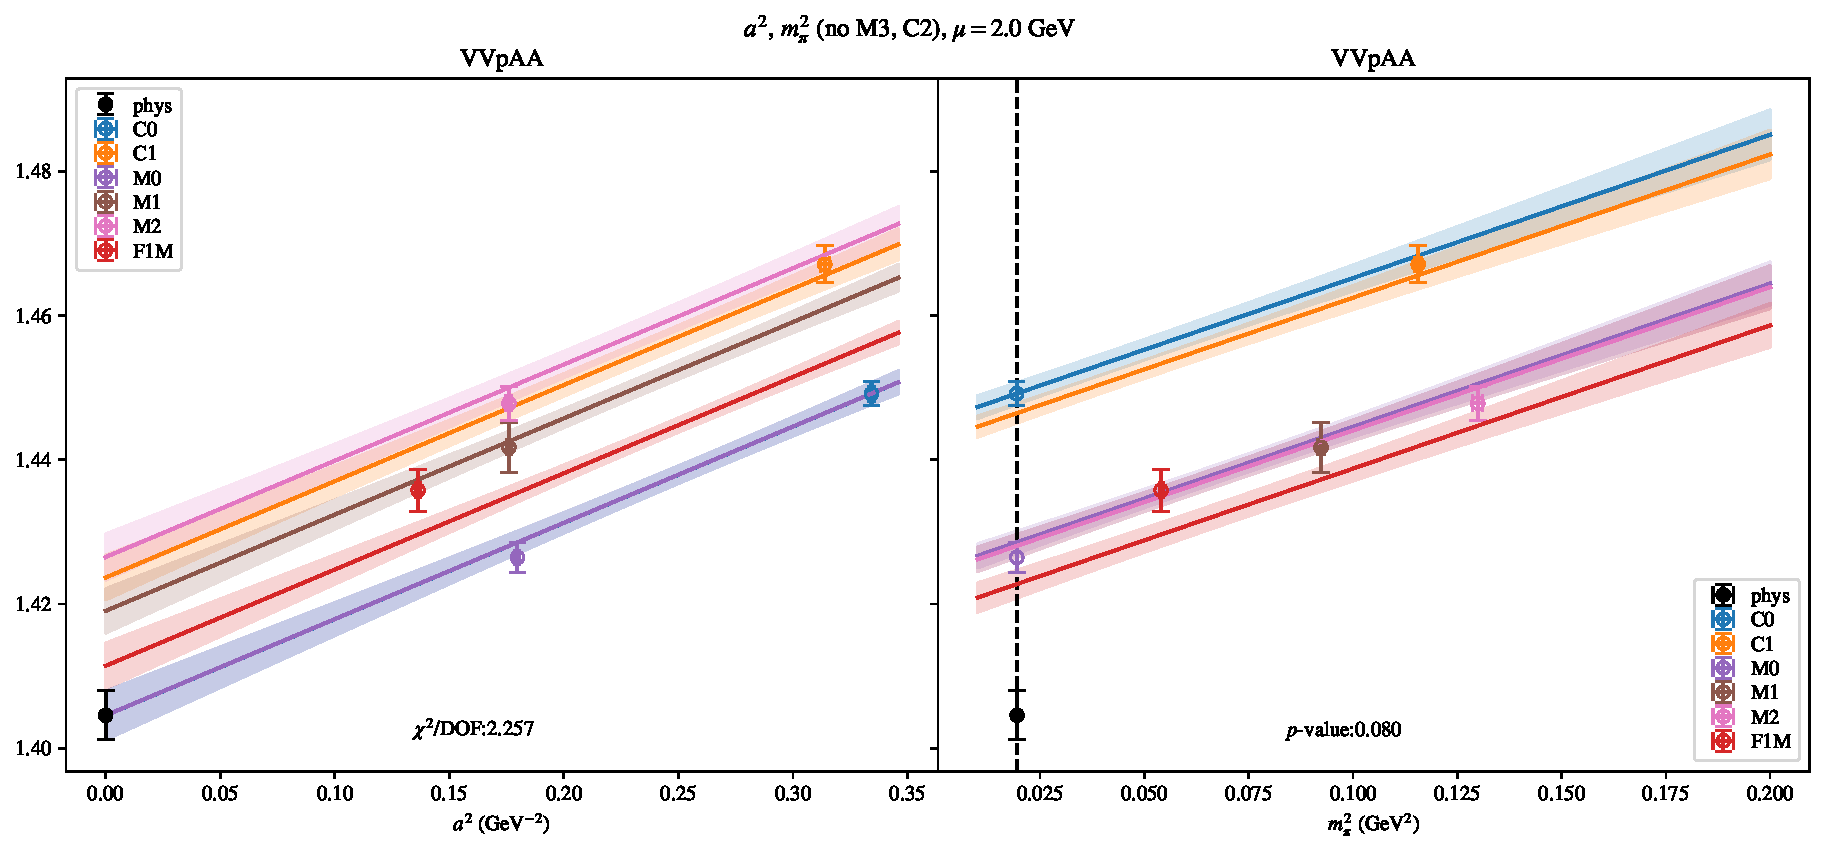
\includepdf[link, pages=-]{VVpAA/NPR/bag_a2m2mcut_20.pdf}
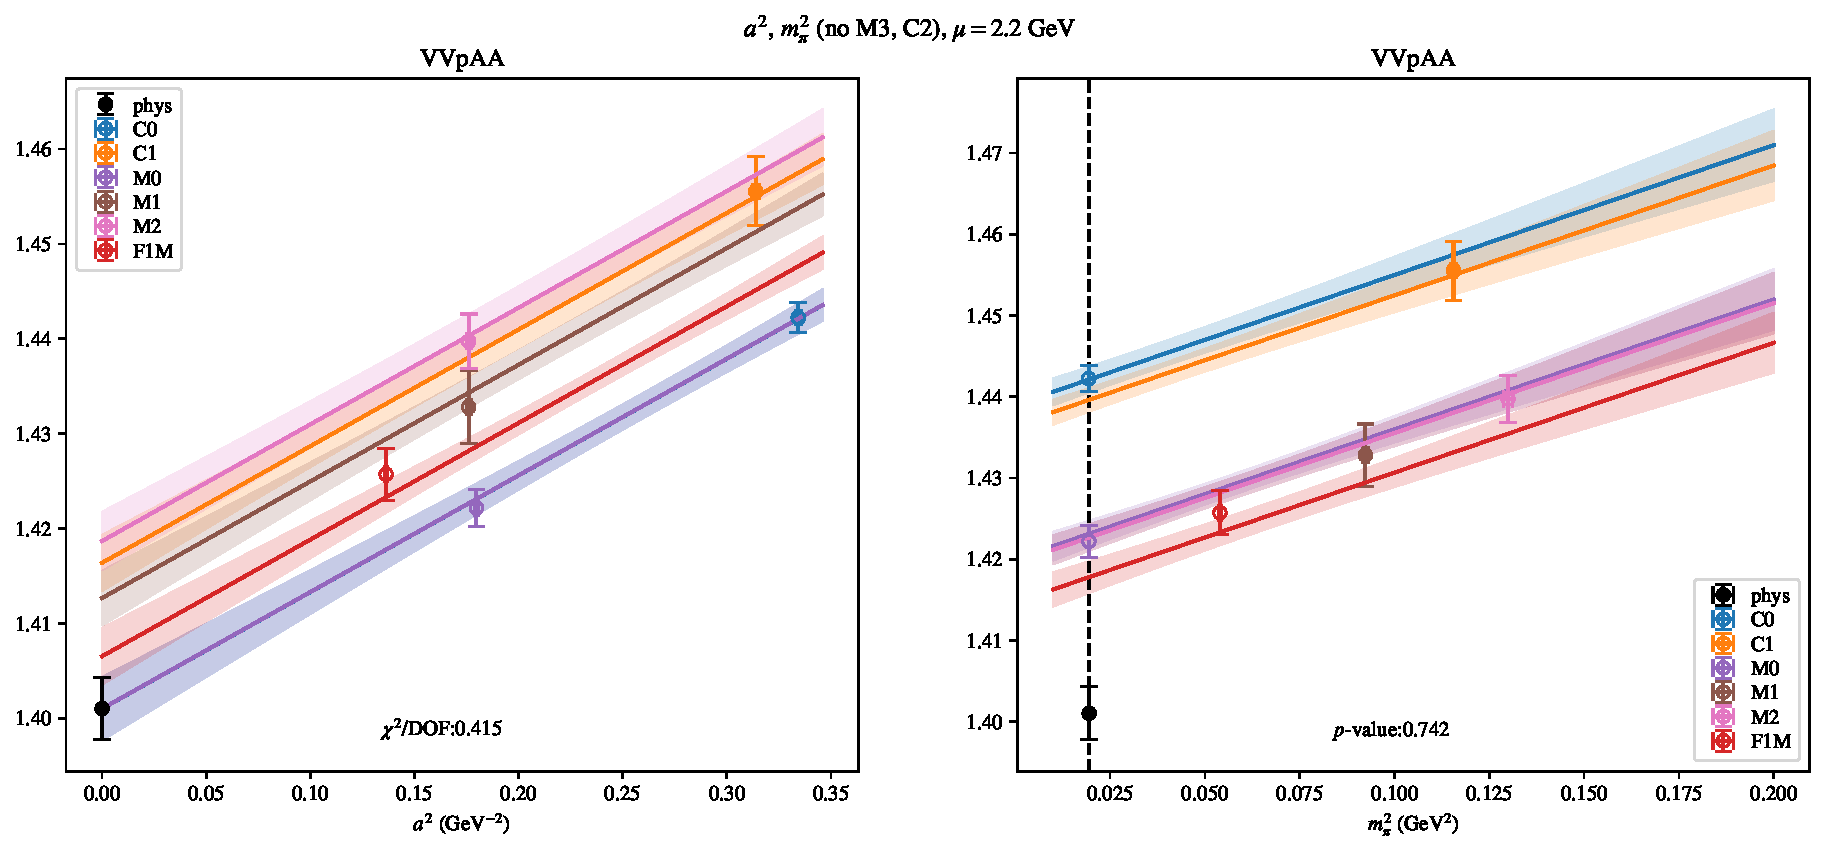
\includepdf[link, pages=-]{VVpAA/NPR/bag_a2m2mcut_22.pdf}
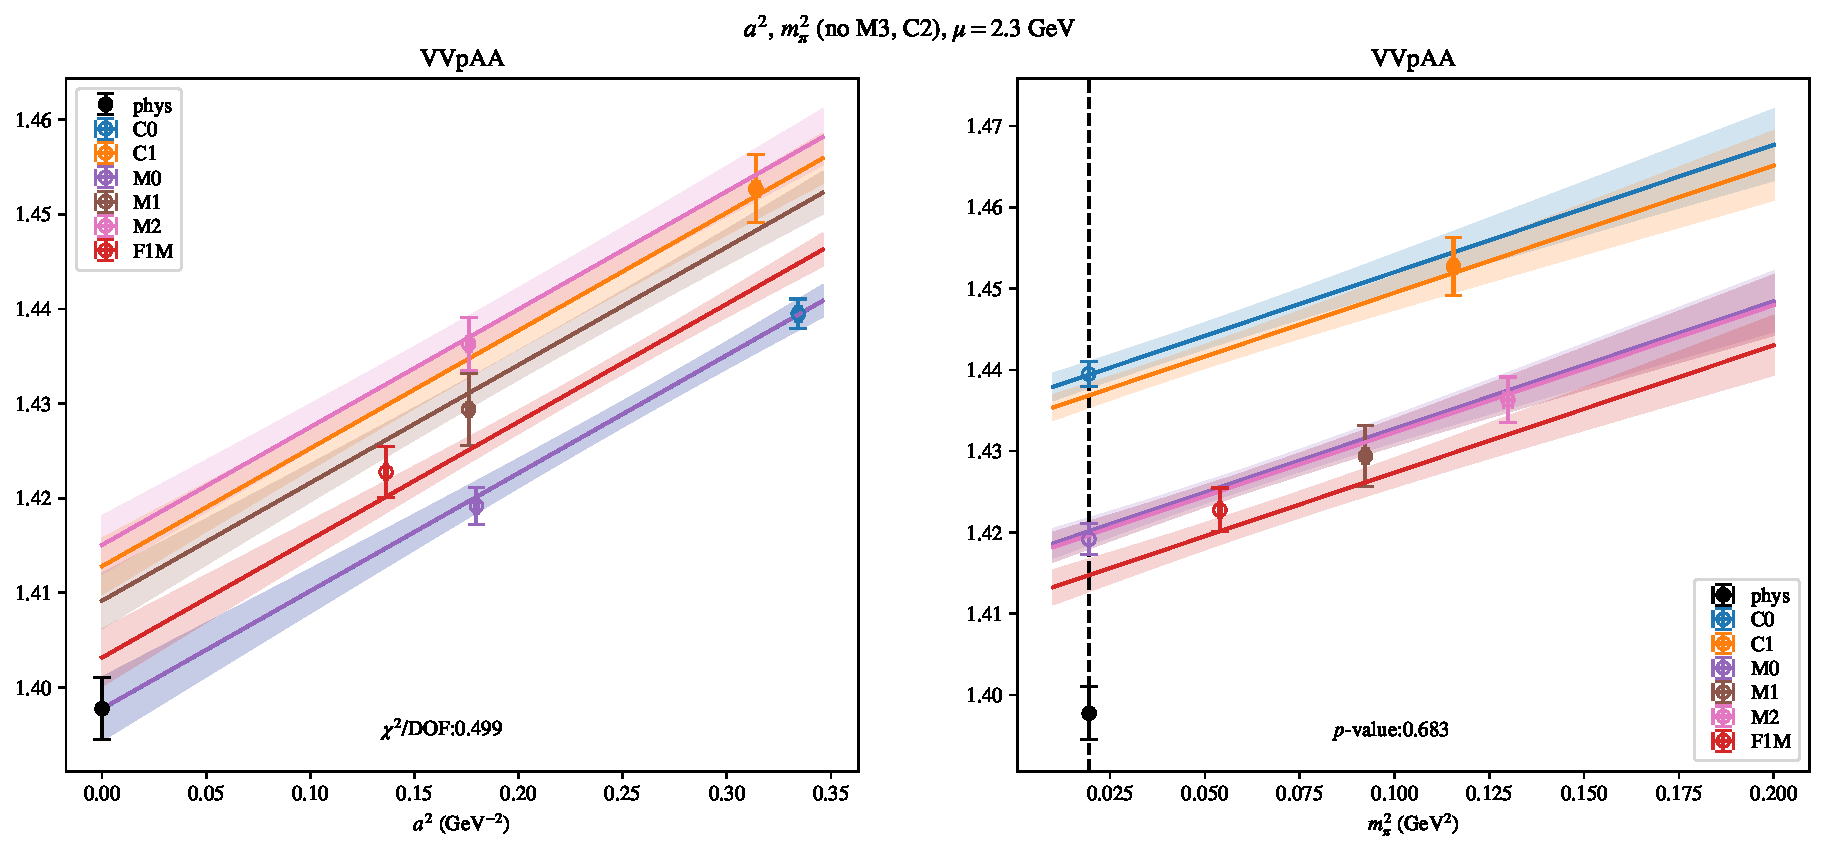
\includepdf[link, pages=-]{VVpAA/NPR/bag_a2m2mcut_23.pdf}
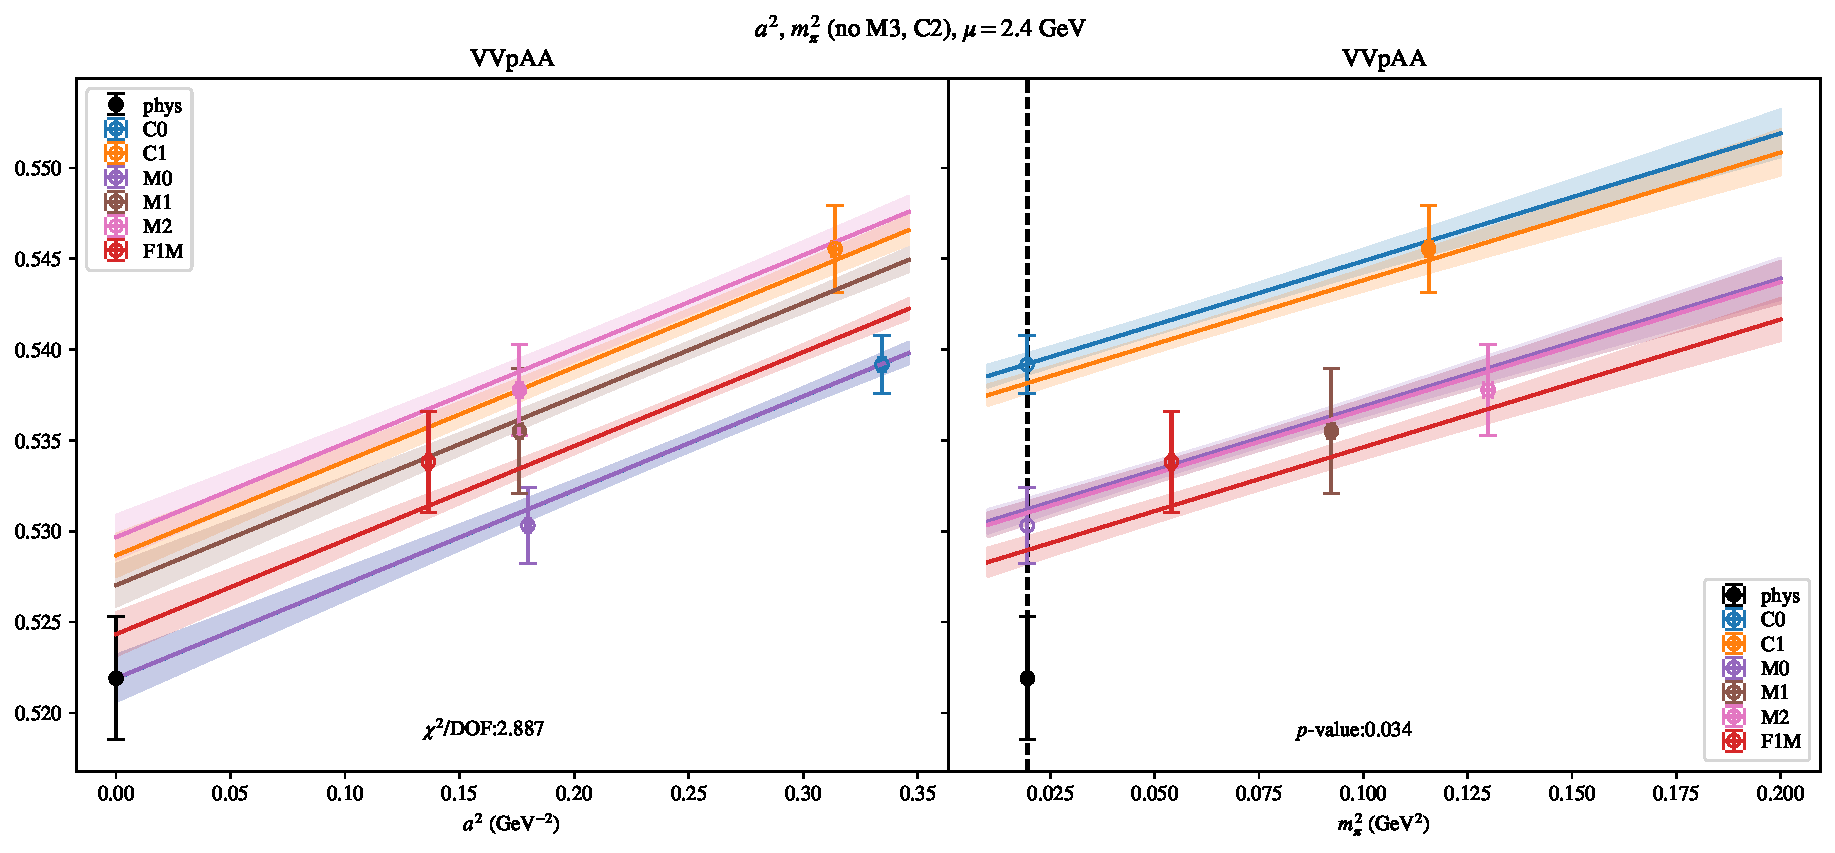
\includepdf[link, pages=-]{VVpAA/NPR/bag_a2m2mcut_24.pdf}
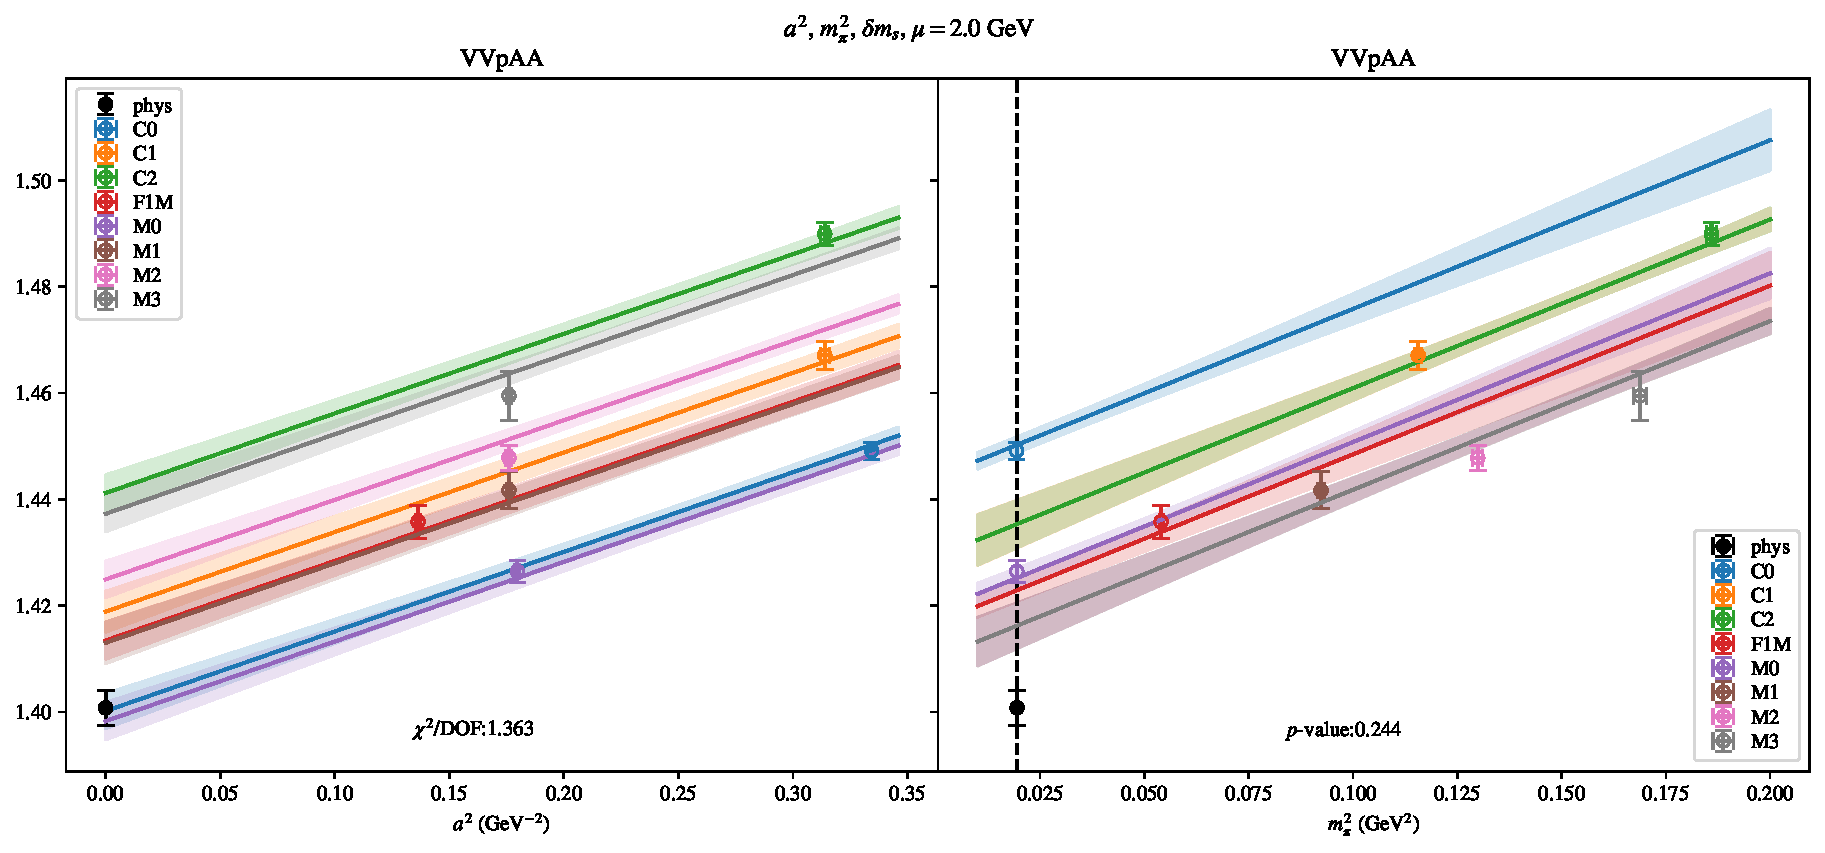
\includepdf[link, pages=-]{VVpAA/NPR/bag_a2m2delm_20.pdf}
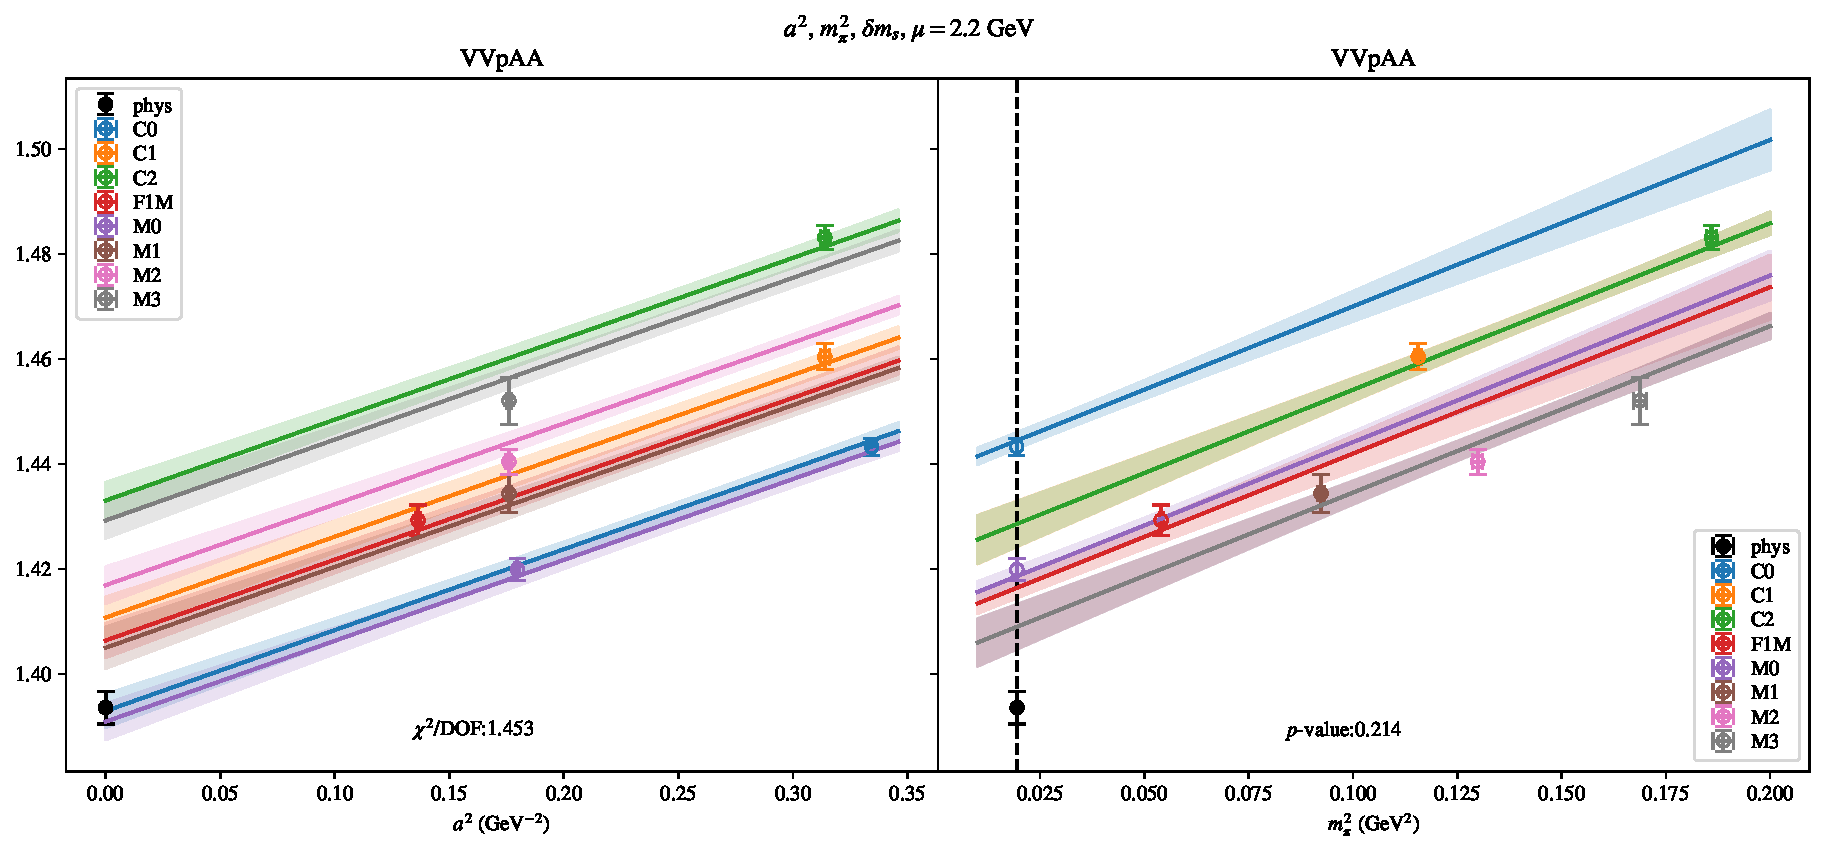
\includepdf[link, pages=-]{VVpAA/NPR/bag_a2m2delm_22.pdf}
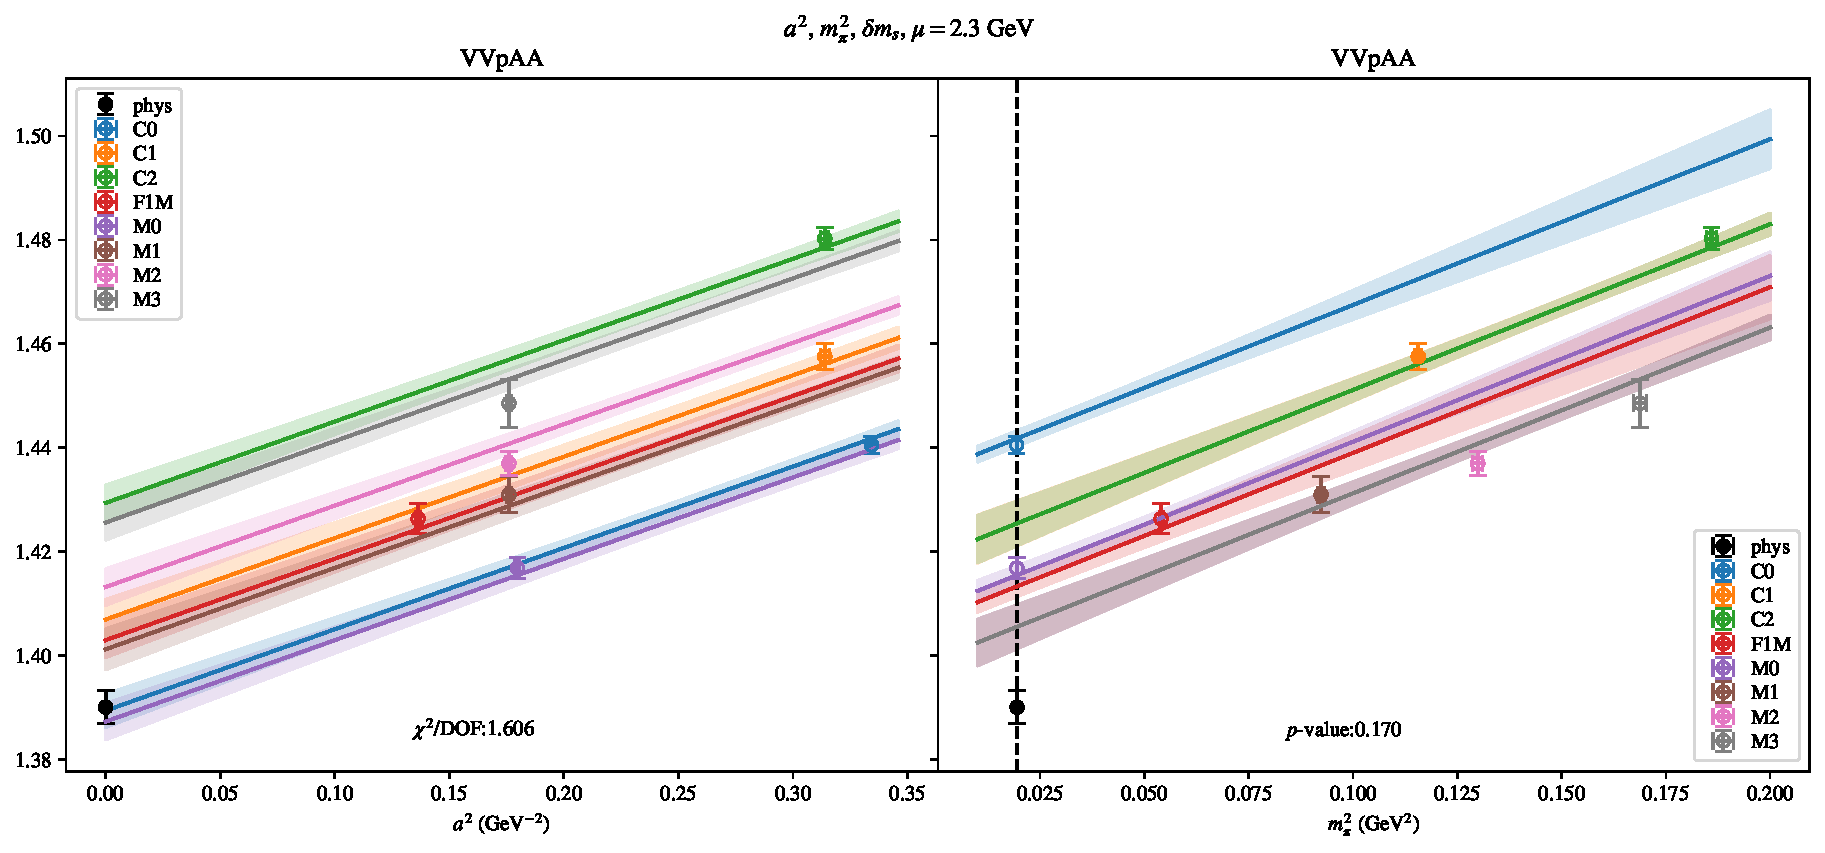
\includepdf[link, pages=-]{VVpAA/NPR/bag_a2m2delm_23.pdf}
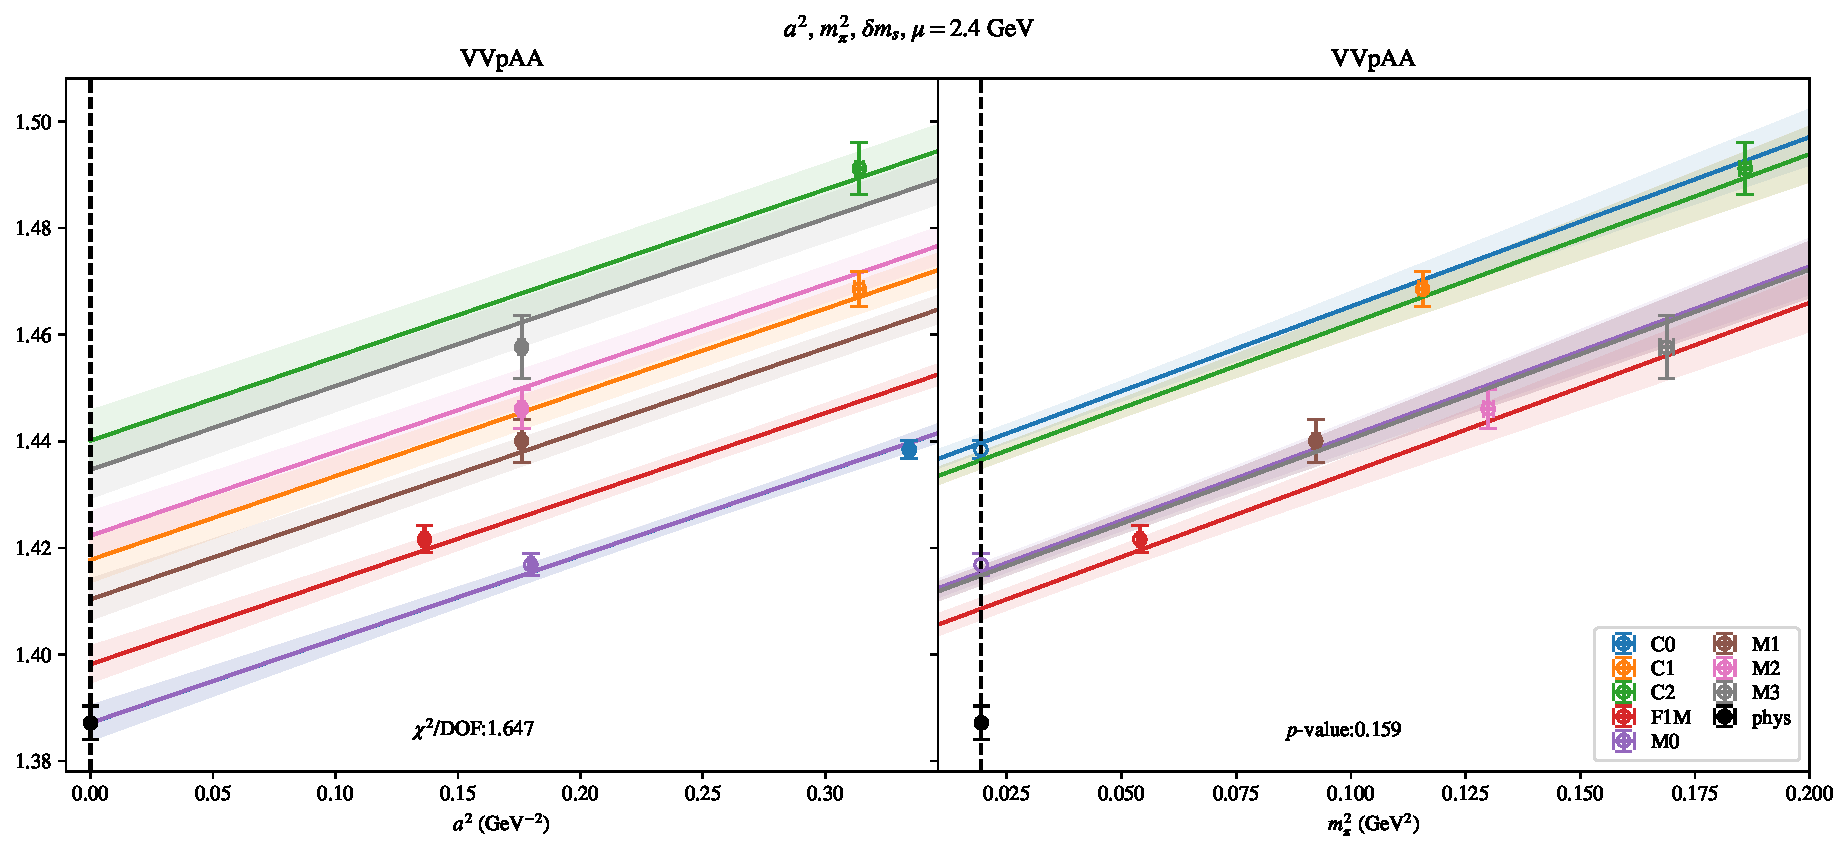
\includepdf[link, pages=-]{VVpAA/NPR/bag_a2m2delm_24.pdf}
\clearpage
\section{$\mathcal{B}_2$}
\begin{table}[h!]
\begin{center}
\begin{tabular}{|c|c|c|c|c|c|}
\hline
$\mu$ (GeV) & $a^2$, $m_\pi^2$& $a^2$, $m_\pi^2$ (no C)& $a^2$, $m_\pi^2$, $a^4$& $a^2$, $m_\pi^2$ (no M3, C2)& $a^2$, $m_\pi^2$, $\delta m_s$\\
\hline
2.0& \hyperlink{VVmAA/NPR/bag_a2m2_20.pdf.1}{\textbf{-0.987(11)}: 0.172 (0.973)} & \hyperlink{VVmAA/NPR/bag_a2m2noC_20.pdf.1}{\textbf{-0.942(57)}: 0.002 (0.998)} & \hyperlink{VVmAA/NPR/bag_a2a4m2_20.pdf.1}{\textbf{-0.919(91)}: 0.037 (0.997)} & \hyperlink{VVmAA/NPR/bag_a2m2mcut_20.pdf.1}{\textbf{-0.987(12)}: 0.233 (0.873)} & \hyperlink{VVmAA/NPR/bag_a2m2delm_20.pdf.1}{\textbf{-0.987(12)}: 0.086 (0.987)}\\
2.2& \hyperlink{VVmAA/NPR/bag_a2m2_22.pdf.1}{\textbf{-1.000(10)}: 0.183 (0.969)} & \hyperlink{VVmAA/NPR/bag_a2m2noC_22.pdf.1}{\textbf{-0.962(46)}: 0.008 (0.992)} & \hyperlink{VVmAA/NPR/bag_a2a4m2_22.pdf.1}{\textbf{-0.938(73)}: 0.031 (0.998)} & \hyperlink{VVmAA/NPR/bag_a2m2mcut_22.pdf.1}{\textbf{-1.002(10)}: 0.29 (0.833)} & \hyperlink{VVmAA/NPR/bag_a2m2delm_22.pdf.1}{\textbf{-1.000(10)}: 0.121 (0.975)}\\
2.3& \hyperlink{VVmAA/NPR/bag_a2m2_23.pdf.1}{\textbf{-1.0071(92)}: 0.242 (0.944)} & \hyperlink{VVmAA/NPR/bag_a2m2noC_23.pdf.1}{\textbf{-0.968(43)}: 0.008 (0.992)} & \hyperlink{VVmAA/NPR/bag_a2a4m2_23.pdf.1}{\textbf{-0.940(68)}: 0.021 (0.999)} & \hyperlink{VVmAA/NPR/bag_a2m2mcut_23.pdf.1}{\textbf{-1.0082(98)}: 0.35 (0.789)} & \hyperlink{VVmAA/NPR/bag_a2m2delm_23.pdf.1}{\textbf{-1.0068(95)}: 0.12 (0.975)}\\
2.4& \hyperlink{VVmAA/NPR/bag_a2m2_24.pdf.1}{\textbf{-1.0109(88)}: 0.253 (0.938)} & \hyperlink{VVmAA/NPR/bag_a2m2noC_24.pdf.1}{\textbf{-0.975(36)}: 0.009 (0.991)} & \hyperlink{VVmAA/NPR/bag_a2a4m2_24.pdf.1}{\textbf{-0.949(61)}: 0.027 (0.999)} & \hyperlink{VVmAA/NPR/bag_a2m2mcut_24.pdf.1}{\textbf{-1.0118(91)}: 0.398 (0.754)} & \hyperlink{VVmAA/NPR/bag_a2m2delm_24.pdf.1}{\textbf{-1.0115(83)}: 0.142 (0.966)}\\
\hline
\end{tabular}
\caption{Physical point value from chiral and continuum extrapolation at renormalisation scale $\mu$. Entries are \textbf{value(error)}: $\chi^2/\text{DOF}$ ($p$-value).}
\end{center}
\end{table}
\begin{table}[h!]
\begin{center}
\begin{tabular}{|c c|c|c|c|c|c|}
\hline
$\mu$ (GeV) &  & $a^2$, $m_\pi^2$& $a^2$, $m_\pi^2$ (no C)& $a^2$, $m_\pi^2$, $a^4$& $a^2$, $m_\pi^2$ (no M3, C2)& $a^2$, $m_\pi^2$, $\delta m_s$\\
\hline
\multirow{3}{0.5in}{2.0} & $\alpha$ & 0.160(43)& -0.11(32)& -0.46(82)& 0.161(46)& 0.163(44)\\
 & $\beta$ & -0.0019(11)& -0.0023(22)& -0.0016(13)& -0.0015(21)& -0.0005(26)\\
 & $\gamma$ &  &  & 1.2(16)&  & -0.054(94)\\
\hline
\multirow{3}{0.5in}{2.2} & $\alpha$ & 0.205(37)& -0.03(26)& -0.37(66)& 0.209(37)& 0.209(37)\\
 & $\beta$ & -0.0016(10)& -0.0017(17)& -0.0014(10)& -0.0011(16)& -0.0004(20)\\
 & $\gamma$ &  &  & 1.2(13)&  & -0.045(71)\\
\hline
\multirow{3}{0.5in}{2.3} & $\alpha$ & 0.232(34)& -0.004(248)& -0.38(60)& 0.235(35)& 0.235(34)\\
 & $\beta$ & -0.00169(91)& -0.0017(16)& -0.00148(95)& -0.0013(16)& -0.0004(19)\\
 & $\gamma$ &  &  & 1.2(12)&  & -0.051(69)\\
\hline
\multirow{3}{0.5in}{2.4} & $\alpha$ & 0.251(31)& 0.03(21)& -0.32(55)& 0.254(33)& 0.256(30)\\
 & $\beta$ & -0.00173(83)& -0.0017(13)& -0.00147(86)& -0.0014(13)& -0.0005(16)\\
 & $\gamma$ &  &  & 1.2(11)&  & -0.048(59)\\
\hline
\end{tabular}
\caption{Fit values of coefficients in $Q = Q_{phys} + \mathbf{\alpha} a^2 + \mathbf{\beta}\left(\frac{m_\pi^2}{f_\pi^2}-\frac{m_{\pi,PDG}^2}{f_\pi^2}\right) + \gamma(\ldots)$}
\end{center}
\end{table}
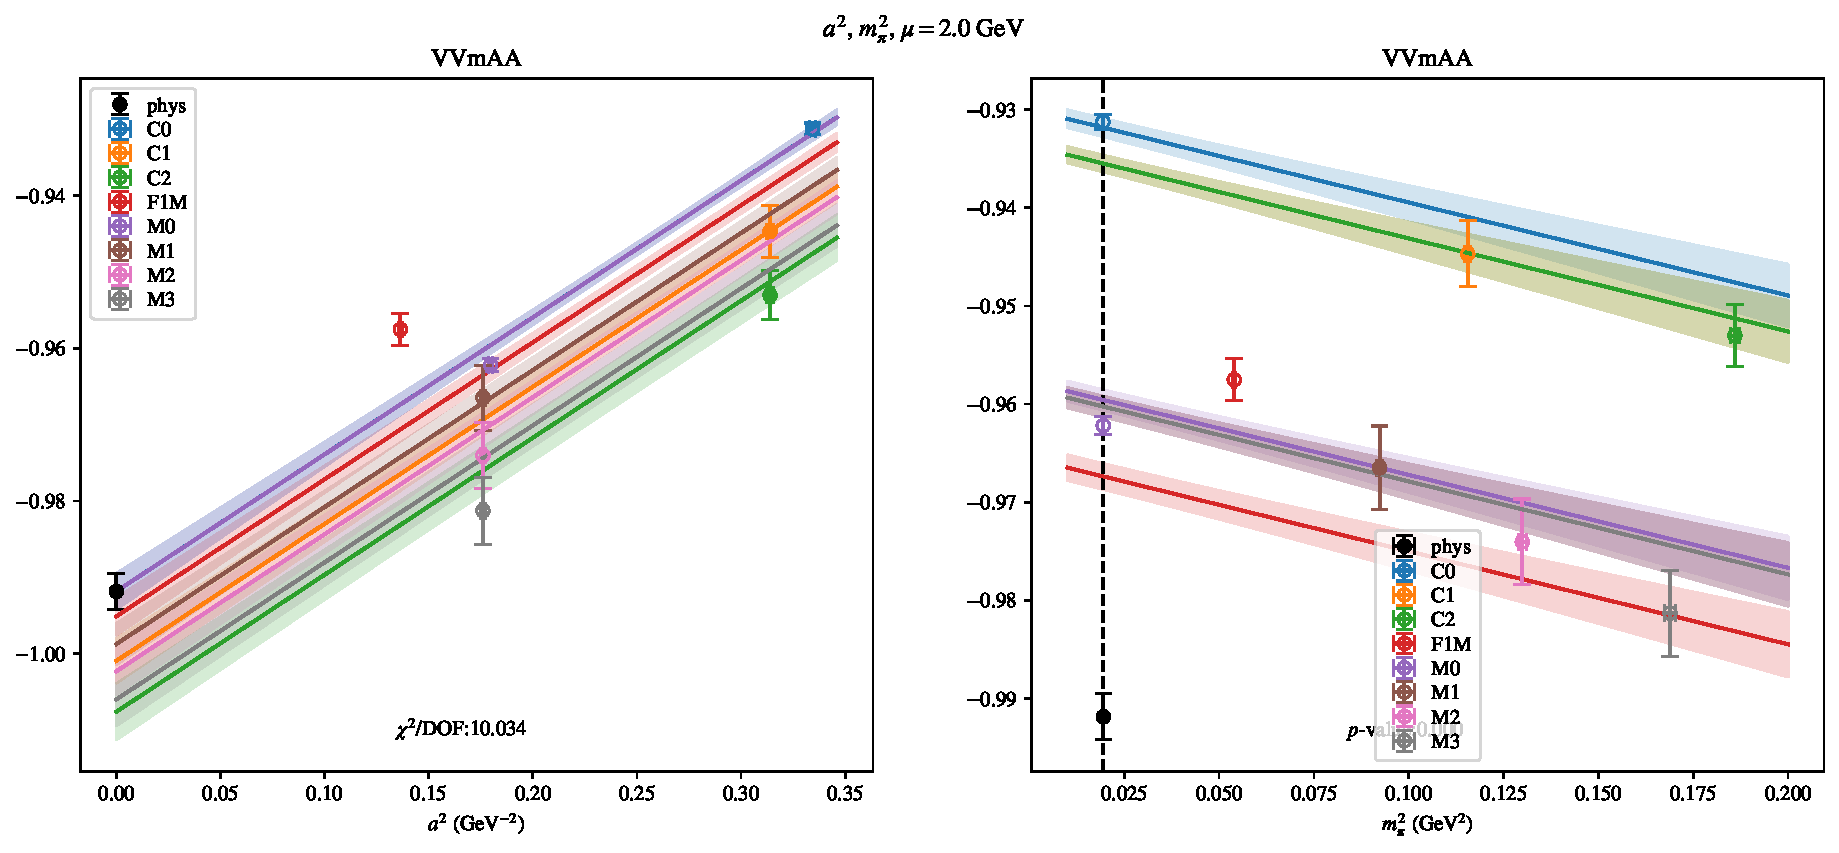
\includepdf[link, pages=-]{VVmAA/NPR/bag_a2m2_20.pdf}
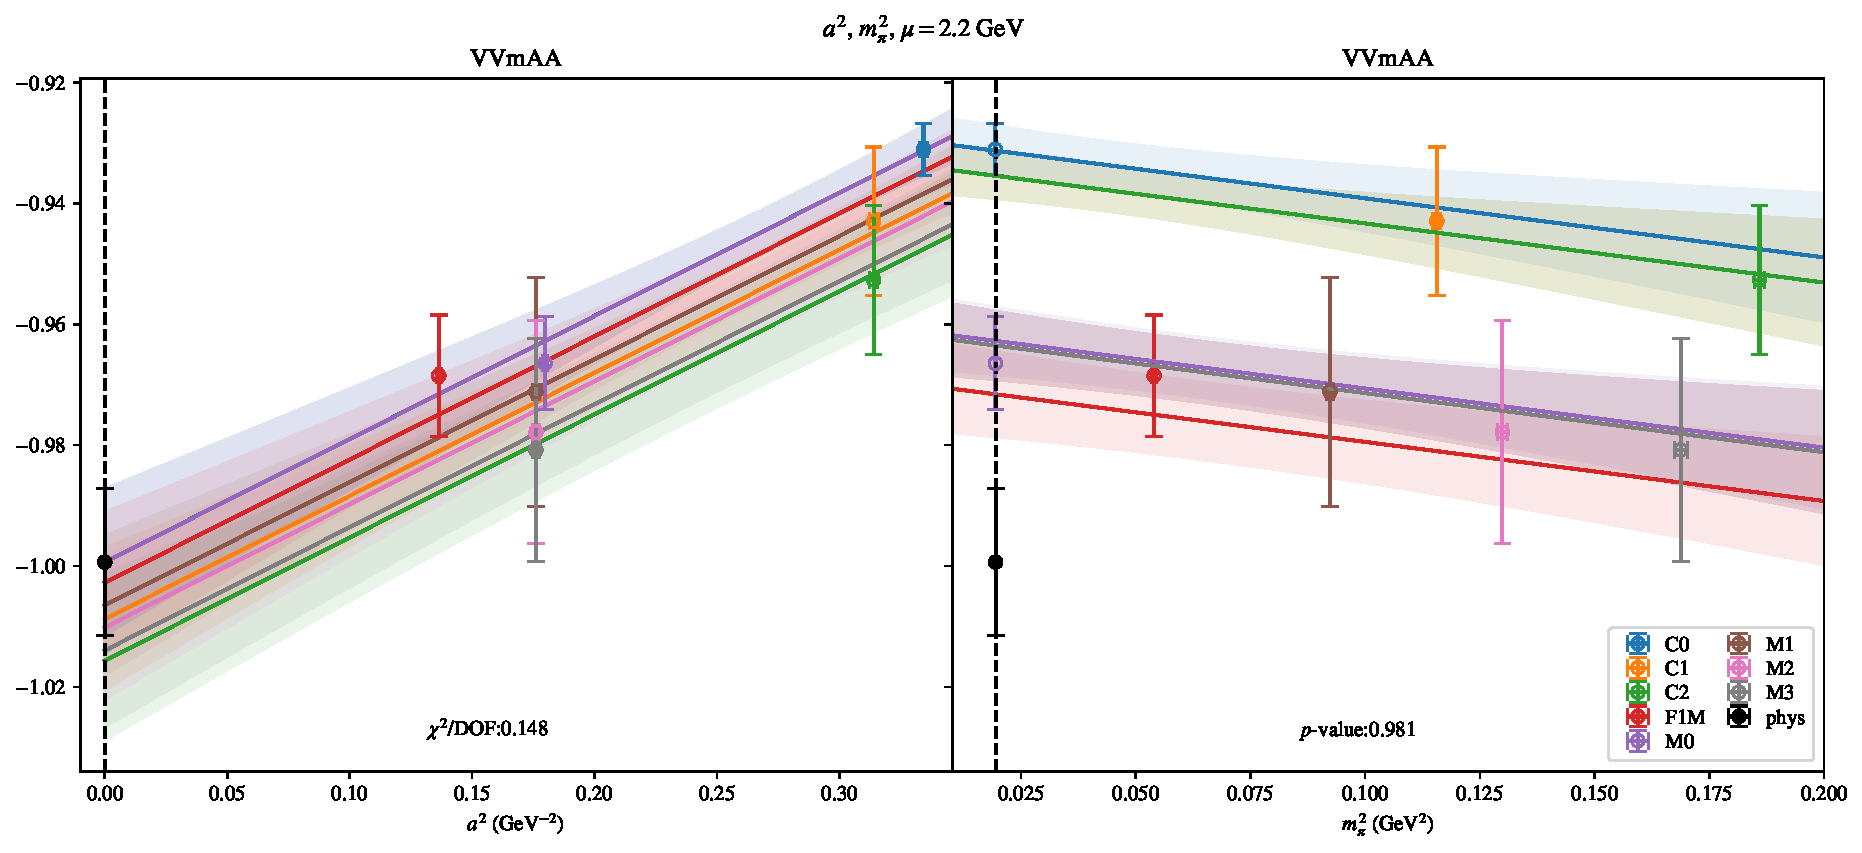
\includepdf[link, pages=-]{VVmAA/NPR/bag_a2m2_22.pdf}
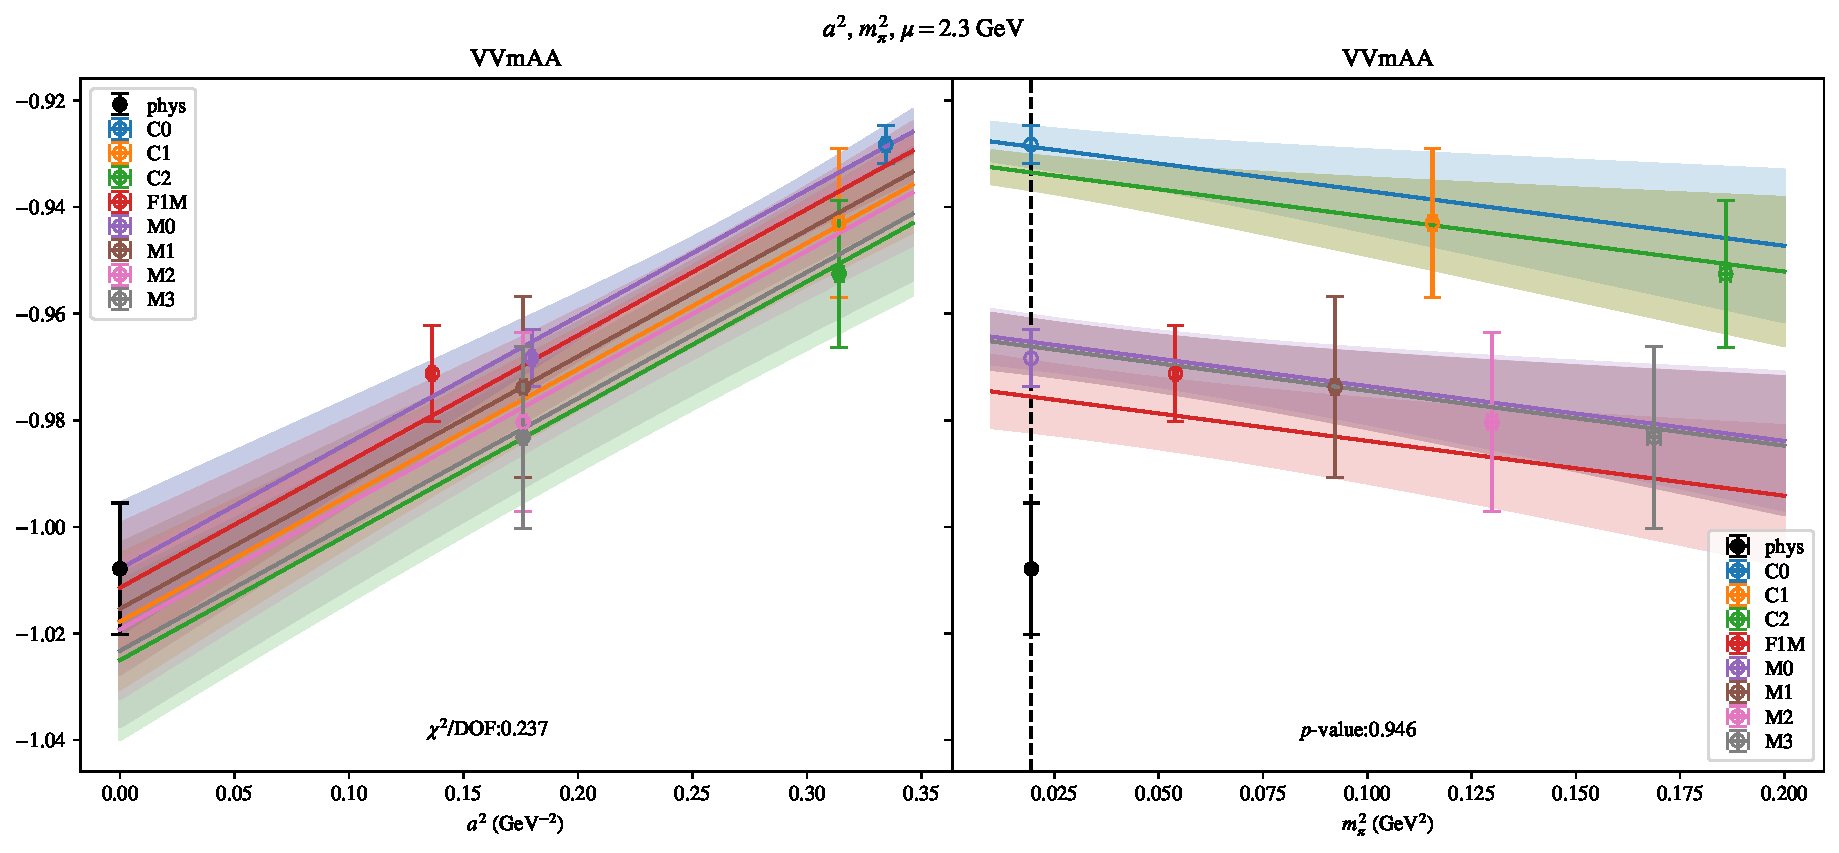
\includepdf[link, pages=-]{VVmAA/NPR/bag_a2m2_23.pdf}
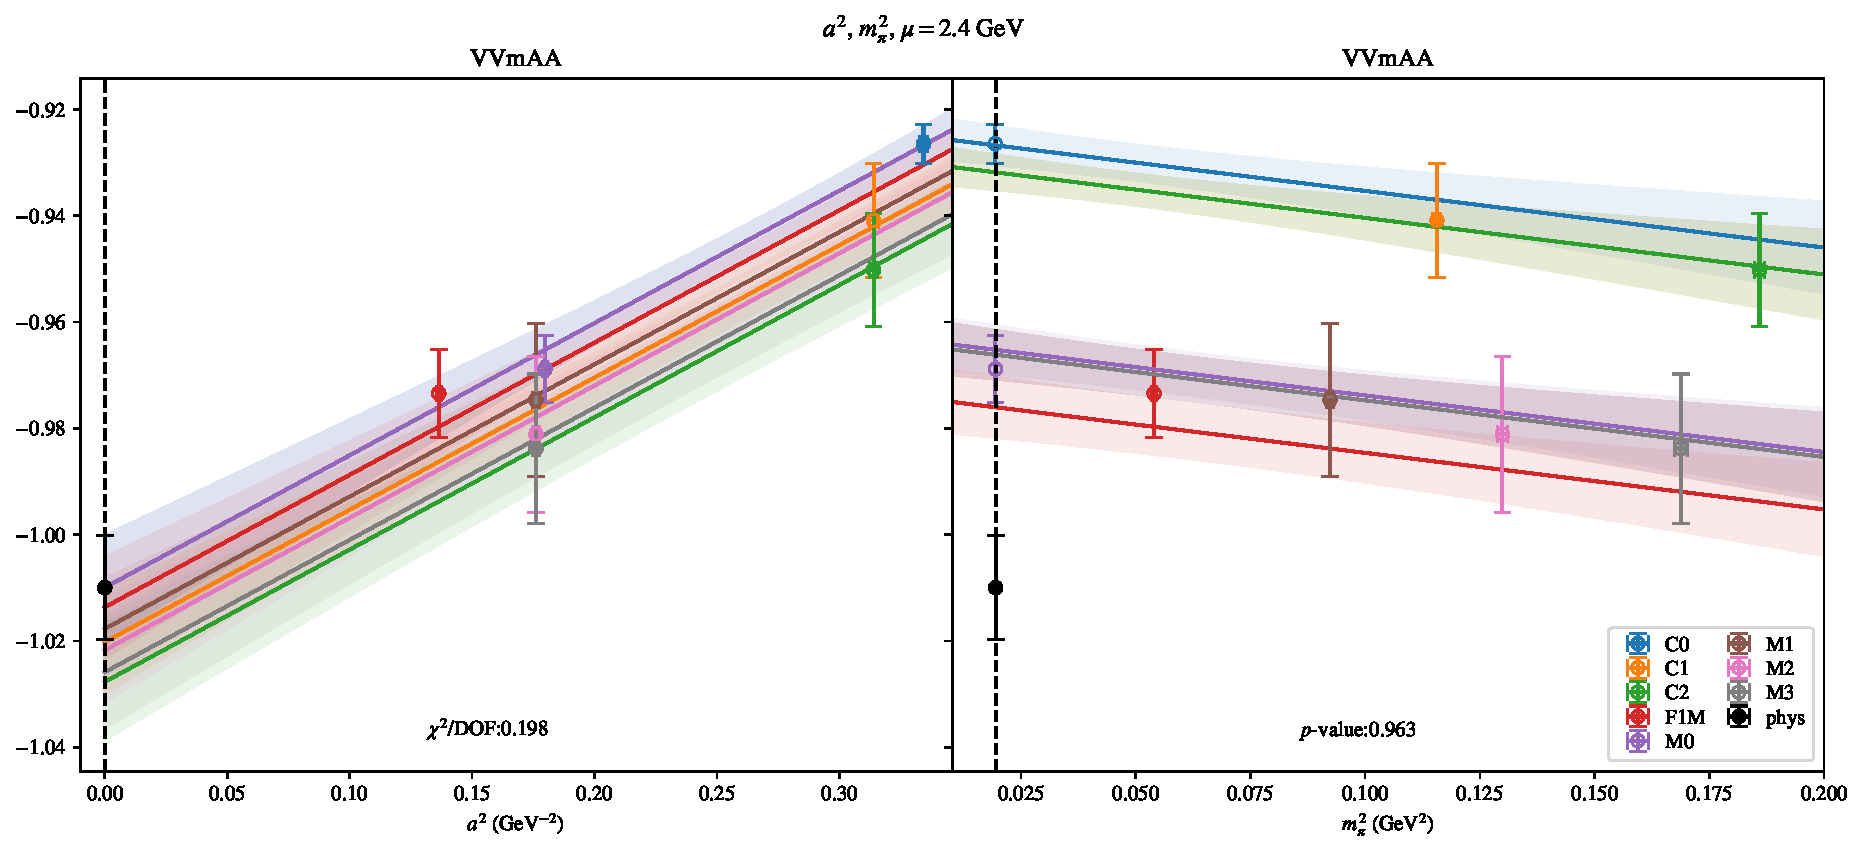
\includepdf[link, pages=-]{VVmAA/NPR/bag_a2m2_24.pdf}
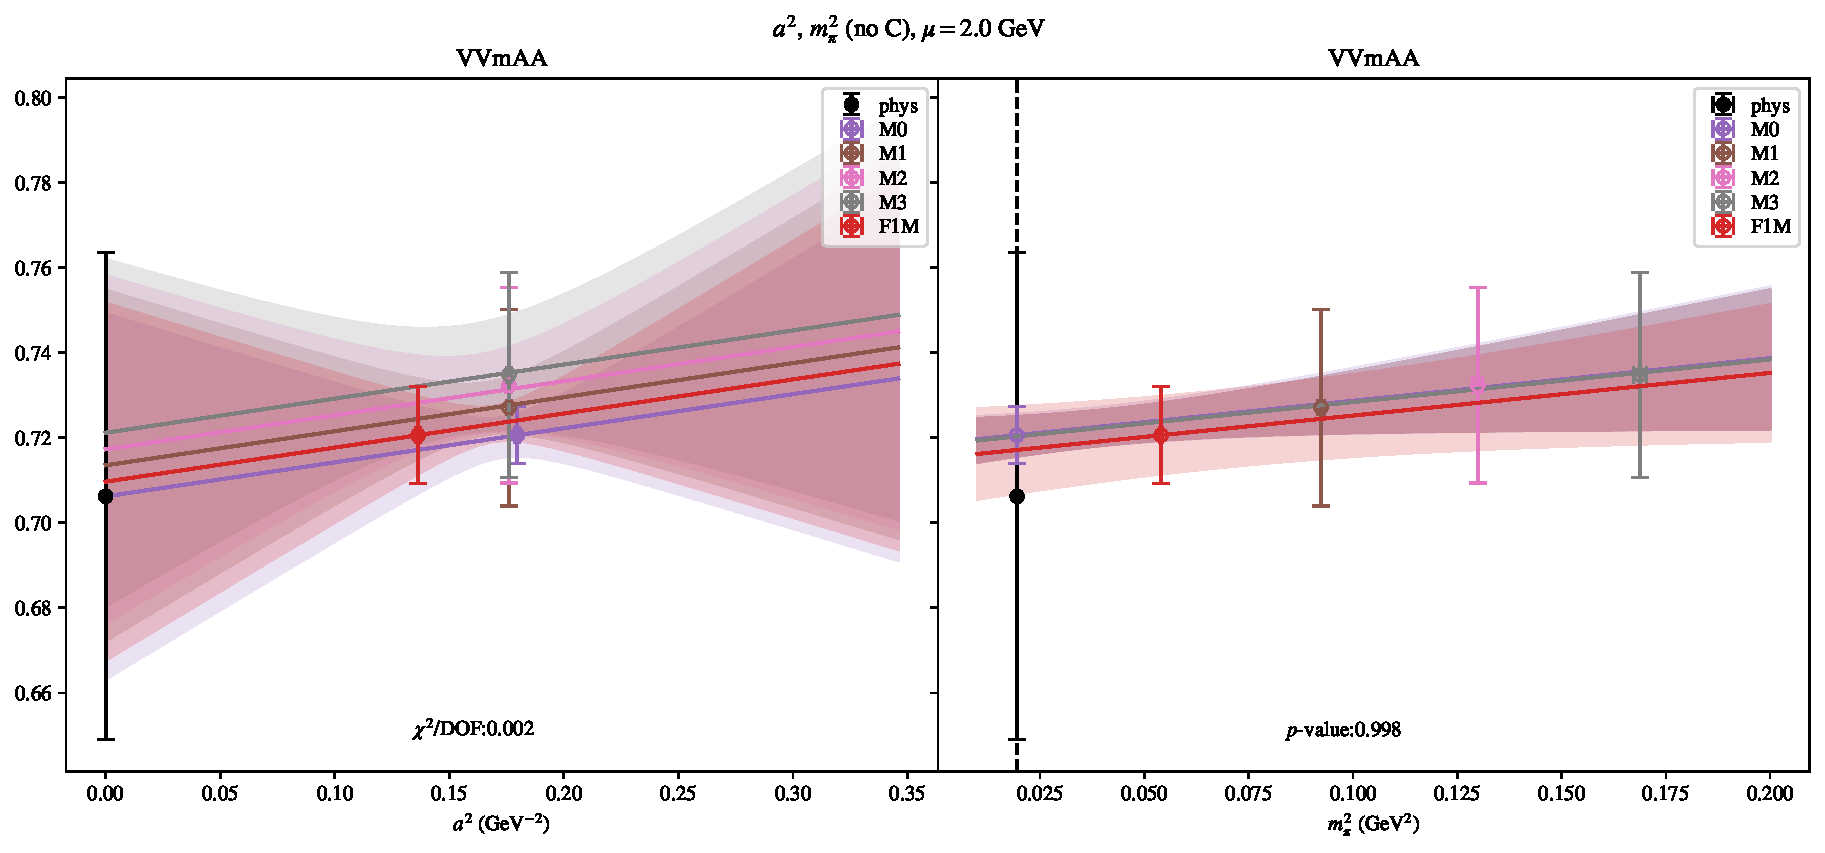
\includepdf[link, pages=-]{VVmAA/NPR/bag_a2m2noC_20.pdf}
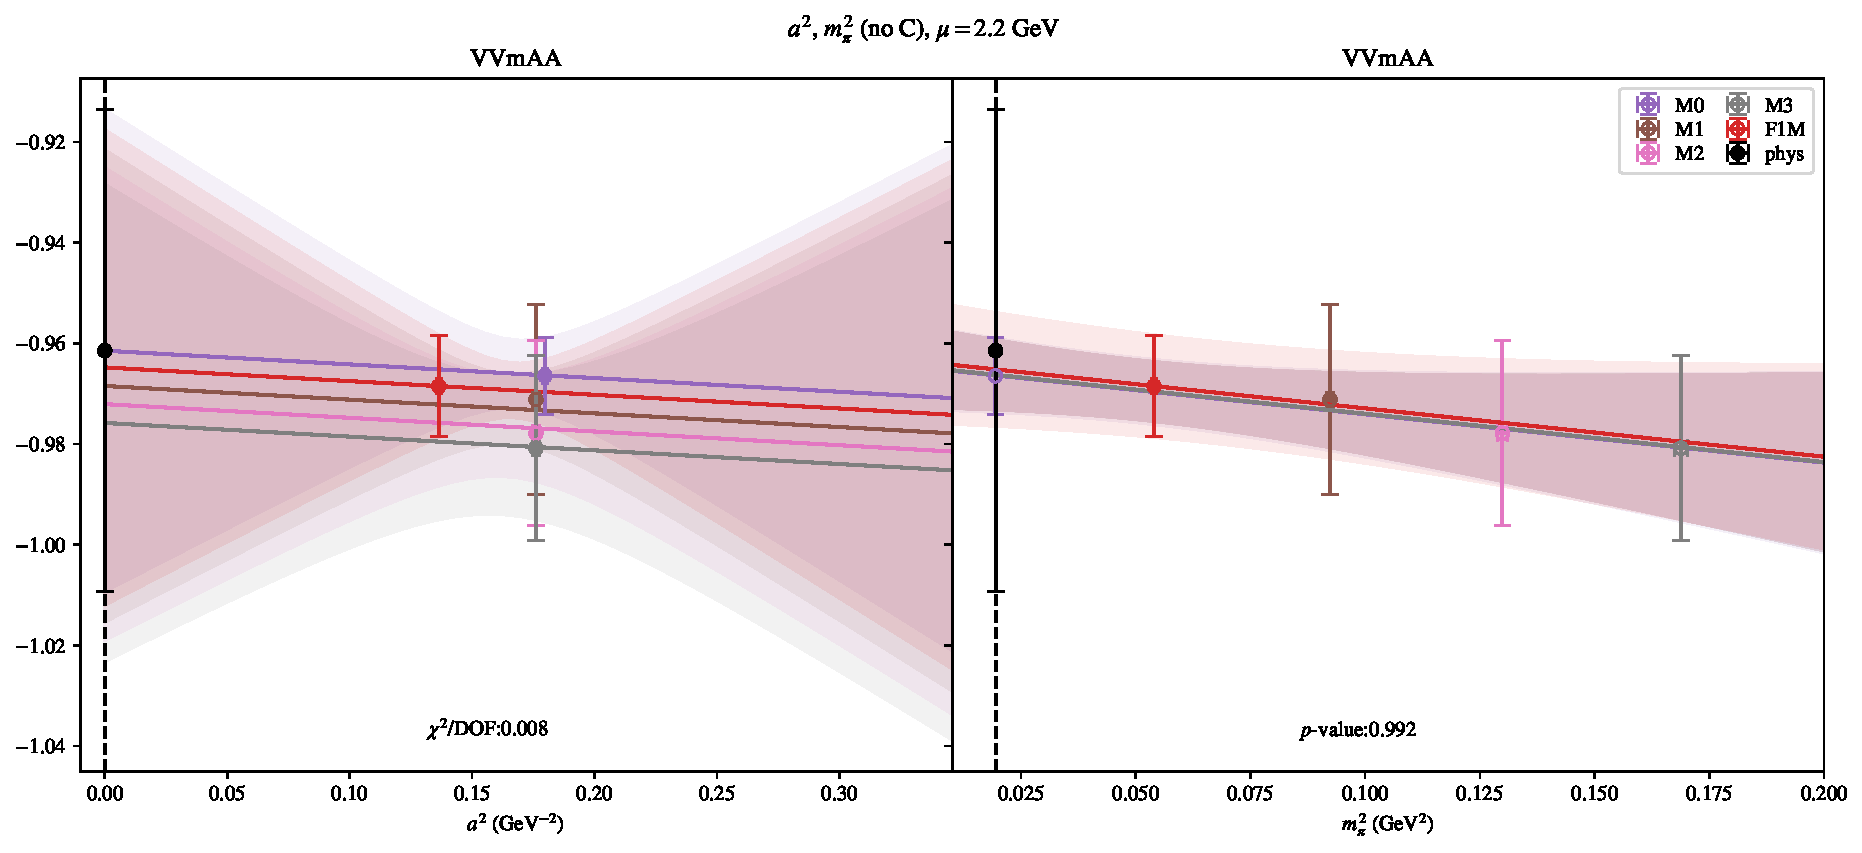
\includepdf[link, pages=-]{VVmAA/NPR/bag_a2m2noC_22.pdf}
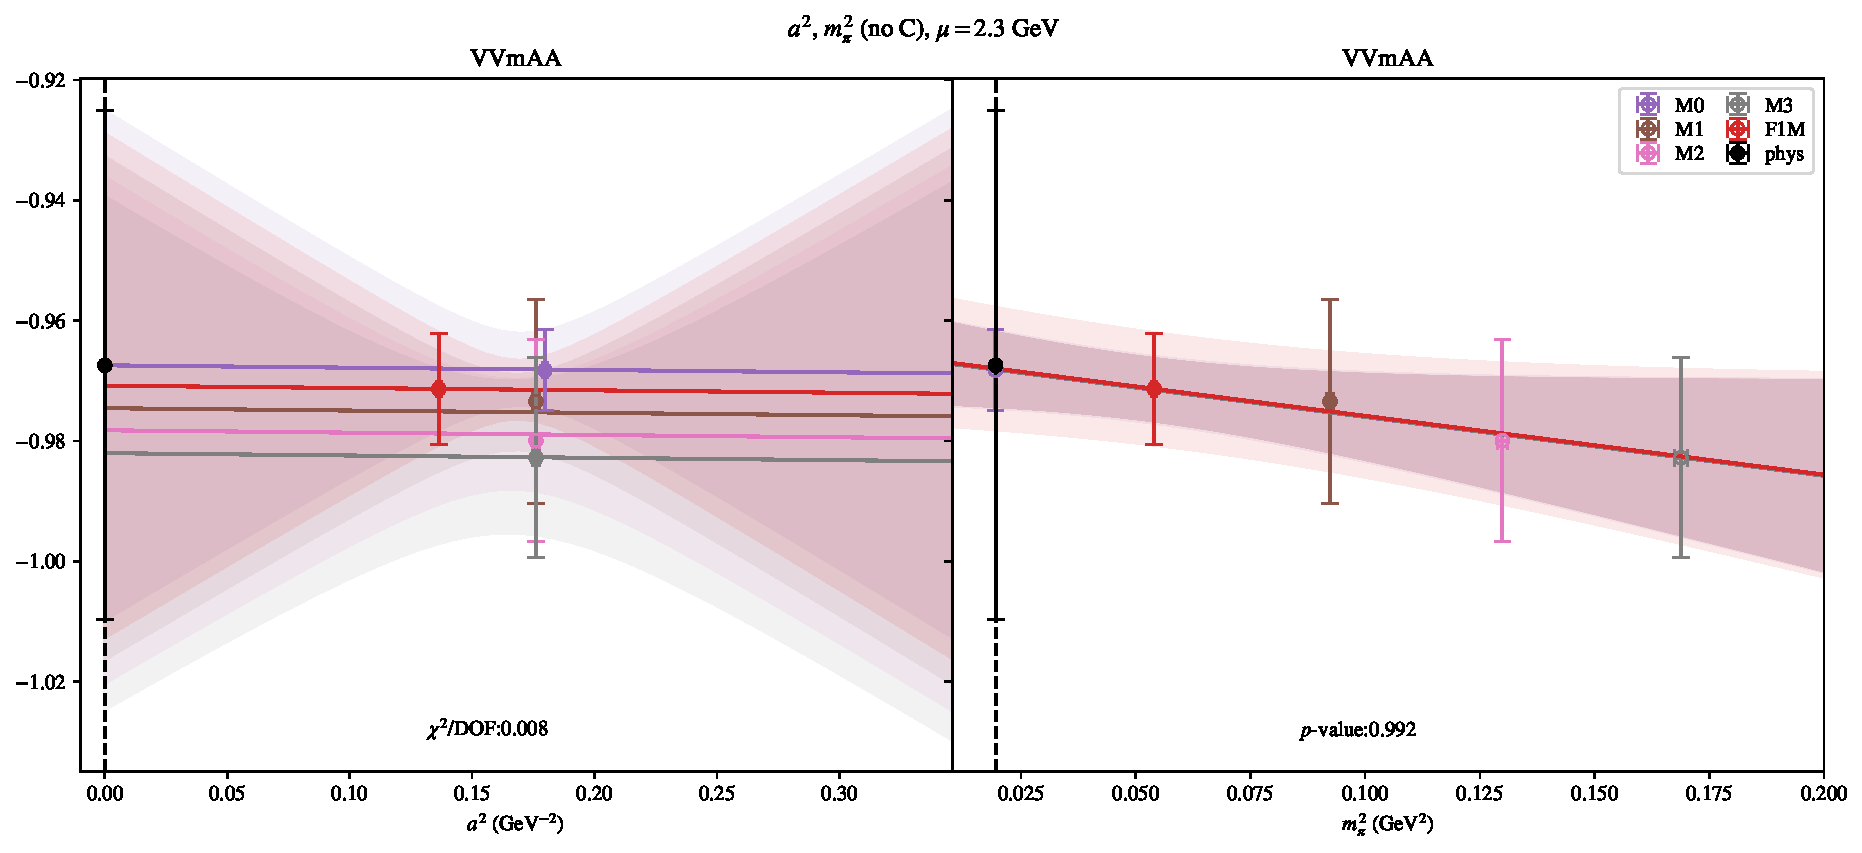
\includepdf[link, pages=-]{VVmAA/NPR/bag_a2m2noC_23.pdf}
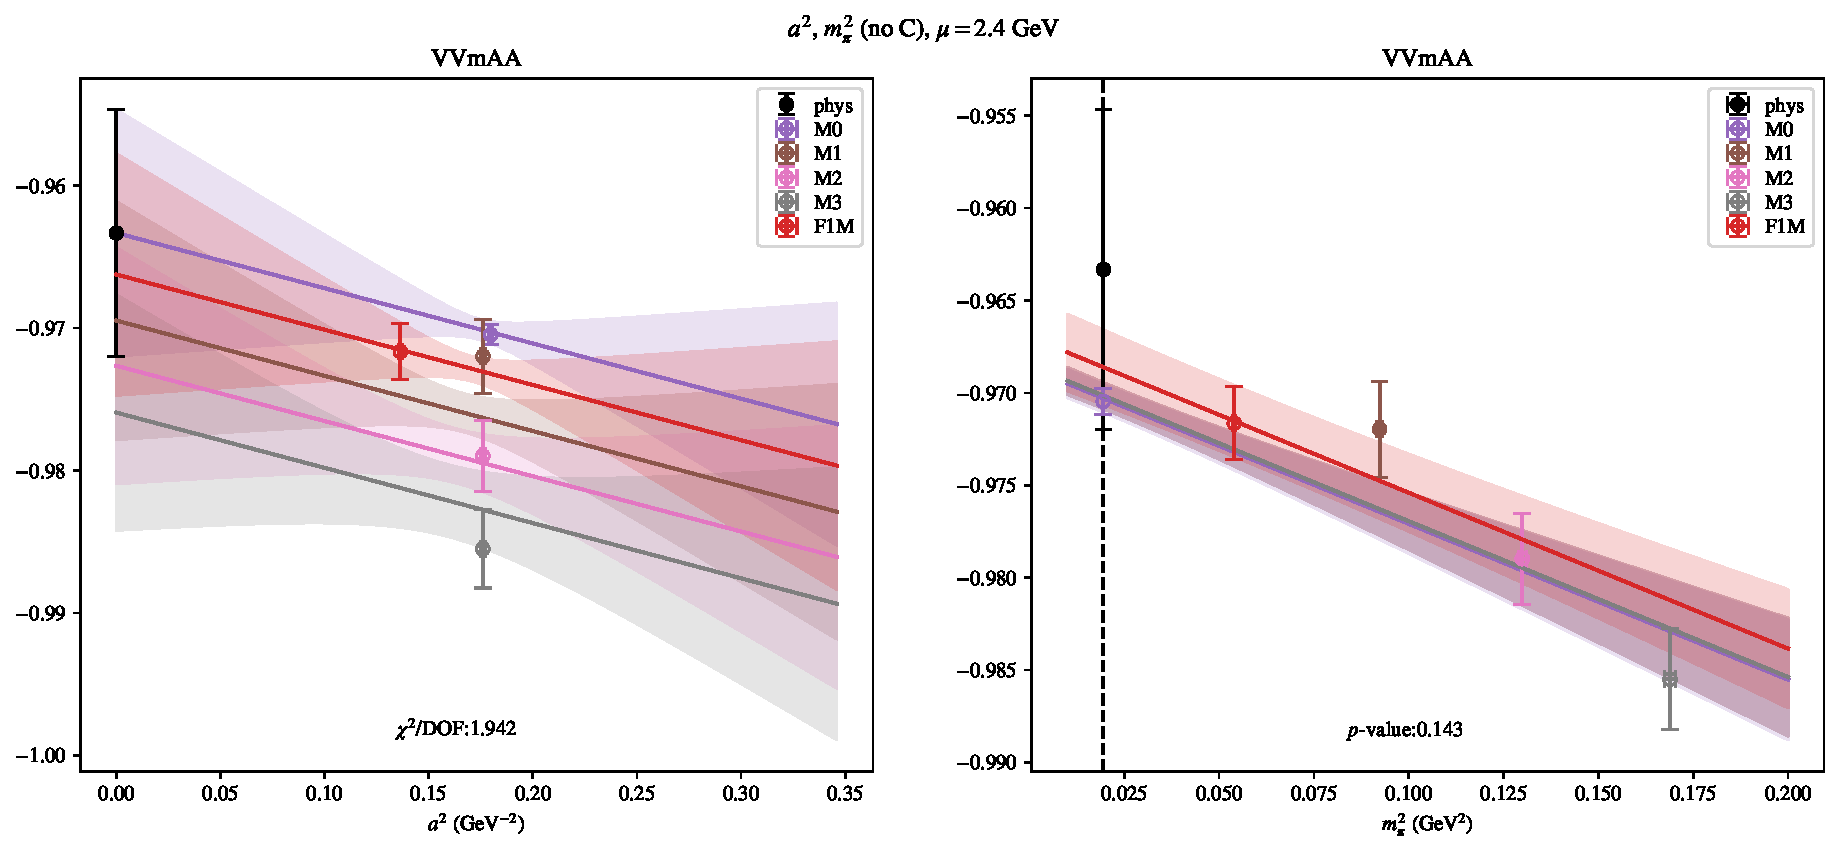
\includepdf[link, pages=-]{VVmAA/NPR/bag_a2m2noC_24.pdf}
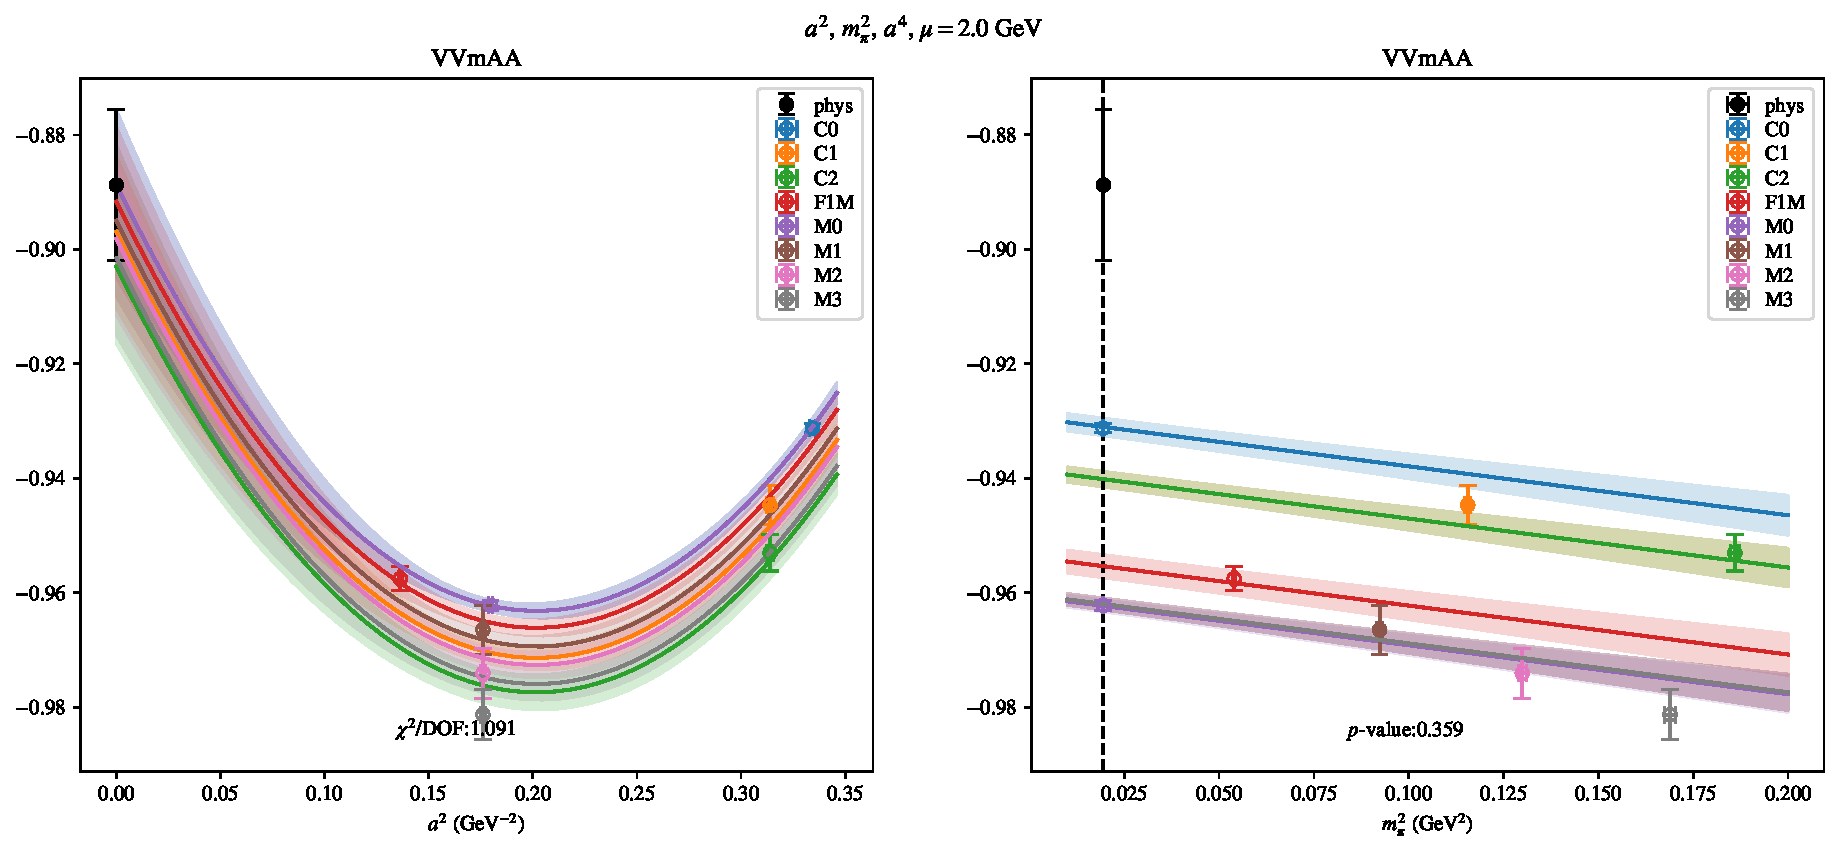
\includepdf[link, pages=-]{VVmAA/NPR/bag_a2a4m2_20.pdf}
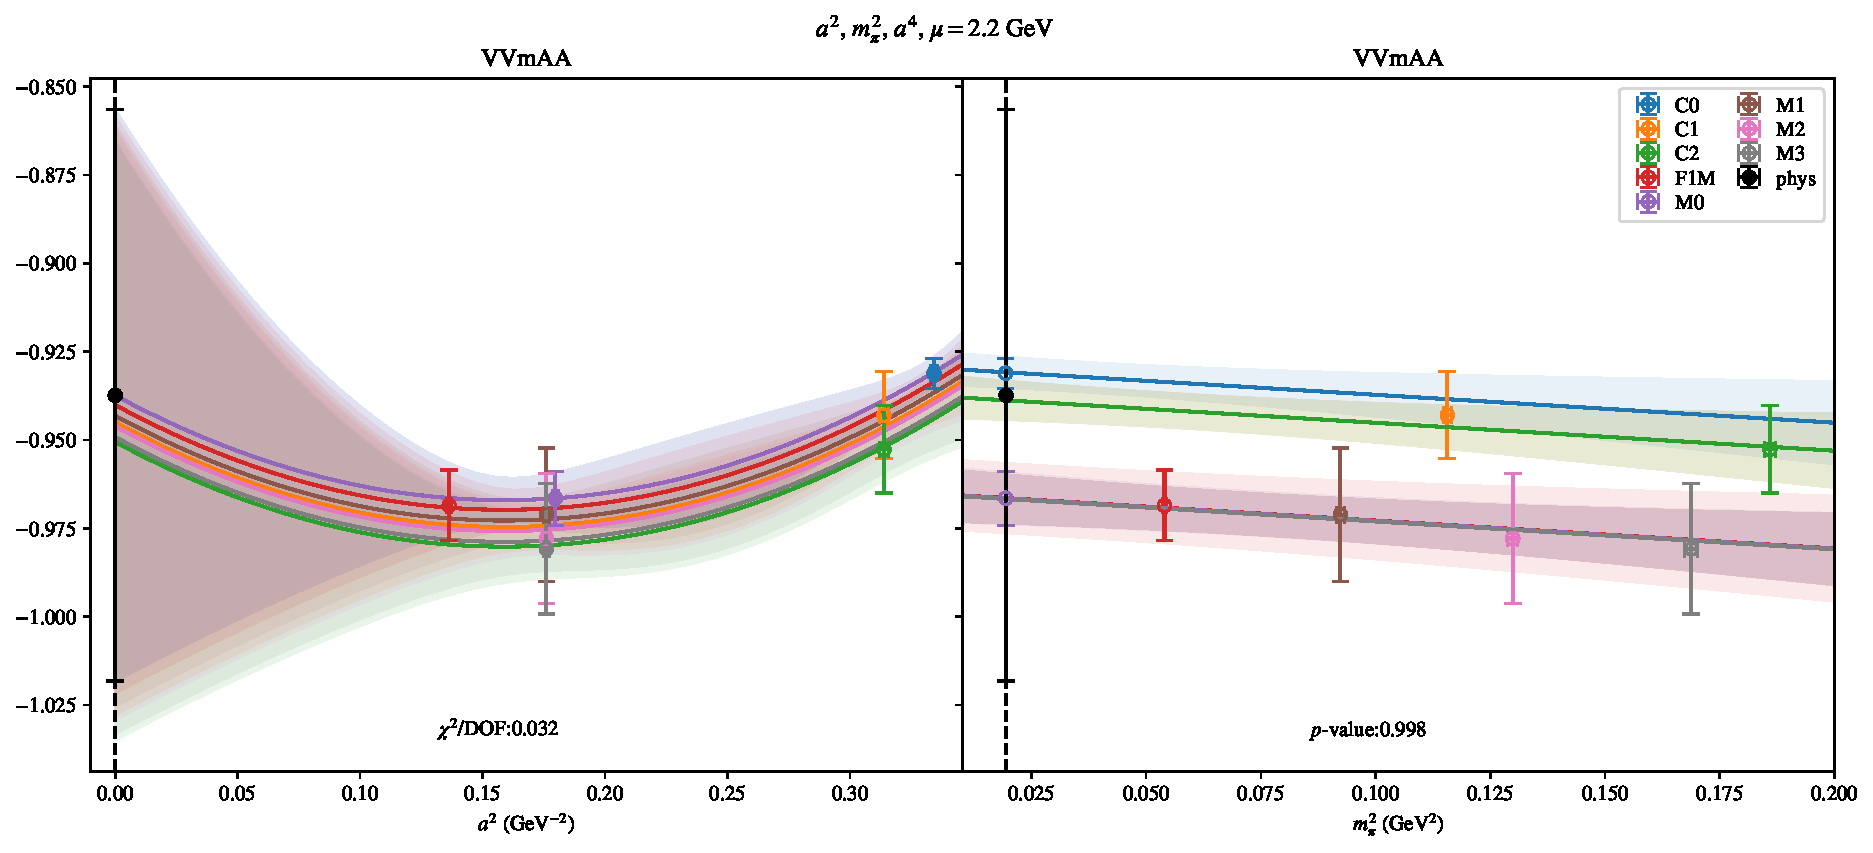
\includepdf[link, pages=-]{VVmAA/NPR/bag_a2a4m2_22.pdf}
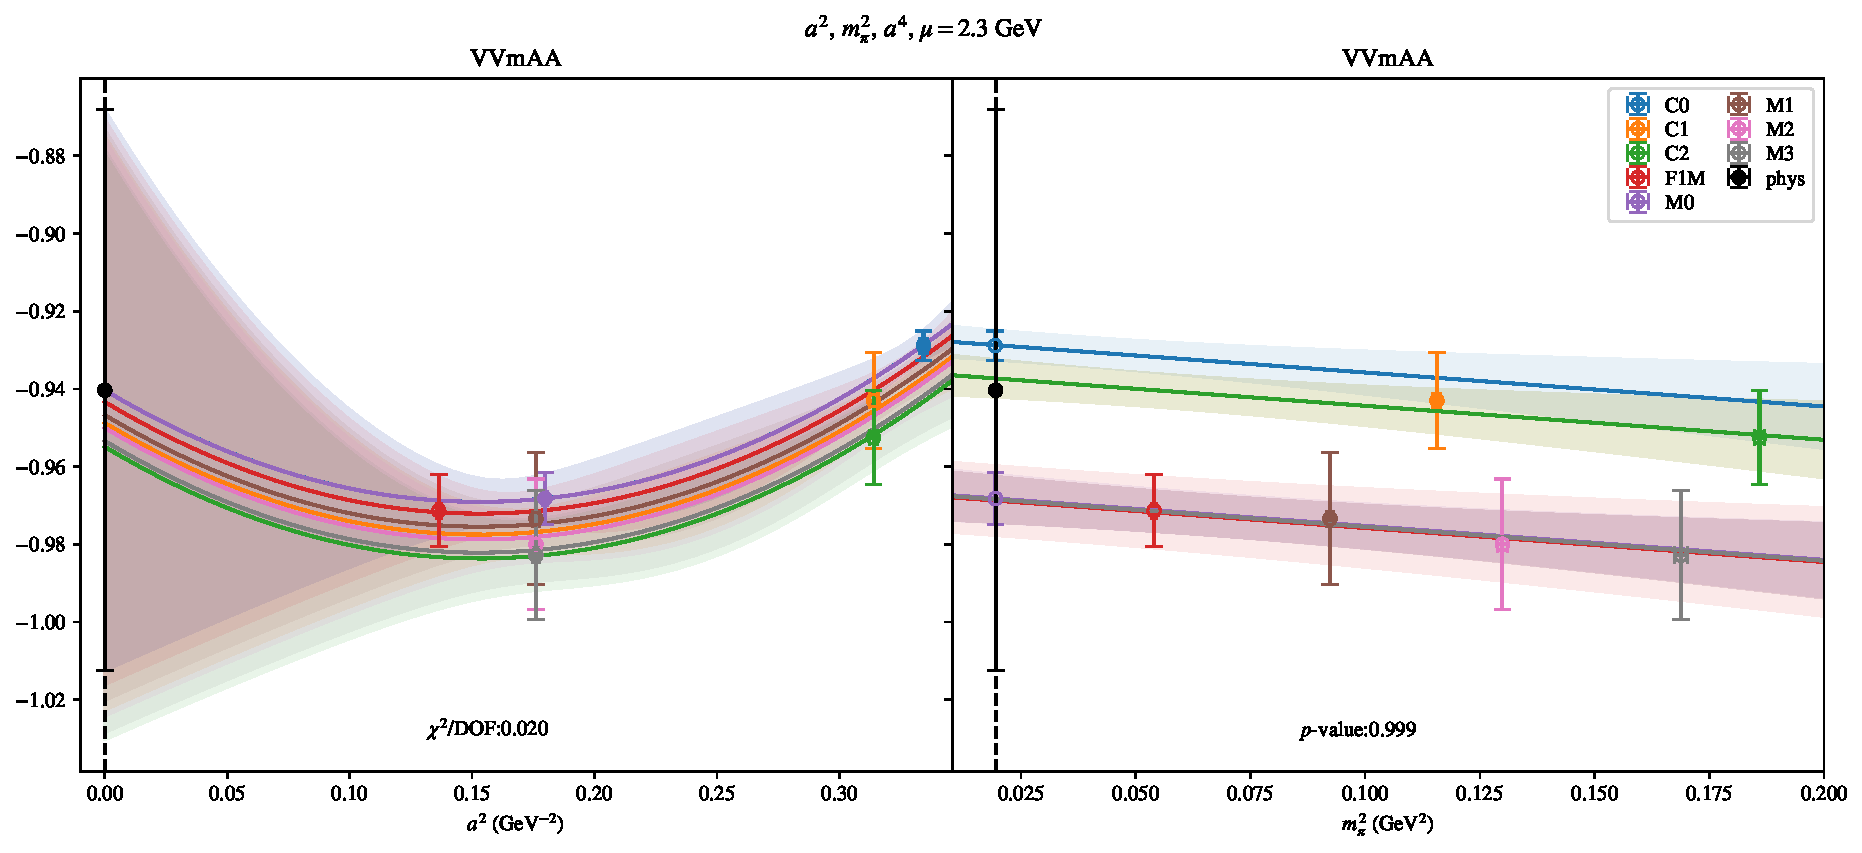
\includepdf[link, pages=-]{VVmAA/NPR/bag_a2a4m2_23.pdf}
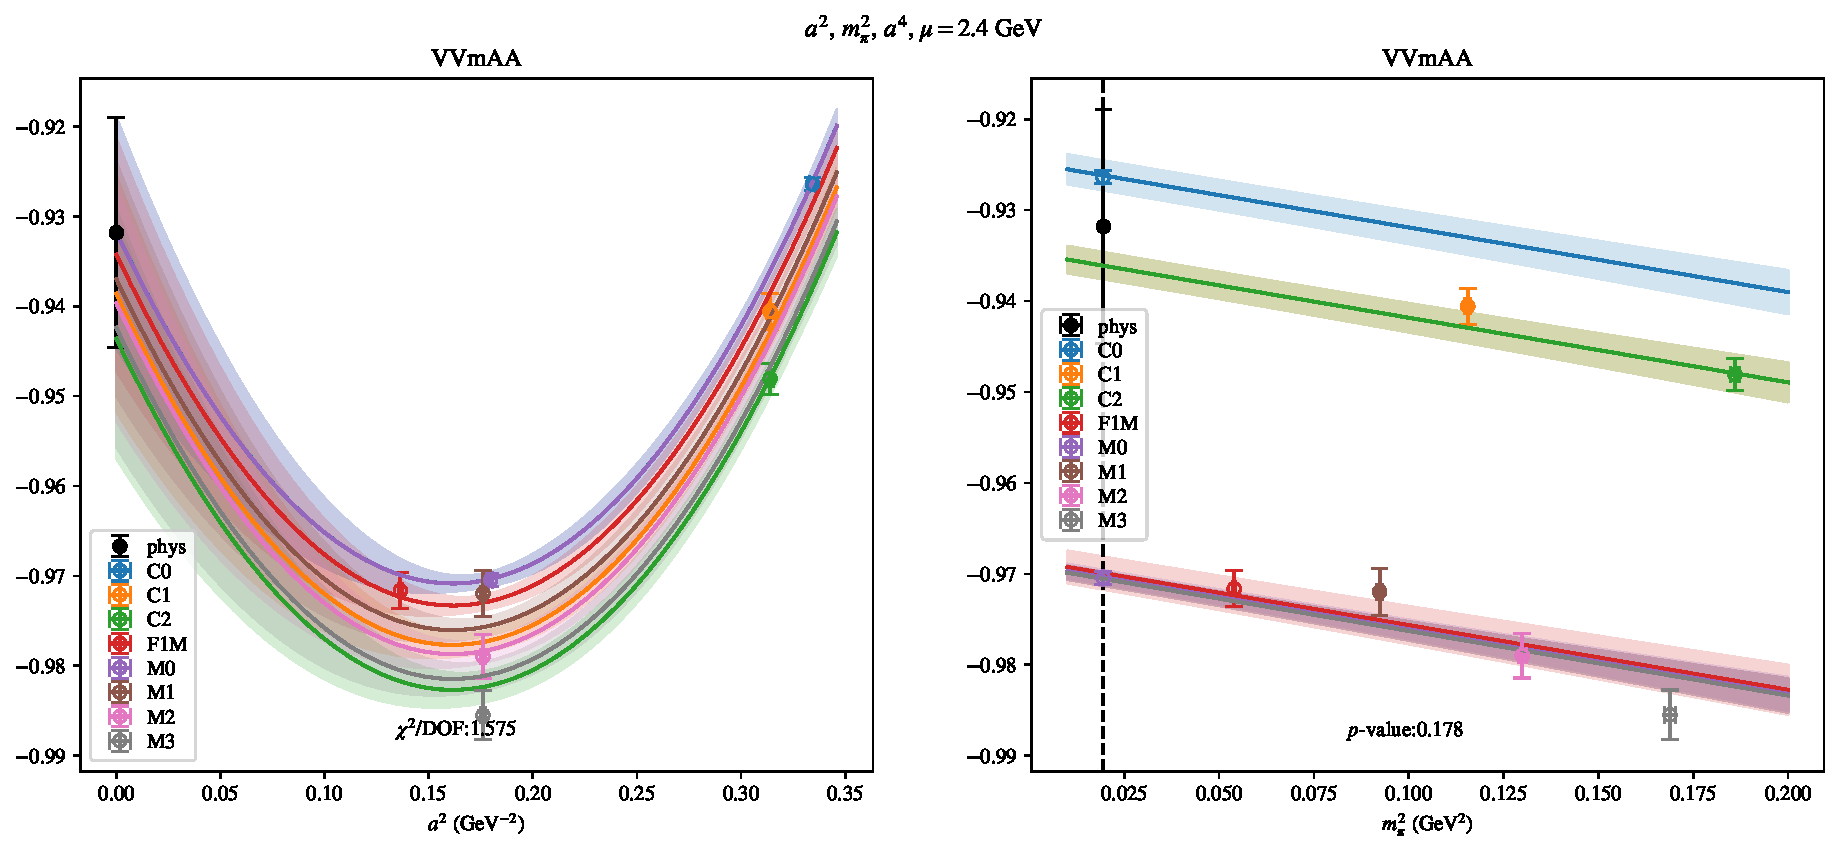
\includepdf[link, pages=-]{VVmAA/NPR/bag_a2a4m2_24.pdf}
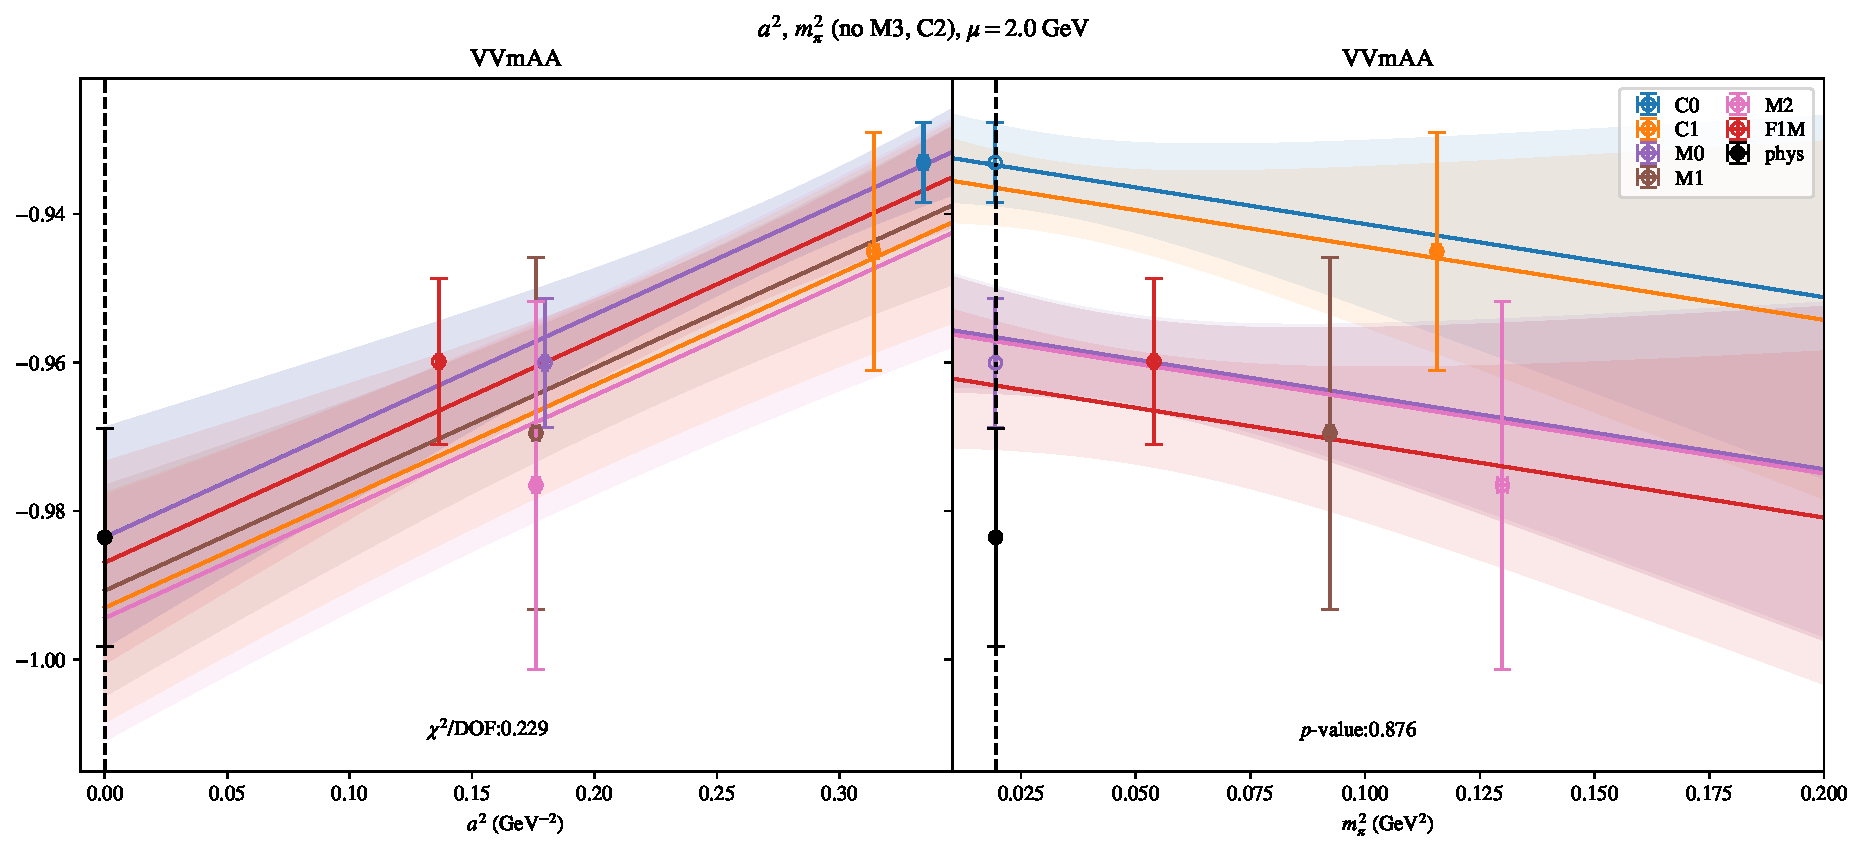
\includepdf[link, pages=-]{VVmAA/NPR/bag_a2m2mcut_20.pdf}
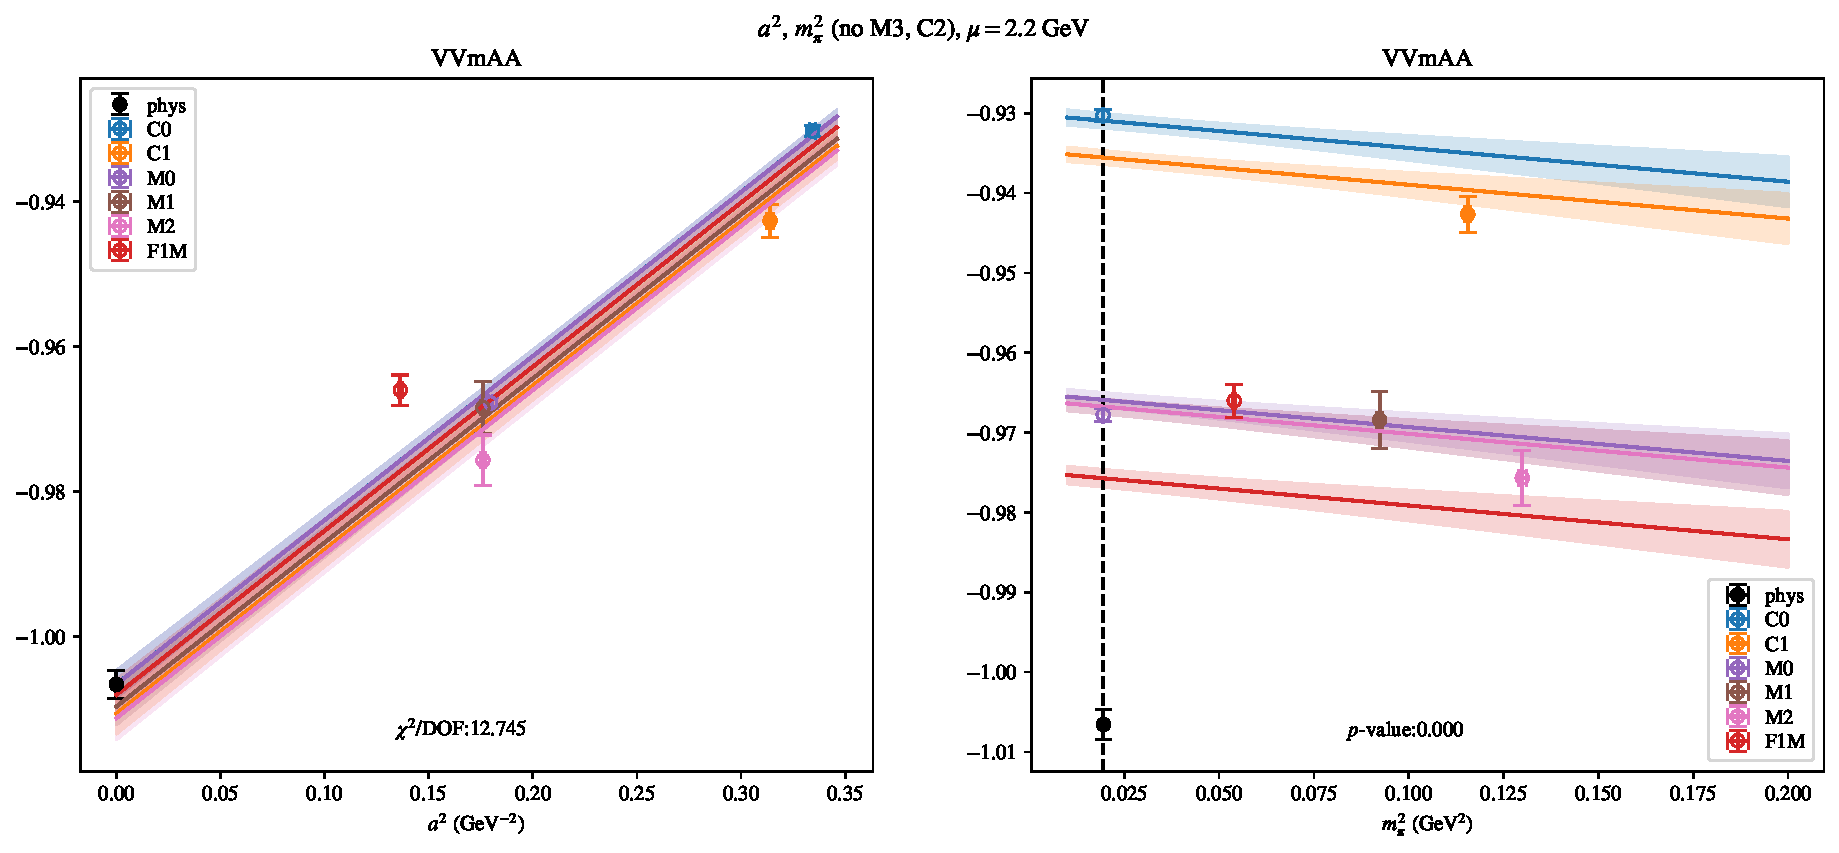
\includepdf[link, pages=-]{VVmAA/NPR/bag_a2m2mcut_22.pdf}
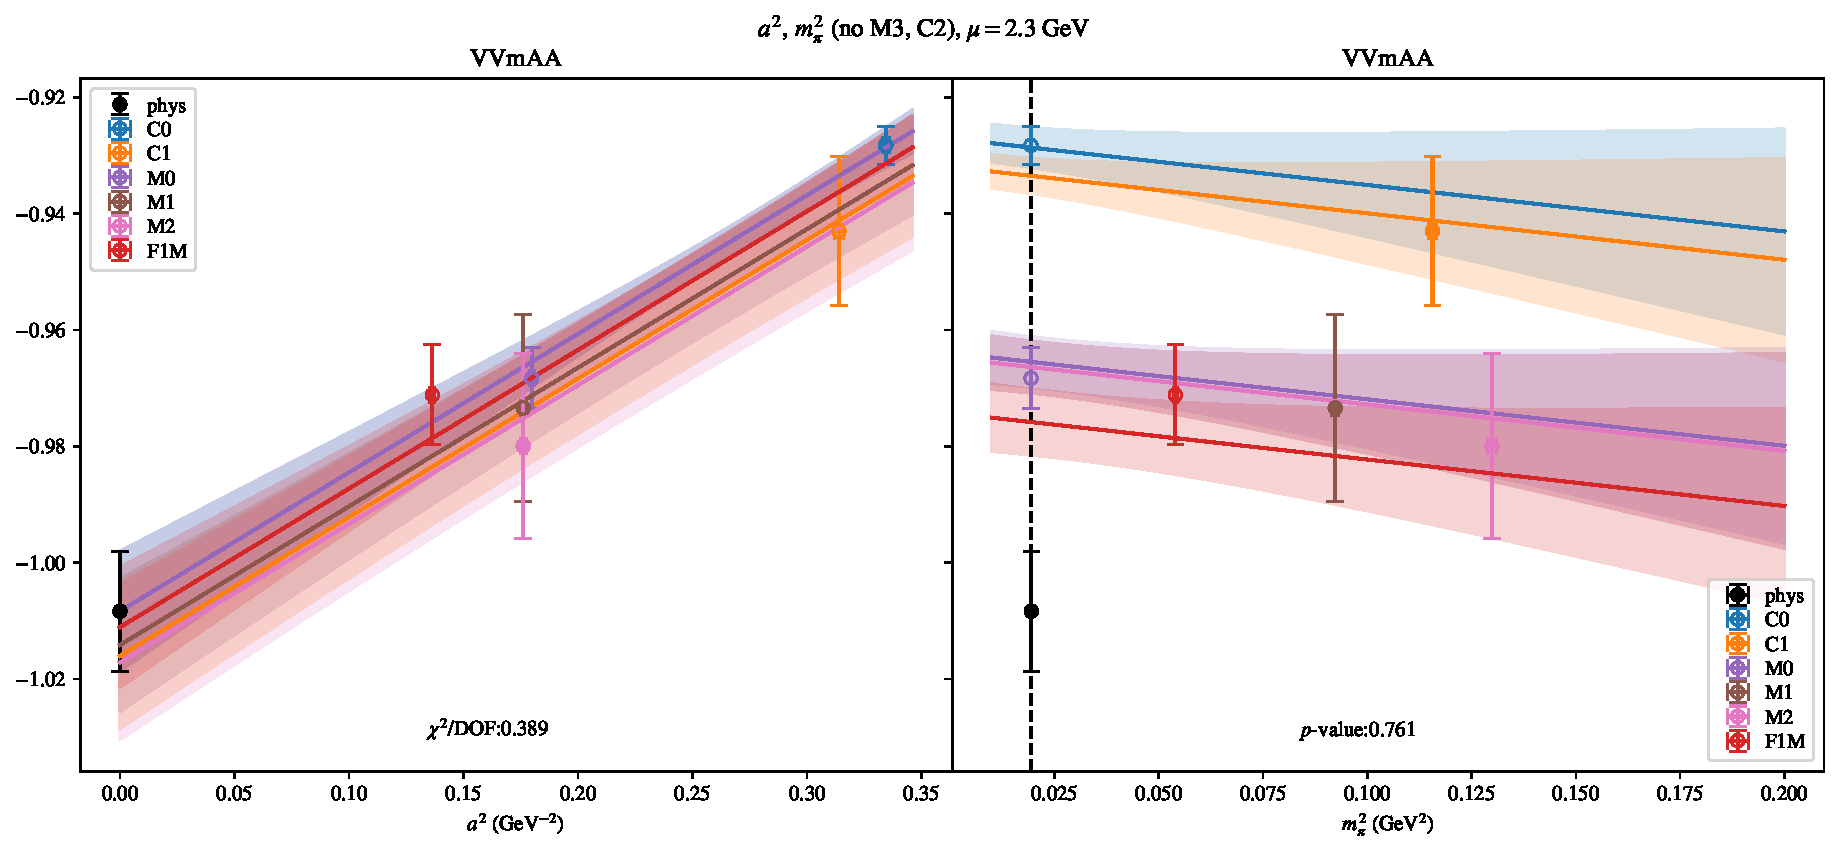
\includepdf[link, pages=-]{VVmAA/NPR/bag_a2m2mcut_23.pdf}
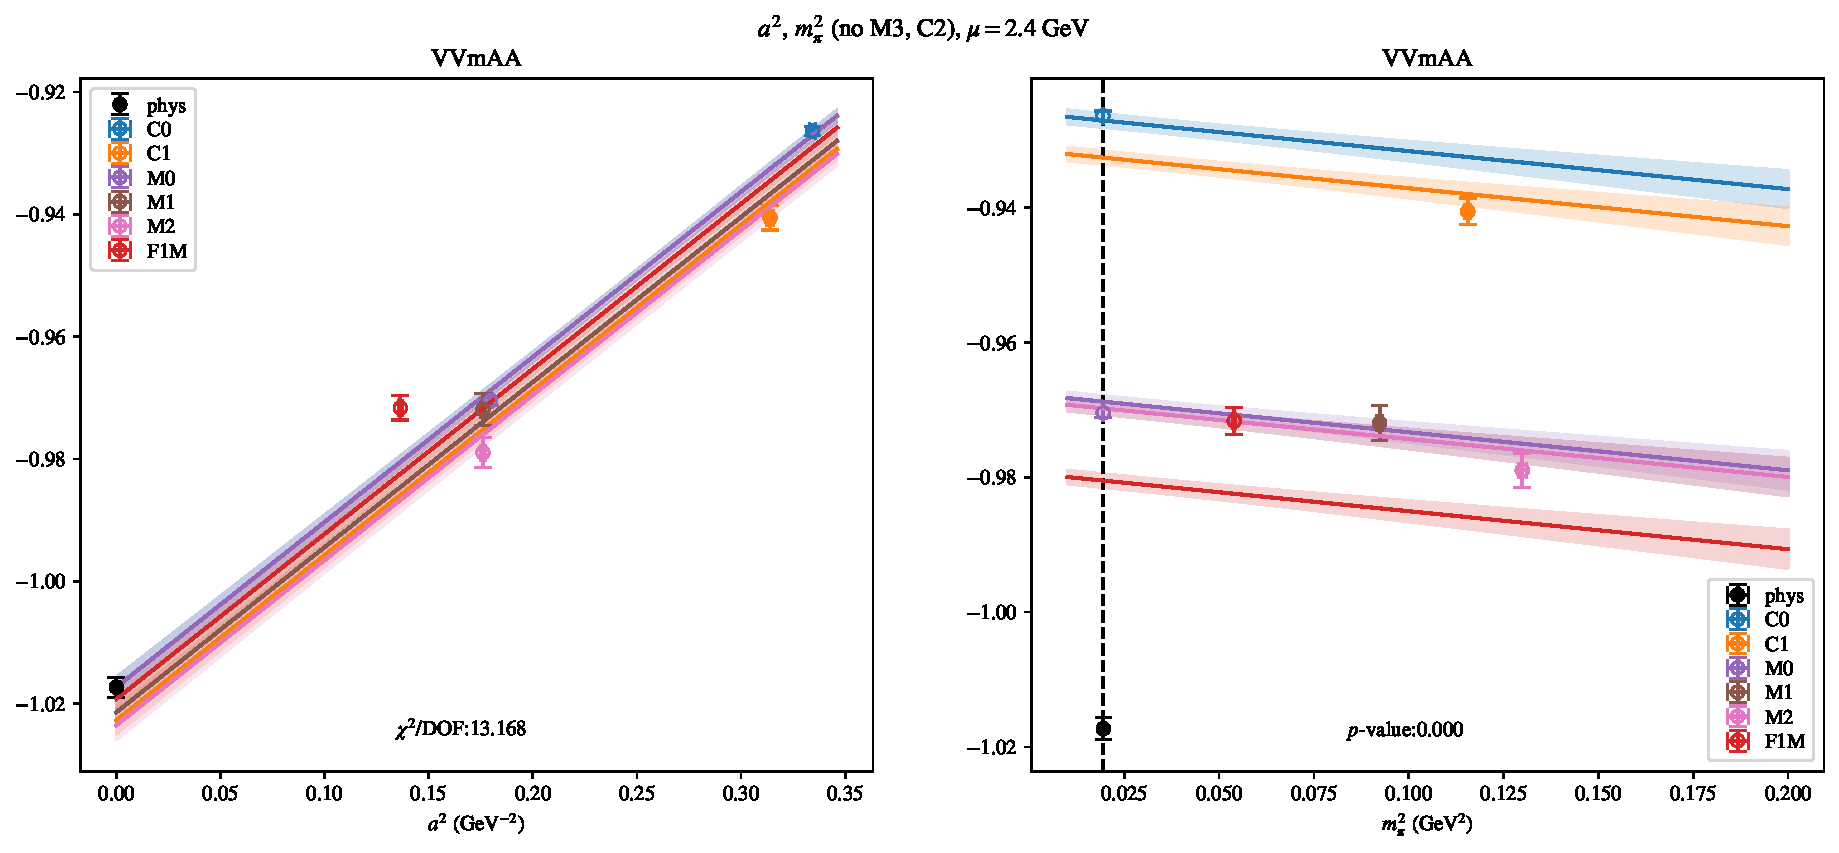
\includepdf[link, pages=-]{VVmAA/NPR/bag_a2m2mcut_24.pdf}
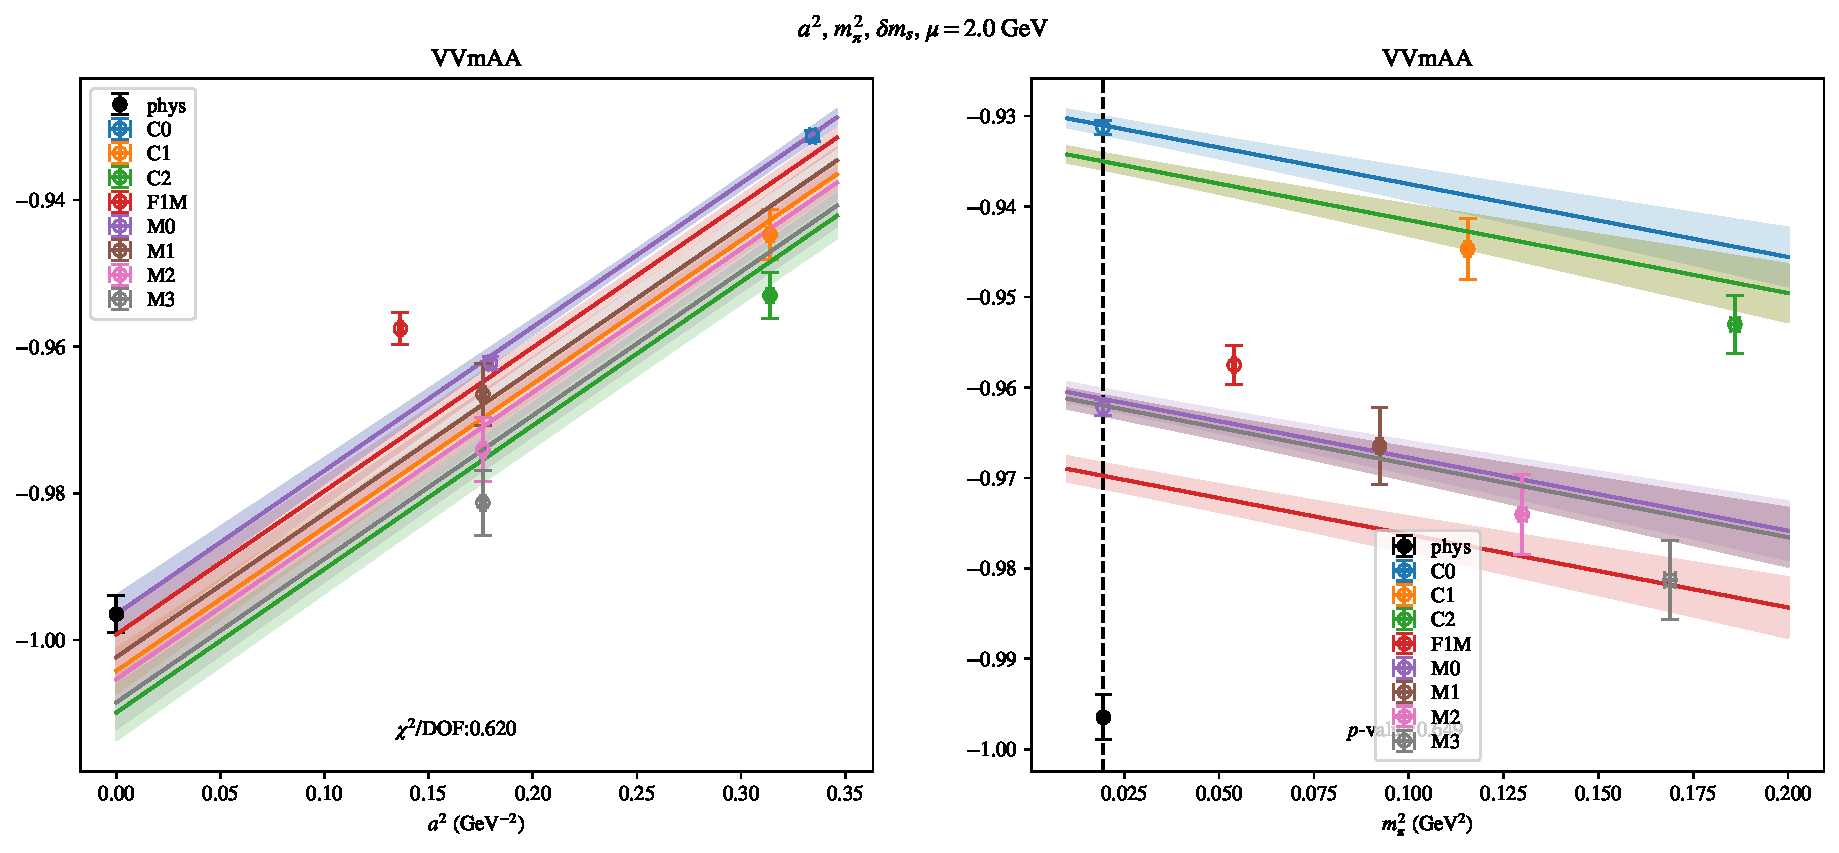
\includepdf[link, pages=-]{VVmAA/NPR/bag_a2m2delm_20.pdf}
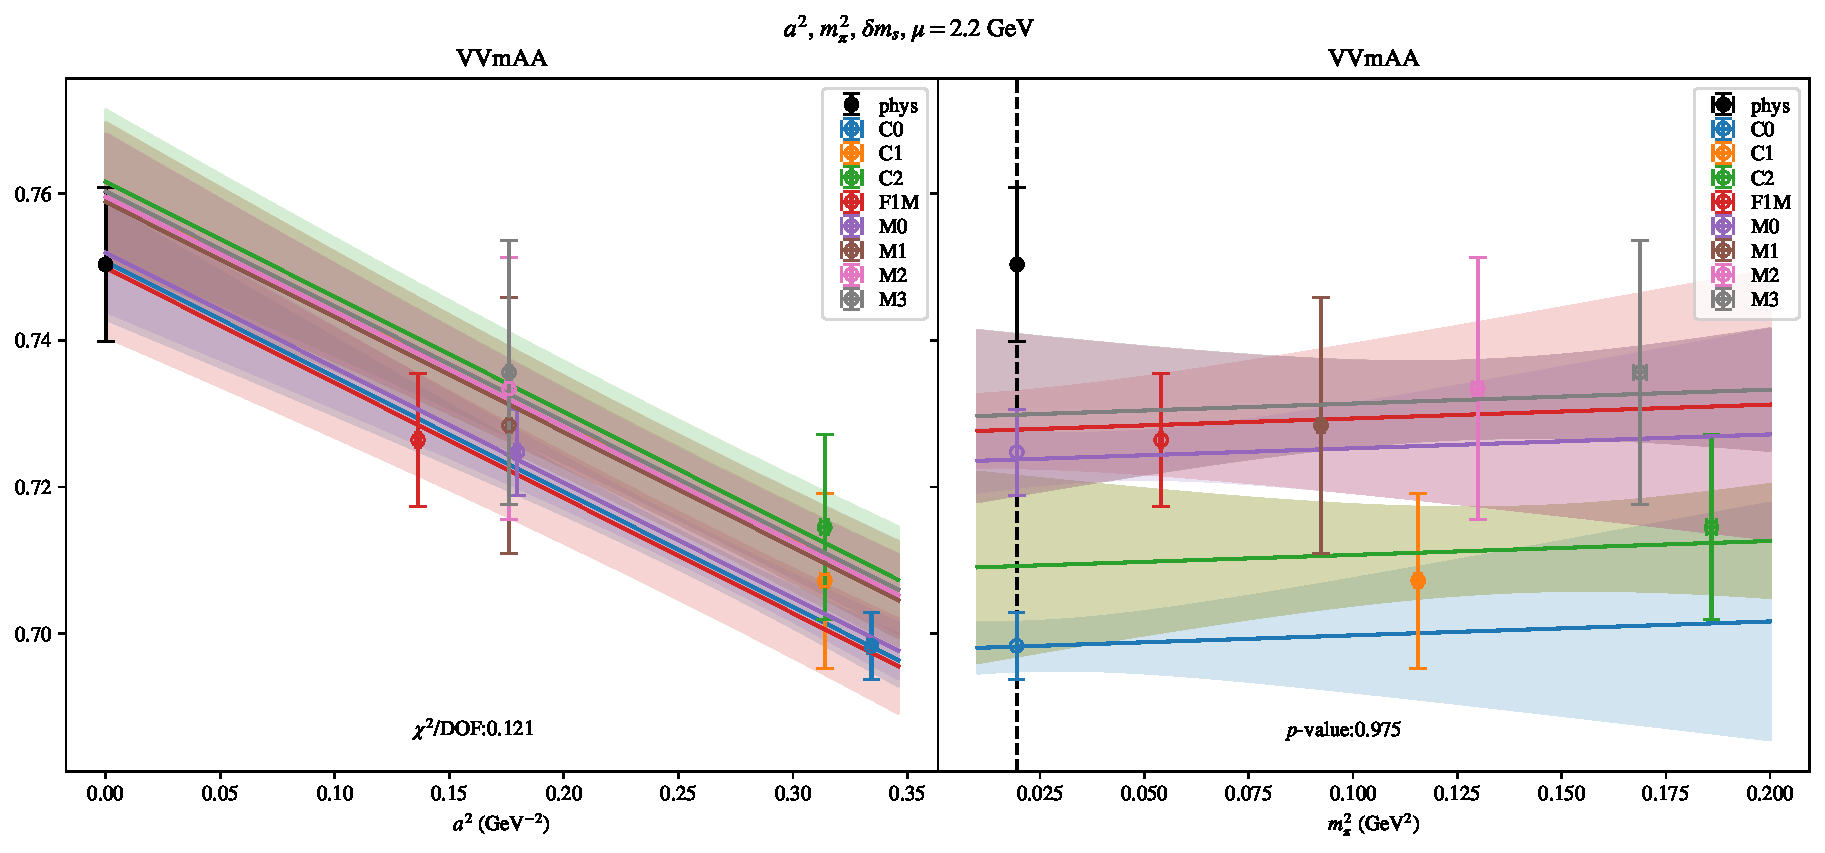
\includepdf[link, pages=-]{VVmAA/NPR/bag_a2m2delm_22.pdf}
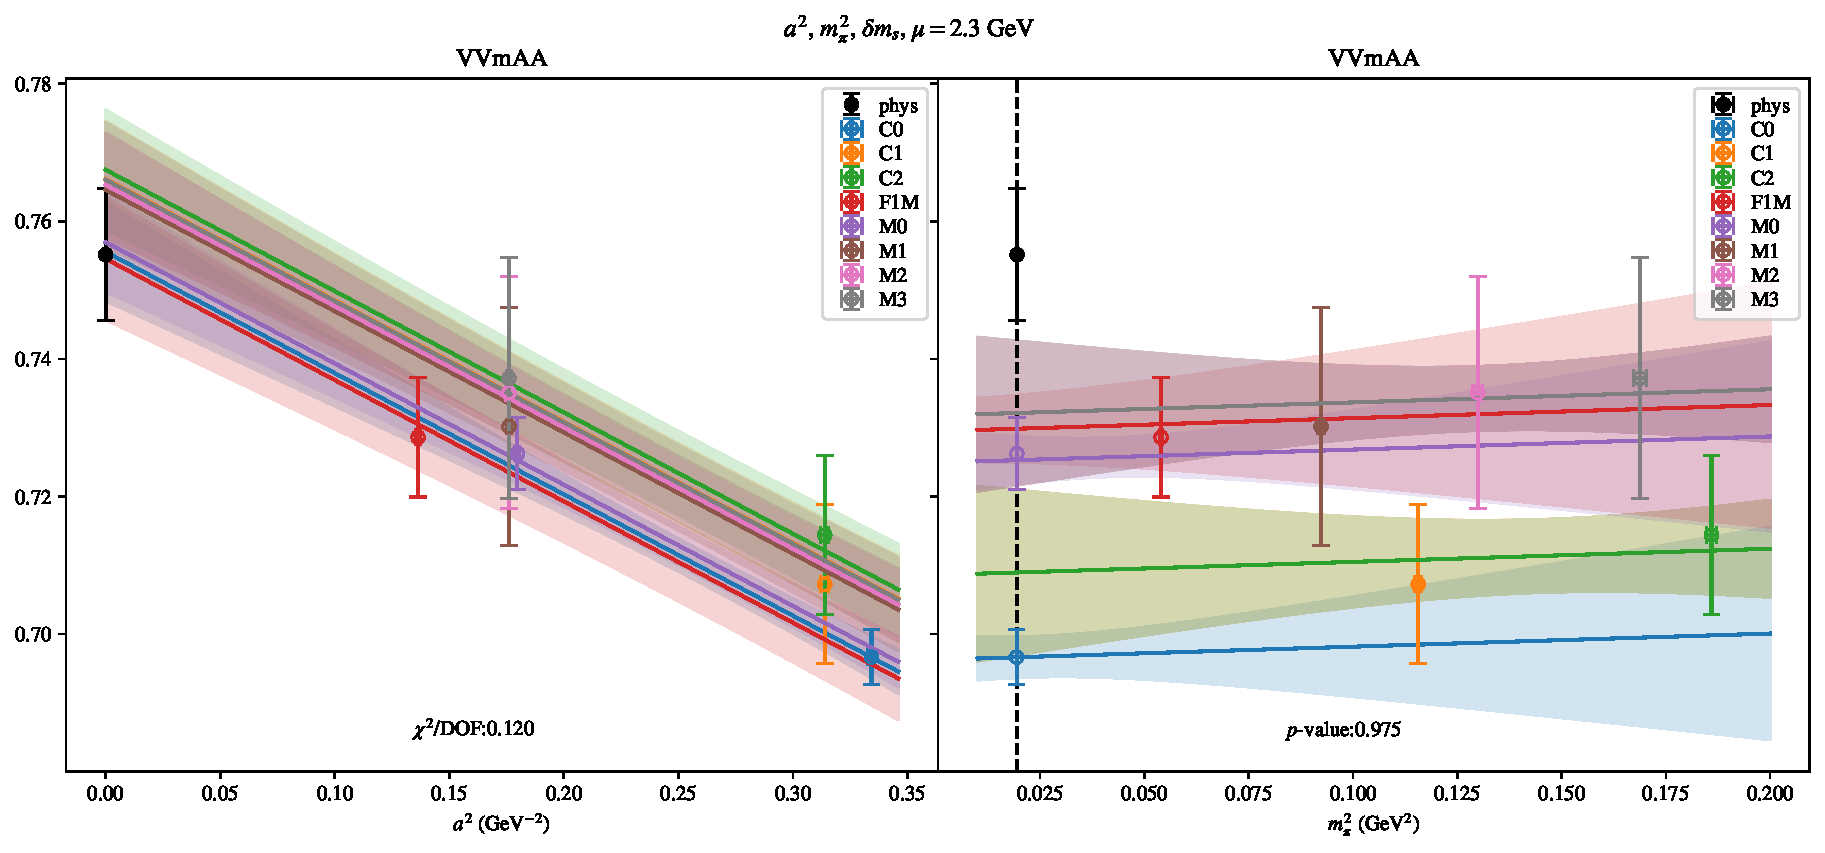
\includepdf[link, pages=-]{VVmAA/NPR/bag_a2m2delm_23.pdf}
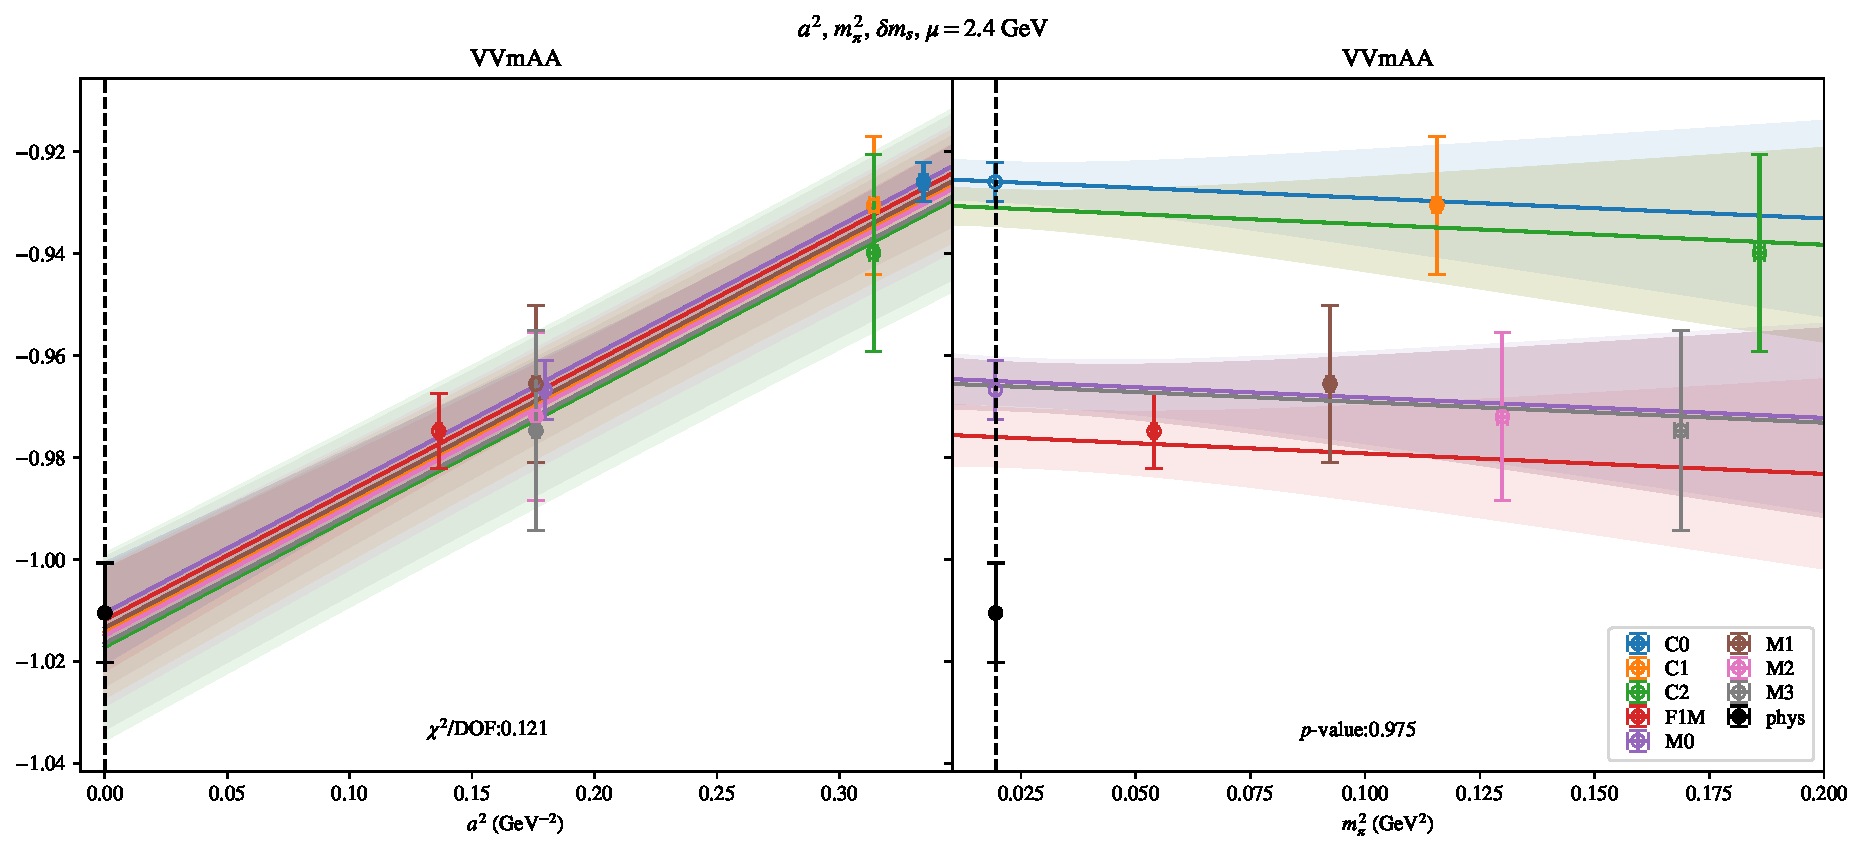
\includepdf[link, pages=-]{VVmAA/NPR/bag_a2m2delm_24.pdf}
\clearpage
\section{$\mathcal{B}_3$}
\begin{table}[h!]
\begin{center}
\begin{tabular}{|c|c|c|c|c|c|}
\hline
$\mu$ (GeV) & $a^2$, $m_\pi^2$& $a^2$, $m_\pi^2$ (no C)& $a^2$, $m_\pi^2$, $a^4$& $a^2$, $m_\pi^2$ (no M3, C2)& $a^2$, $m_\pi^2$, $\delta m_s$\\
\hline
2.0& \hyperlink{SSmPP/NPR/bag_a2m2_20.pdf.1}{\textbf{1.7969(43)}: 5.733 (0.0)} & \hyperlink{SSmPP/NPR/bag_a2m2noC_20.pdf.1}{\textbf{1.703(20)}: 0.051 (0.95)} & \hyperlink{SSmPP/NPR/bag_a2a4m2_20.pdf.1}{\textbf{1.650(32)}: 0.864 (0.485)} & \hyperlink{SSmPP/NPR/bag_a2m2mcut_20.pdf.1}{\textbf{1.7966(48)}: 9.229 (0.0)} & \hyperlink{SSmPP/NPR/bag_a2m2delm_20.pdf.1}{\textbf{1.7963(59)}: 2.483 (0.042)}\\
2.2& \hyperlink{SSmPP/NPR/bag_a2m2_22.pdf.1}{\textbf{1.8014(36)}: 6.954 (0.0)} & \hyperlink{SSmPP/NPR/bag_a2m2noC_22.pdf.1}{\textbf{1.717(18)}: 0.153 (0.858)} & \hyperlink{SSmPP/NPR/bag_a2a4m2_22.pdf.1}{\textbf{1.666(27)}: 0.966 (0.425)} & \hyperlink{SSmPP/NPR/bag_a2m2mcut_22.pdf.1}{\textbf{1.8027(40)}: 10.629 (0.0)} & \hyperlink{SSmPP/NPR/bag_a2m2delm_22.pdf.1}{\textbf{1.8017(49)}: 3.918 (0.003)}\\
2.3& \hyperlink{SSmPP/NPR/bag_a2m2_23.pdf.1}{\textbf{1.8034(34)}: 7.201 (0.0)} & \hyperlink{SSmPP/NPR/bag_a2m2noC_23.pdf.1}{\textbf{1.721(17)}: 0.195 (0.823)} & \hyperlink{SSmPP/NPR/bag_a2a4m2_23.pdf.1}{\textbf{1.667(27)}: 0.722 (0.577)} & \hyperlink{SSmPP/NPR/bag_a2m2mcut_23.pdf.1}{\textbf{1.8044(38)}: 11.696 (0.0)} & \hyperlink{SSmPP/NPR/bag_a2m2delm_23.pdf.1}{\textbf{1.8033(47)}: 4.047 (0.003)}\\
2.4& \hyperlink{SSmPP/NPR/bag_a2m2_24.pdf.1}{\textbf{1.8055(34)}: 6.765 (0.0)} & \hyperlink{SSmPP/NPR/bag_a2m2noC_24.pdf.1}{\textbf{1.726(17)}: 0.219 (0.803)} & \hyperlink{SSmPP/NPR/bag_a2a4m2_24.pdf.1}{\textbf{1.675(26)}: 0.823 (0.51)} & \hyperlink{SSmPP/NPR/bag_a2m2mcut_24.pdf.1}{\textbf{1.8062(38)}: 10.942 (0.0)} & \hyperlink{SSmPP/NPR/bag_a2m2delm_24.pdf.1}{\textbf{1.8052(44)}: 4.266 (0.002)}\\
\hline
\end{tabular}
\caption{Physical point value from chiral and continuum extrapolation at renormalisation scale $\mu$. Entries are \textbf{value(error)}: $\chi^2/\text{DOF}$ ($p$-value).}
\end{center}
\end{table}
\begin{table}[h!]
\begin{center}
\begin{tabular}{|c c|c|c|c|c|c|}
\hline
$\mu$ (GeV) &  & $a^2$, $m_\pi^2$& $a^2$, $m_\pi^2$ (no C)& $a^2$, $m_\pi^2$, $a^4$& $a^2$, $m_\pi^2$ (no M3, C2)& $a^2$, $m_\pi^2$, $\delta m_s$\\
\hline
\multirow{3}{0.5in}{2.0} & $\alpha$ & 0.146(17)& 0.70(11)& 1.48(28)& 0.148(19)& 0.137(22)\\
 & $\beta$ & -0.00062(46)& 0.00016(79)& -0.00095(45)& -0.00131(77)& -0.00370(89)\\
 & $\gamma$ &  &  & -2.71(57)&  & 0.126(33)\\
\hline
\multirow{3}{0.5in}{2.2} & $\alpha$ & 0.150(13)& 0.65(10)& 1.39(24)& 0.146(14)& 0.142(17)\\
 & $\beta$ & -0.00071(31)& -0.00052(59)& -0.00127(35)& -0.00133(55)& -0.00327(73)\\
 & $\gamma$ &  &  & -2.51(50)&  & 0.099(27)\\
\hline
\multirow{3}{0.5in}{2.3} & $\alpha$ & 0.152(13)& 0.643(99)& 1.41(24)& 0.149(14)& 0.145(17)\\
 & $\beta$ & -0.00044(29)& -0.00050(55)& -0.00100(31)& -0.00090(50)& -0.00291(66)\\
 & $\gamma$ &  &  & -2.54(49)&  & 0.098(24)\\
\hline
\multirow{3}{0.5in}{2.4} & $\alpha$ & 0.153(13)& 0.627(97)& 1.35(24)& 0.151(14)& 0.147(16)\\
 & $\beta$ & -0.00033(26)& -0.00041(52)& -0.00088(28)& -0.00066(45)& -0.00252(64)\\
 & $\gamma$ &  &  & -2.44(48)&  & 0.086(23)\\
\hline
\end{tabular}
\caption{Fit values of coefficients in $Q = Q_{phys} + \mathbf{\alpha} a^2 + \mathbf{\beta}\left(\frac{m_\pi^2}{f_\pi^2}-\frac{m_{\pi,PDG}^2}{f_\pi^2}\right) + \gamma(\ldots)$}
\end{center}
\end{table}
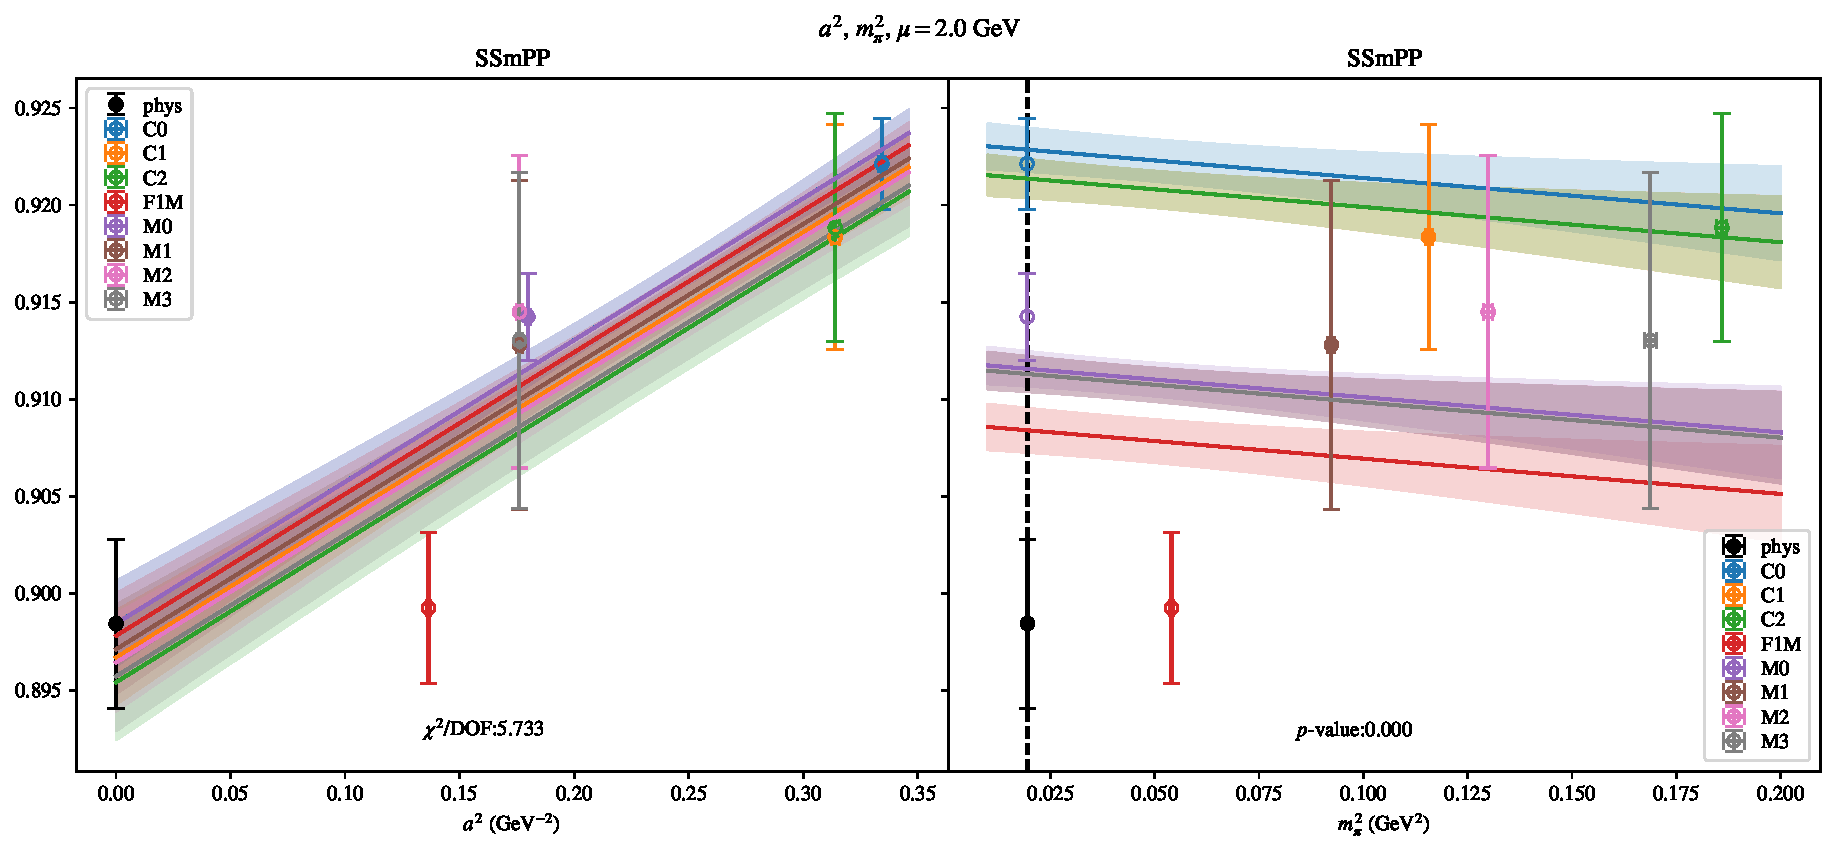
\includepdf[link, pages=-]{SSmPP/NPR/bag_a2m2_20.pdf}
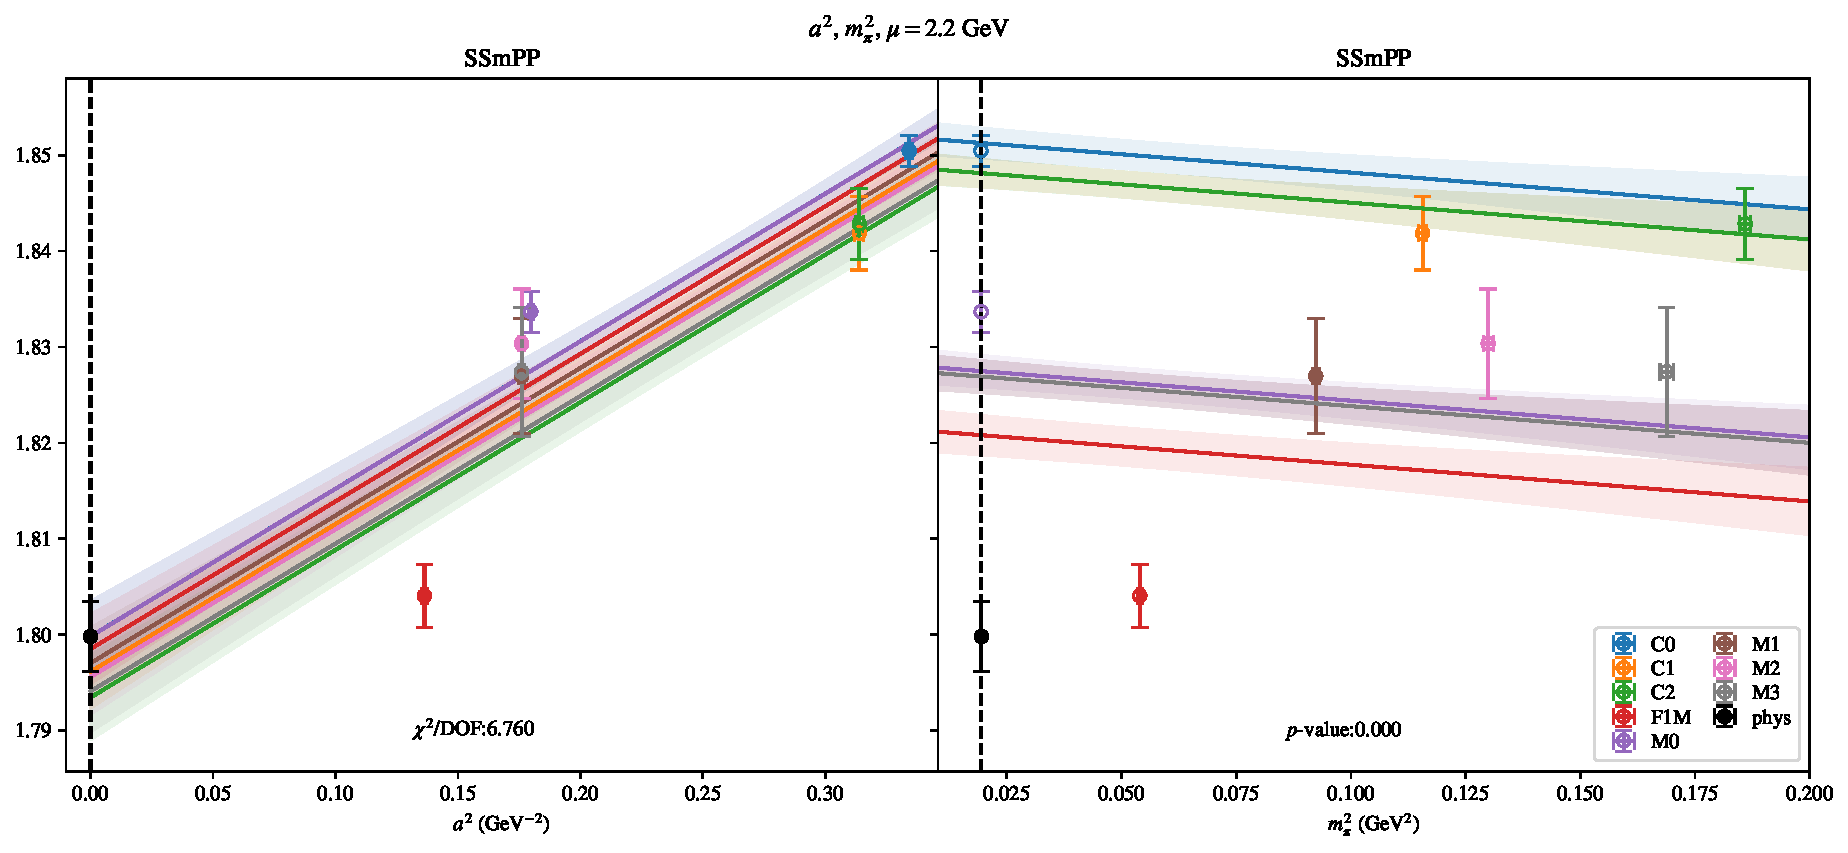
\includepdf[link, pages=-]{SSmPP/NPR/bag_a2m2_22.pdf}
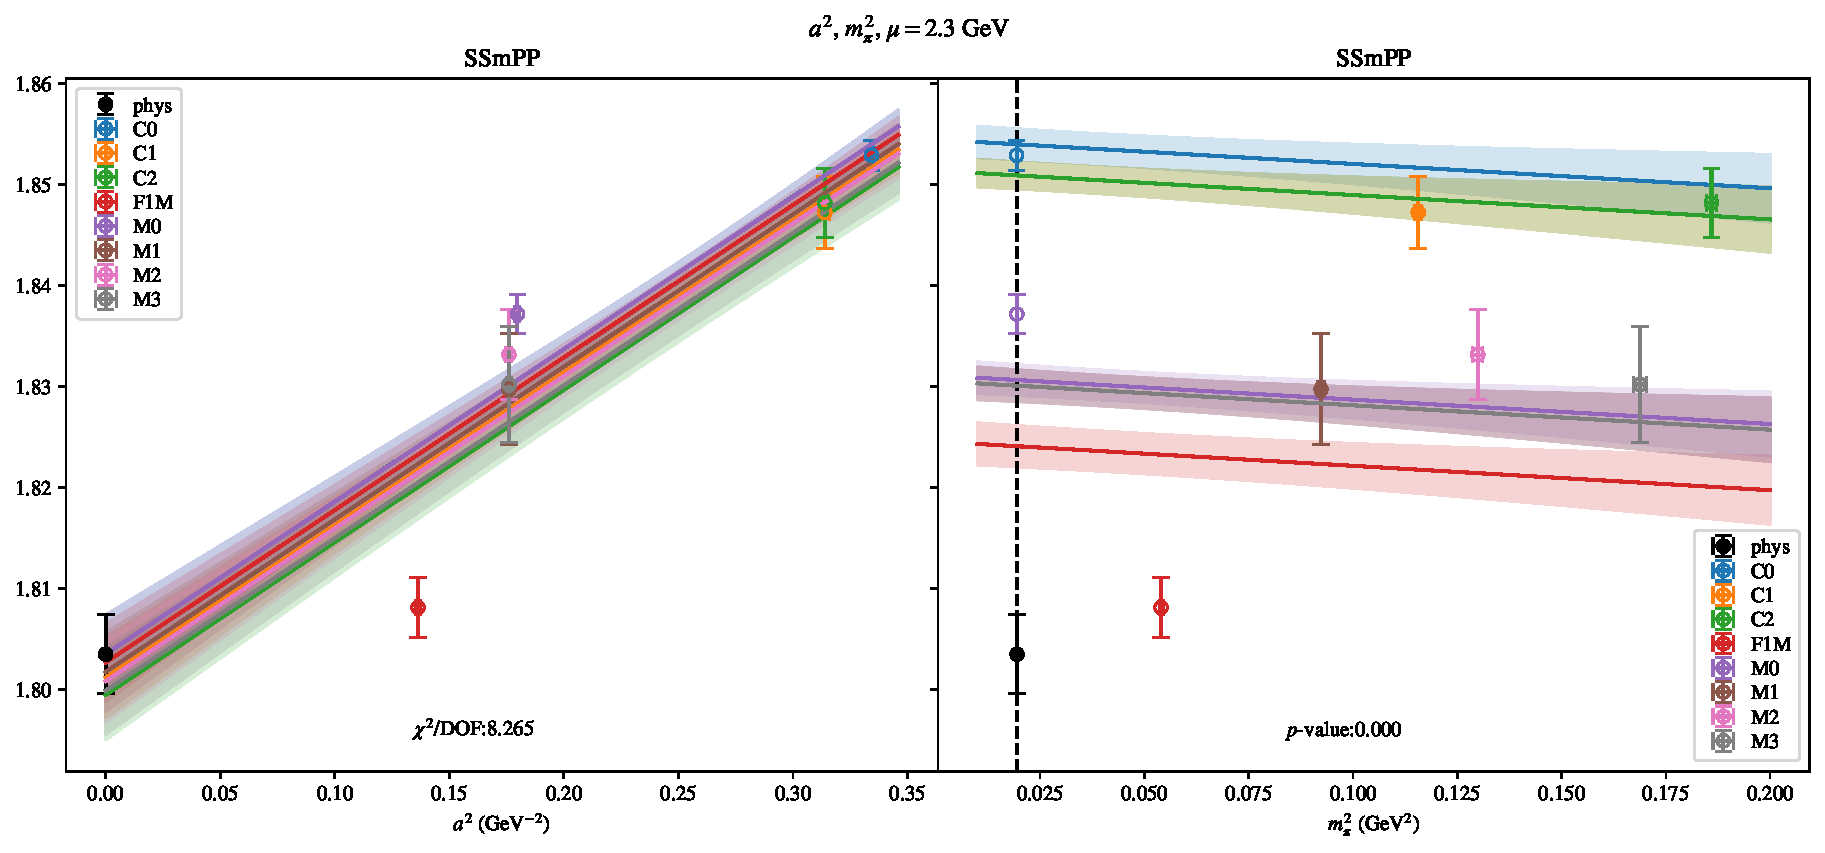
\includepdf[link, pages=-]{SSmPP/NPR/bag_a2m2_23.pdf}
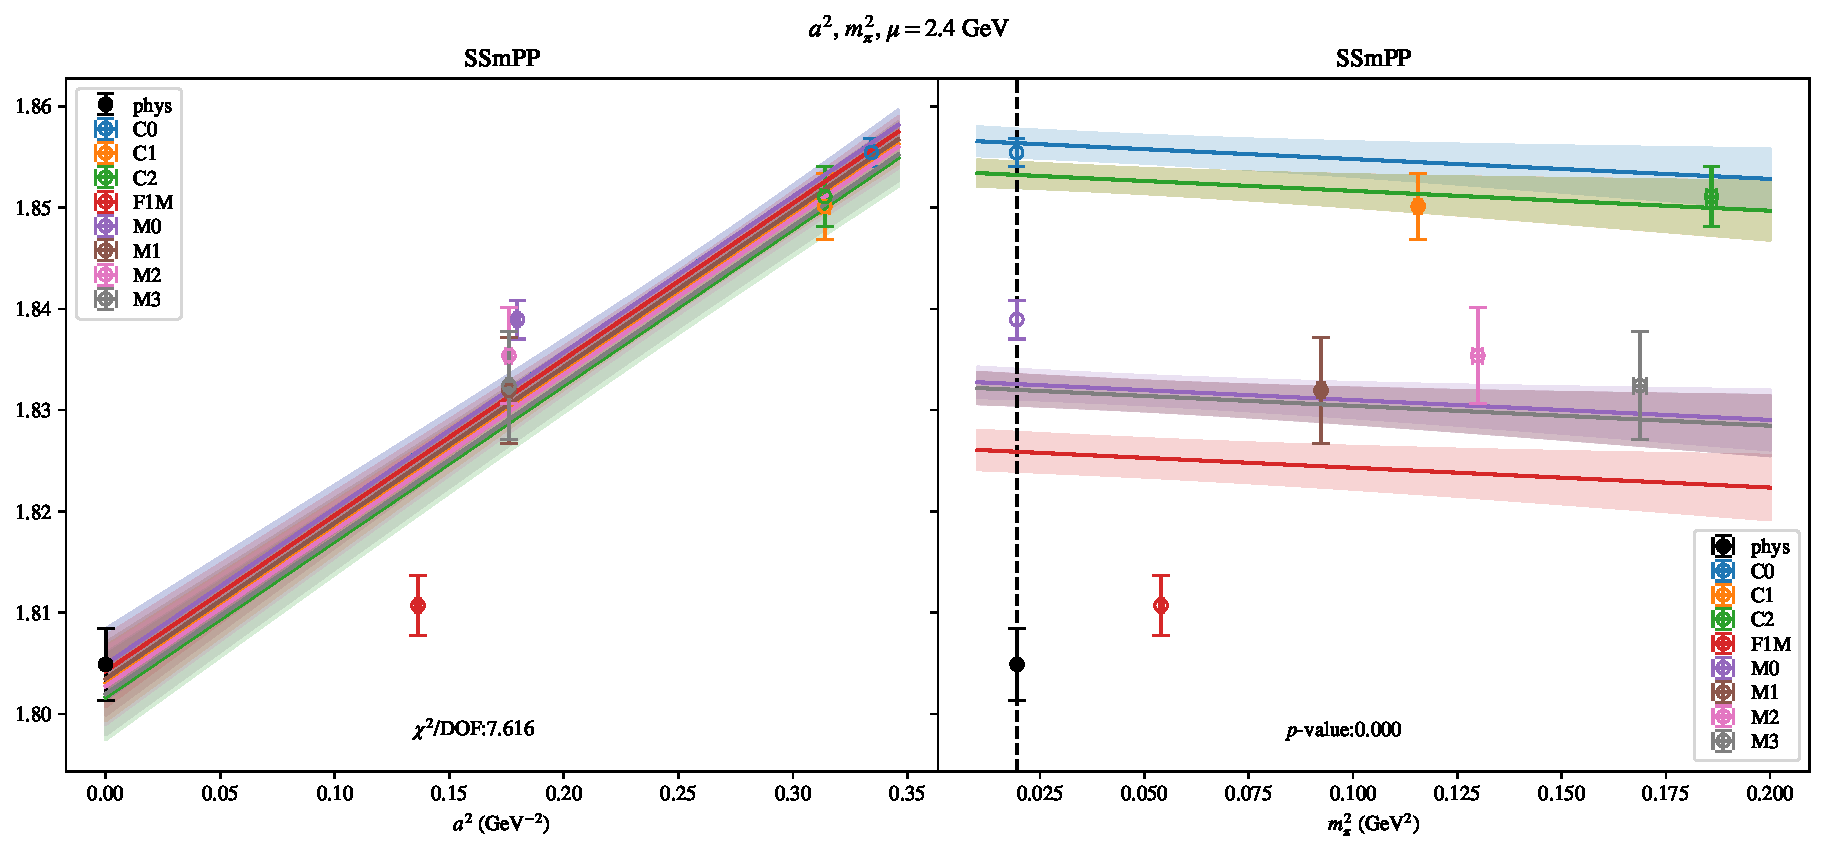
\includepdf[link, pages=-]{SSmPP/NPR/bag_a2m2_24.pdf}
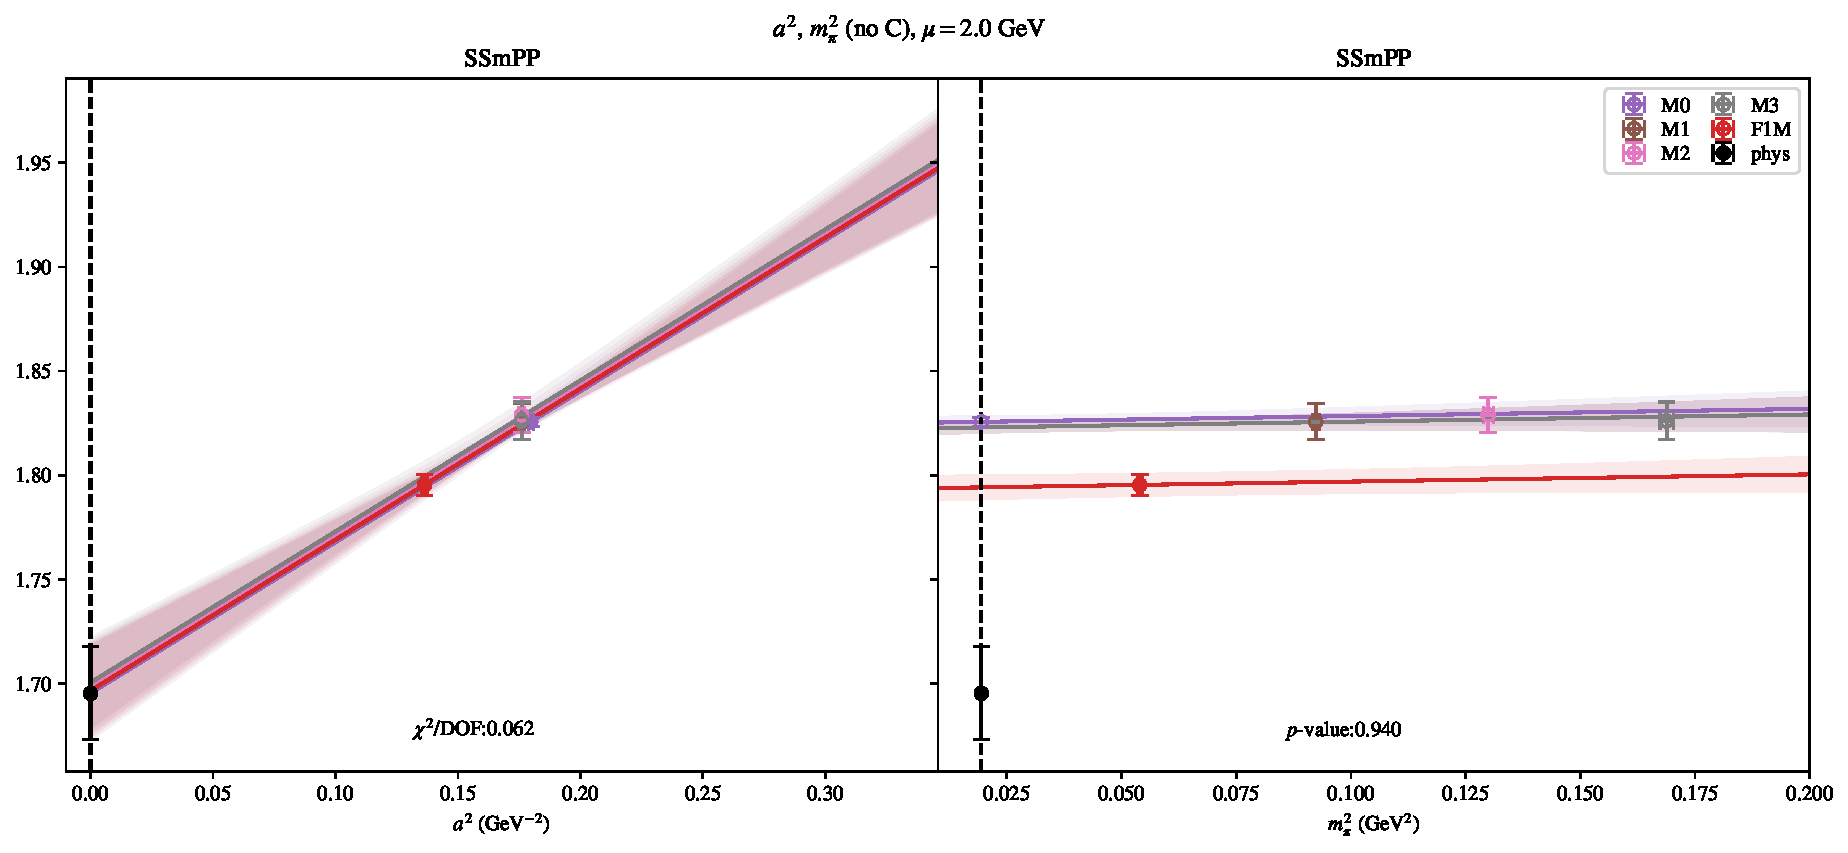
\includepdf[link, pages=-]{SSmPP/NPR/bag_a2m2noC_20.pdf}
\includepdf[link, pages=-]{SSmPP/NPR/bag_a2m2noC_22.pdf}
\includepdf[link, pages=-]{SSmPP/NPR/bag_a2m2noC_23.pdf}
\includepdf[link, pages=-]{SSmPP/NPR/bag_a2m2noC_24.pdf}
\includepdf[link, pages=-]{SSmPP/NPR/bag_a2a4m2_20.pdf}
\includepdf[link, pages=-]{SSmPP/NPR/bag_a2a4m2_22.pdf}
\includepdf[link, pages=-]{SSmPP/NPR/bag_a2a4m2_23.pdf}
\includepdf[link, pages=-]{SSmPP/NPR/bag_a2a4m2_24.pdf}
\includepdf[link, pages=-]{SSmPP/NPR/bag_a2m2mcut_20.pdf}
\includepdf[link, pages=-]{SSmPP/NPR/bag_a2m2mcut_22.pdf}
\includepdf[link, pages=-]{SSmPP/NPR/bag_a2m2mcut_23.pdf}
\includepdf[link, pages=-]{SSmPP/NPR/bag_a2m2mcut_24.pdf}
\includepdf[link, pages=-]{SSmPP/NPR/bag_a2m2delm_20.pdf}
\includepdf[link, pages=-]{SSmPP/NPR/bag_a2m2delm_22.pdf}
\includepdf[link, pages=-]{SSmPP/NPR/bag_a2m2delm_23.pdf}
\includepdf[link, pages=-]{SSmPP/NPR/bag_a2m2delm_24.pdf}
\clearpage
\section{$\mathcal{B}_4$}
\begin{table}[h!]
\begin{center}
\begin{tabular}{|c|c|c|c|c|c|}
\hline
$\mu$ (GeV) & $a^2$, $m_\pi^2$& $a^2$, $m_\pi^2$ (no C)& $a^2$, $m_\pi^2$, $a^4$& $a^2$, $m_\pi^2$ (no M3, C2)& $a^2$, $m_\pi^2$, $\delta m_s$\\
\hline
2.0& \hyperlink{SSpPP/NPR/bag_a2m2_20.pdf.1}{\textbf{-0.9273(27)}: 1.062 (0.379)} & \hyperlink{SSpPP/NPR/bag_a2m2noC_20.pdf.1}{\textbf{-0.943(11)}: 0.692 (0.501)} & \hyperlink{SSpPP/NPR/bag_a2a4m2_20.pdf.1}{\textbf{-0.951(19)}: 0.792 (0.53)} & \hyperlink{SSpPP/NPR/bag_a2m2mcut_20.pdf.1}{\textbf{-0.9266(28)}: 0.776 (0.507)} & \hyperlink{SSpPP/NPR/bag_a2m2delm_20.pdf.1}{\textbf{-0.9274(28)}: 1.23 (0.296)}\\
2.2& \hyperlink{SSpPP/NPR/bag_a2m2_22.pdf.1}{\textbf{-0.9080(22)}: 2.178 (0.054)} & \hyperlink{SSpPP/NPR/bag_a2m2noC_22.pdf.1}{\textbf{-0.9283(91)}: 0.738 (0.478)} & \hyperlink{SSpPP/NPR/bag_a2a4m2_22.pdf.1}{\textbf{-0.933(15)}: 1.886 (0.11)} & \hyperlink{SSpPP/NPR/bag_a2m2mcut_22.pdf.1}{\textbf{-0.9072(23)}: 1.997 (0.112)} & \hyperlink{SSpPP/NPR/bag_a2m2delm_22.pdf.1}{\textbf{-0.9080(22)}: 2.52 (0.039)}\\
2.3& \hyperlink{SSpPP/NPR/bag_a2m2_23.pdf.1}{\textbf{-0.8987(22)}: 3.165 (0.007)} & \hyperlink{SSpPP/NPR/bag_a2m2noC_23.pdf.1}{\textbf{-0.9210(89)}: 1.069 (0.343)} & \hyperlink{SSpPP/NPR/bag_a2a4m2_23.pdf.1}{\textbf{-0.924(14)}: 2.981 (0.018)} & \hyperlink{SSpPP/NPR/bag_a2m2mcut_23.pdf.1}{\textbf{-0.8983(23)}: 3.227 (0.021)} & \hyperlink{SSpPP/NPR/bag_a2m2delm_23.pdf.1}{\textbf{-0.8988(21)}: 3.92 (0.003)}\\
2.4& \hyperlink{SSpPP/NPR/bag_a2m2_24.pdf.1}{\textbf{-0.8909(22)}: 3.776 (0.002)} & \hyperlink{SSpPP/NPR/bag_a2m2noC_24.pdf.1}{\textbf{-0.9139(85)}: 1.269 (0.281)} & \hyperlink{SSpPP/NPR/bag_a2a4m2_24.pdf.1}{\textbf{-0.917(14)}: 3.72 (0.005)} & \hyperlink{SSpPP/NPR/bag_a2m2mcut_24.pdf.1}{\textbf{-0.8905(23)}: 4.145 (0.006)} & \hyperlink{SSpPP/NPR/bag_a2m2delm_24.pdf.1}{\textbf{-0.8909(21)}: 4.76 (0.001)}\\
\hline
\end{tabular}
\caption{Physical point value from chiral and continuum extrapolation at renormalisation scale $\mu$. Entries are \textbf{value(error)}: $\chi^2/\text{DOF}$ ($p$-value).}
\end{center}
\end{table}
\begin{table}[h!]
\begin{center}
\begin{tabular}{|c c|c|c|c|c|c|}
\hline
$\mu$ (GeV) &  & $a^2$, $m_\pi^2$& $a^2$, $m_\pi^2$ (no C)& $a^2$, $m_\pi^2$, $a^4$& $a^2$, $m_\pi^2$ (no M3, C2)& $a^2$, $m_\pi^2$, $\delta m_s$\\
\hline
\multirow{3}{0.5in}{2.0} & $\alpha$ & -0.349(11)& -0.257(67)& -0.13(17)& -0.351(11)& -0.350(11)\\
 & $\beta$ & -0.00700(28)& -0.00694(49)& -0.00705(29)& -0.00767(47)& -0.00721(52)\\
 & $\gamma$ &  &  & -0.44(34)&  & 0.009(19)\\
\hline
\multirow{3}{0.5in}{2.2} & $\alpha$ & -0.3788(86)& -0.260(52)& -0.15(14)& -0.3807(90)& -0.3794(85)\\
 & $\beta$ & -0.00678(19)& -0.00643(39)& -0.00686(19)& -0.00733(32)& -0.00701(40)\\
 & $\gamma$ &  &  & -0.46(28)&  & 0.009(15)\\
\hline
\multirow{3}{0.5in}{2.3} & $\alpha$ & -0.3959(87)& -0.267(51)& -0.16(13)& -0.3965(92)& -0.3964(83)\\
 & $\beta$ & -0.00687(18)& -0.00642(33)& -0.00696(19)& -0.00739(30)& -0.00706(37)\\
 & $\gamma$ &  &  & -0.47(26)&  & 0.008(13)\\
\hline
\multirow{3}{0.5in}{2.4} & $\alpha$ & -0.4106(87)& -0.277(49)& -0.17(13)& -0.4107(93)& -0.4111(84)\\
 & $\beta$ & -0.00683(17)& -0.00636(29)& -0.00692(17)& -0.00732(28)& -0.00702(35)\\
 & $\gamma$ &  &  & -0.48(26)&  & 0.008(13)\\
\hline
\end{tabular}
\caption{Fit values of coefficients in $Q = Q_{phys} + \mathbf{\alpha} a^2 + \mathbf{\beta}\left(\frac{m_\pi^2}{f_\pi^2}-\frac{m_{\pi,PDG}^2}{f_\pi^2}\right) + \gamma(\ldots)$}
\end{center}
\end{table}
\includepdf[link, pages=-]{SSpPP/NPR/bag_a2m2_20.pdf}
\includepdf[link, pages=-]{SSpPP/NPR/bag_a2m2_22.pdf}
\includepdf[link, pages=-]{SSpPP/NPR/bag_a2m2_23.pdf}
\includepdf[link, pages=-]{SSpPP/NPR/bag_a2m2_24.pdf}
\includepdf[link, pages=-]{SSpPP/NPR/bag_a2m2noC_20.pdf}
\includepdf[link, pages=-]{SSpPP/NPR/bag_a2m2noC_22.pdf}
\includepdf[link, pages=-]{SSpPP/NPR/bag_a2m2noC_23.pdf}
\includepdf[link, pages=-]{SSpPP/NPR/bag_a2m2noC_24.pdf}
\includepdf[link, pages=-]{SSpPP/NPR/bag_a2a4m2_20.pdf}
\includepdf[link, pages=-]{SSpPP/NPR/bag_a2a4m2_22.pdf}
\includepdf[link, pages=-]{SSpPP/NPR/bag_a2a4m2_23.pdf}
\includepdf[link, pages=-]{SSpPP/NPR/bag_a2a4m2_24.pdf}
\includepdf[link, pages=-]{SSpPP/NPR/bag_a2m2mcut_20.pdf}
\includepdf[link, pages=-]{SSpPP/NPR/bag_a2m2mcut_22.pdf}
\includepdf[link, pages=-]{SSpPP/NPR/bag_a2m2mcut_23.pdf}
\includepdf[link, pages=-]{SSpPP/NPR/bag_a2m2mcut_24.pdf}
\includepdf[link, pages=-]{SSpPP/NPR/bag_a2m2delm_20.pdf}
\includepdf[link, pages=-]{SSpPP/NPR/bag_a2m2delm_22.pdf}
\includepdf[link, pages=-]{SSpPP/NPR/bag_a2m2delm_23.pdf}
\includepdf[link, pages=-]{SSpPP/NPR/bag_a2m2delm_24.pdf}
\clearpage
\section{$\mathcal{B}_5$}
\begin{table}[h!]
\begin{center}
\begin{tabular}{|c|c|c|c|c|c|}
\hline
$\mu$ (GeV) & $a^2$, $m_\pi^2$& $a^2$, $m_\pi^2$ (no C)& $a^2$, $m_\pi^2$, $a^4$& $a^2$, $m_\pi^2$ (no M3, C2)& $a^2$, $m_\pi^2$, $\delta m_s$\\
\hline
2.0& \hyperlink{TT/NPR/bag_a2m2_20.pdf.1}{\textbf{-0.3620(63)}: 0.027 (1.0)} & \hyperlink{TT/NPR/bag_a2m2noC_20.pdf.1}{\textbf{-0.371(28)}: 0.004 (0.996)} & \hyperlink{TT/NPR/bag_a2a4m2_20.pdf.1}{\textbf{-0.377(45)}: 0.007 (1.0)} & \hyperlink{TT/NPR/bag_a2m2mcut_20.pdf.1}{\textbf{-0.3618(67)}: 0.038 (0.99)} & \hyperlink{TT/NPR/bag_a2m2delm_20.pdf.1}{\textbf{-0.3619(64)}: 0.02 (0.999)}\\
2.2& \hyperlink{TT/NPR/bag_a2m2_22.pdf.1}{\textbf{-0.3594(52)}: 0.044 (0.999)} & \hyperlink{TT/NPR/bag_a2m2noC_22.pdf.1}{\textbf{-0.369(24)}: 0.003 (0.997)} & \hyperlink{TT/NPR/bag_a2a4m2_22.pdf.1}{\textbf{-0.374(37)}: 0.017 (0.999)} & \hyperlink{TT/NPR/bag_a2m2mcut_22.pdf.1}{\textbf{-0.3595(59)}: 0.059 (0.981)} & \hyperlink{TT/NPR/bag_a2m2delm_22.pdf.1}{\textbf{-0.3594(55)}: 0.032 (0.998)}\\
2.3& \hyperlink{TT/NPR/bag_a2m2_23.pdf.1}{\textbf{-0.3583(48)}: 0.05 (0.999)} & \hyperlink{TT/NPR/bag_a2m2noC_23.pdf.1}{\textbf{-0.367(21)}: 0.006 (0.994)} & \hyperlink{TT/NPR/bag_a2a4m2_23.pdf.1}{\textbf{-0.370(34)}: 0.03 (0.998)} & \hyperlink{TT/NPR/bag_a2m2mcut_23.pdf.1}{\textbf{-0.3582(48)}: 0.059 (0.981)} & \hyperlink{TT/NPR/bag_a2m2delm_23.pdf.1}{\textbf{-0.3583(48)}: 0.042 (0.997)}\\
2.4& \hyperlink{TT/NPR/bag_a2m2_24.pdf.1}{\textbf{-0.3574(44)}: 0.059 (0.998)} & \hyperlink{TT/NPR/bag_a2m2noC_24.pdf.1}{\textbf{-0.366(19)}: 0.01 (0.99)} & \hyperlink{TT/NPR/bag_a2a4m2_24.pdf.1}{\textbf{-0.369(31)}: 0.037 (0.997)} & \hyperlink{TT/NPR/bag_a2m2mcut_24.pdf.1}{\textbf{-0.3575(49)}: 0.074 (0.974)} & \hyperlink{TT/NPR/bag_a2m2delm_24.pdf.1}{\textbf{-0.3574(44)}: 0.058 (0.994)}\\
\hline
\end{tabular}
\caption{Physical point value from chiral and continuum extrapolation at renormalisation scale $\mu$. Entries are \textbf{value(error)}: $\chi^2/\text{DOF}$ ($p$-value).}
\end{center}
\end{table}
\begin{table}[h!]
\begin{center}
\begin{tabular}{|c c|c|c|c|c|c|}
\hline
$\mu$ (GeV) &  & $a^2$, $m_\pi^2$& $a^2$, $m_\pi^2$ (no C)& $a^2$, $m_\pi^2$, $a^4$& $a^2$, $m_\pi^2$ (no M3, C2)& $a^2$, $m_\pi^2$, $\delta m_s$\\
\hline
\multirow{3}{0.5in}{2.0} & $\alpha$ & 0.008(23)& 0.06(16)& 0.14(41)& 0.007(24)& 0.006(23)\\
 & $\beta$ & -0.00245(65)& -0.0024(11)& -0.00248(67)& -0.0026(11)& -0.0027(13)\\
 & $\gamma$ &  &  & -0.27(82)&  & 0.011(46)\\
\hline
\multirow{3}{0.5in}{2.2} & $\alpha$ & 0.025(18)& 0.08(13)& 0.15(34)& 0.025(21)& 0.024(20)\\
 & $\beta$ & -0.00232(54)& -0.00220(96)& -0.00237(54)& -0.00241(90)& -0.0026(10)\\
 & $\gamma$ &  &  & -0.26(68)&  & 0.011(37)\\
\hline
\multirow{3}{0.5in}{2.3} & $\alpha$ & 0.034(17)& 0.09(12)& 0.14(31)& 0.034(18)& 0.033(18)\\
 & $\beta$ & -0.00240(54)& -0.00226(86)& -0.00244(52)& -0.00254(85)& -0.00264(99)\\
 & $\gamma$ &  &  & -0.22(62)&  & 0.010(35)\\
\hline
\multirow{3}{0.5in}{2.4} & $\alpha$ & 0.042(16)& 0.09(11)& 0.15(28)& 0.043(17)& 0.042(16)\\
 & $\beta$ & -0.00240(46)& -0.00227(74)& -0.00244(45)& -0.00252(75)& -0.00261(84)\\
 & $\gamma$ &  &  & -0.22(57)&  & 0.008(29)\\
\hline
\end{tabular}
\caption{Fit values of coefficients in $Q = Q_{phys} + \mathbf{\alpha} a^2 + \mathbf{\beta}\left(\frac{m_\pi^2}{f_\pi^2}-\frac{m_{\pi,PDG}^2}{f_\pi^2}\right) + \gamma(\ldots)$}
\end{center}
\end{table}
\includepdf[link, pages=-]{TT/NPR/bag_a2m2_20.pdf}
\includepdf[link, pages=-]{TT/NPR/bag_a2m2_22.pdf}
\includepdf[link, pages=-]{TT/NPR/bag_a2m2_23.pdf}
\includepdf[link, pages=-]{TT/NPR/bag_a2m2_24.pdf}
\includepdf[link, pages=-]{TT/NPR/bag_a2m2noC_20.pdf}
\includepdf[link, pages=-]{TT/NPR/bag_a2m2noC_22.pdf}
\includepdf[link, pages=-]{TT/NPR/bag_a2m2noC_23.pdf}
\includepdf[link, pages=-]{TT/NPR/bag_a2m2noC_24.pdf}
\includepdf[link, pages=-]{TT/NPR/bag_a2a4m2_20.pdf}
\includepdf[link, pages=-]{TT/NPR/bag_a2a4m2_22.pdf}
\includepdf[link, pages=-]{TT/NPR/bag_a2a4m2_23.pdf}
\includepdf[link, pages=-]{TT/NPR/bag_a2a4m2_24.pdf}
\includepdf[link, pages=-]{TT/NPR/bag_a2m2mcut_20.pdf}
\includepdf[link, pages=-]{TT/NPR/bag_a2m2mcut_22.pdf}
\includepdf[link, pages=-]{TT/NPR/bag_a2m2mcut_23.pdf}
\includepdf[link, pages=-]{TT/NPR/bag_a2m2mcut_24.pdf}
\includepdf[link, pages=-]{TT/NPR/bag_a2m2delm_20.pdf}
\includepdf[link, pages=-]{TT/NPR/bag_a2m2delm_22.pdf}
\includepdf[link, pages=-]{TT/NPR/bag_a2m2delm_23.pdf}
\includepdf[link, pages=-]{TT/NPR/bag_a2m2delm_24.pdf}
\clearpage
\end{document}